\documentclass[12pt,a4paper]{report}
\usepackage[T5]{fontenc}
\usepackage[utf8]{inputenc}
\usepackage[vietnamese]{babel}
\usepackage[top=3cm,bottom=2cm,left=3cm,right=2cm,headheight=28pt]{geometry}
\usepackage{mathptmx}
\usepackage{setspace}
\onehalfspacing
\usepackage{graphicx}
\usepackage{array,longtable,booktabs}
\usepackage[table]{xcolor}
\usepackage{caption}
\captionsetup{font=small,labelfont=bf}
\usepackage{float}
\usepackage{fancyhdr}
\usepackage{lastpage}
\usepackage{enumitem}
\usepackage[hidelinks]{hyperref}

\setcounter{tocdepth}{2}
\setlength{\parindent}{1cm}
\setlength{\tabcolsep}{5pt}
\renewcommand{\arraystretch}{1.15}

% Cho phép ngắt trang linh hoạt, lấp đầy văn bản khi có trang hình [p]
\raggedbottom
\widowpenalty=1000
\clubpenalty=1000
\renewcommand{\floatpagefraction}{0.8}

\pagestyle{fancy}
\fancyhead{}
\fancyhead[L]{%
 \begin{tabular}{rl}
    \begin{picture}(25,15)(0,0)
    \put(0,-8){
\includegraphics[width=8mm,height=8mm]{logoITSGUsmall.png}}
   \end{picture}&
   \begin{tabular}{l}
      \textbf{\ttfamily Trường Đại học Sài Gòn}\\
      \textbf{\ttfamily Khoa Công Nghệ Thông Tin}
   \end{tabular}
 \end{tabular}
}
\fancyhead[R]{}
\fancyfoot{}
\fancyfoot[L]{\scriptsize \ttfamily Báo cáo đồ án môn Công nghệ Phần mềm -- BrewLite}
\fancyfoot[R]{\scriptsize \ttfamily Trang \thepage/\pageref{LastPage}}
\renewcommand{\headrulewidth}{0.3pt}
\renewcommand{\footrulewidth}{0.3pt}

\begin{document}

\begin{titlepage}
\thispagestyle{empty}
\begin{center}
TRƯỜNG ĐẠI HỌC SÀI GÒN \\
KHOA CÔNG NGHỆ THÔNG TIN
\end{center}
\vspace{1cm}
\begin{figure}[h!]
\begin{center}

\includegraphics[width=3.5cm]{logoITSGU.png}
\end{center}
\end{figure}
\vspace{1cm}
\begin{center}
{\Large\bfseries ĐỒ ÁN} \\
{\Large\bfseries CÔNG NGHỆ PHẦN MỀM}
\vspace{1cm}

{\large\bfseries ĐỀ TÀI: XÂY DỰNG PHẦN MỀM} \\
\vspace{0.5cm}
{\Large\bfseries Hệ thống đặt cà phê và thanh toán không dùng tiền mặt -- BrewLite} \\
\vspace{0.3cm}
(BrewLite Coffee Ordering System)
\end{center}
\vspace{2.5cm}
\begin{center}
\begin{tabular}{rl}
Giảng viên hướng dẫn: & Từ Lãng Phiêu \\
Nhóm: & 8 \\
\end{tabular}
\vspace{1cm}

Sinh viên thực hiện: \\
\vspace{0.3cm}
\begin{tabular}{|p{3.2cm}|p{6.8cm}|}
\hline
\centering\textbf{MSSV} & \textbf{Họ tên} \\
\hline
 & Võ Đức Hoàng Vinh \\ \hline
 & Hồ Hoàng Anh \\ \hline
 & Dương Thành Phát \\ \hline
 & Quách Thanh Phú \\ \hline
 & Đặng Lương Thế Anh \\ \hline
 & Nguyễn Hoàng Anh \\ \hline
 & Hoàng Trần Gia Phước \\ \hline
\end{tabular}
\end{center}
\vfill
\begin{center}
{\footnotesize Thành phố Hồ Chí Minh, tháng 11/2026}
\end{center}
\end{titlepage}

\chapter*{NHẬN XÉT CỦA GIẢNG VIÊN}
\addcontentsline{toc}{chapter}{Nhận xét của giảng viên}
\vspace{1cm}
\noindent\dotfill\\[1.2cm]
\noindent\dotfill\\[1.2cm]
\noindent\dotfill\\[1.2cm]
\noindent\dotfill\\[1.2cm]
\noindent\dotfill\\[1.2cm]
\noindent\dotfill\\[1.2cm]
\noindent\dotfill\\[1.2cm]
\noindent\dotfill\\[1.2cm]
\noindent\dotfill\\[1.2cm]
\noindent\dotfill
\newpage

\chapter*{LỜI MỞ ĐẦU}
\addcontentsline{toc}{chapter}{Lời mở đầu}

Trong những năm gần đây, thói quen tiêu dùng tại các cửa hàng đồ uống đã thay đổi rõ rệt: khách hàng ưu tiên sự nhanh chóng, tiện lợi và các phương thức thanh toán không dùng tiền mặt, trong khi các cửa hàng lại phải đối mặt với áp lực phục vụ ngày càng lớn vào giờ cao điểm. Việc tiếp nhận đơn hàng, pha chế và thu ngân theo phương thức thủ công bộc lộ nhiều hạn chế như xếp hàng chờ đợi lâu, sai sót trong ghi nhận yêu cầu của khách và khó kiểm soát nguyên liệu tồn kho, ảnh hưởng trực tiếp đến chất lượng dịch vụ và hiệu quả kinh doanh.

Xuất phát từ thực trạng đó, đề tài ``Hệ thống đặt cà phê và thanh toán không dùng tiền mặt -- BrewLite (BrewLite Coffee Ordering System)'' được thực hiện nhằm xây dựng một giải pháp phần mềm hỗ trợ số hóa toàn bộ quy trình đặt món -- thanh toán -- pha chế -- nhận món tại cửa hàng cà phê. Hệ thống cho phép khách hàng đặt đồ uống trực tuyến, tùy chọn kích cỡ và thành phần đi kèm, thanh toán an toàn qua cổng thanh toán điện tử, đồng thời giúp nhân viên quầy quản lý đơn hàng, thực đơn, tồn kho và doanh thu một cách tập trung, chính xác.

Báo cáo này trình bày quá trình phân tích, thiết kế và xây dựng hệ thống BrewLite theo đúng quy trình phát triển phần mềm. Chương 1 tập trung khai thác và phân tích yêu cầu, làm rõ bối cảnh dự án, các bên liên quan, nhu cầu và vấn đề hiện tại, từ đó xác định các yêu cầu chức năng và yêu cầu phi chức năng làm cơ sở cho các chương mô hình hóa, thiết kế kiến trúc và thiết kế chi tiết tiếp theo.

\tableofcontents
\newpage

\chapter{KHAI THÁC VÀ PHÂN TÍCH YÊU CẦU}

\section{Bối cảnh và các bên liên quan}

\subsection{Bối cảnh và phạm vi dự án}

Hiện nay, mô hình kinh doanh cà phê tại các đô thị đang phát triển nhanh chóng cả về số lượng cửa hàng lẫn nhu cầu tiêu dùng. Tuy nhiên, quy trình phục vụ tại phần lớn các cửa hàng vừa và nhỏ vẫn được tổ chức theo phương thức truyền thống: khách hàng đến trực tiếp quầy, xếp hàng chờ gọi món, nhân viên ghi nhận yêu cầu bằng lời nói hoặc trên giấy, sau đó thực hiện pha chế và thu tiền mặt tại quầy. Vào các khung giờ cao điểm như đầu giờ sáng hoặc giờ nghỉ trưa, lượng khách tập trung đông khiến hàng chờ kéo dài, thời gian phục vụ tăng lên đáng kể và trải nghiệm của khách hàng bị ảnh hưởng nghiêm trọng. Bên cạnh đó, việc truyền đạt yêu cầu hoàn toàn bằng lời nói rất dễ phát sinh sai sót, chẳng hạn như nhầm kích cỡ (size), mức đường, mức đá hoặc thành phần đi kèm (topping), dẫn đến việc phải pha chế lại, gây lãng phí nguyên liệu và làm chậm toàn bộ hàng đợi phía sau.

Một vấn đề khác không kém phần nghiêm trọng là công tác quản lý đơn hàng và tồn kho còn mang tính thủ công, thiếu đồng bộ. Đơn hàng được ghi chép rời rạc, khó tổng hợp doanh thu và khó truy vết khi xảy ra sai lệch; lượng nguyên liệu tồn kho (cà phê, sữa, đường, topping\dots{}) không được cập nhật theo thời gian thực, nên cửa hàng vẫn tiếp tục nhận đơn đối với những món đã hết nguyên liệu, hoặc ngược lại, phải hủy đơn và hoàn tiền cho khách sau khi đã thanh toán. Tình trạng ``bán âm'' tồn kho này không chỉ gây thiệt hại về kinh tế mà còn làm giảm uy tín của cửa hàng. Đồng thời, các chương trình ưu đãi và tích điểm cho khách hàng thân thiết, nếu có, cũng được thực hiện thủ công nên thiếu nhất quán, khó kiểm soát và dễ gian lận.

Xuất phát từ những hạn chế nêu trên, hệ thống BrewLite được đề xuất và xây dựng nhằm số hóa toàn bộ quy trình đặt món và thanh toán tại cửa hàng cà phê. BrewLite cho phép khách hàng chủ động đặt đồ uống ngay trên thiết bị cá nhân, tùy chọn size, topping, mức đường, mức đá và ghi chú riêng, sau đó thanh toán không dùng tiền mặt thông qua cổng thanh toán điện tử trước khi đến quầy nhận món. Về phía cửa hàng, hệ thống quản lý tập trung thực đơn, đơn hàng, nguyên liệu tồn kho, khuyến mãi và điểm thưởng trên một nền tảng duy nhất, với các cơ chế kỹ thuật chặt chẽ như máy trạng thái đơn hàng (PENDING $\rightarrow$ PAID $\rightarrow$ PREPARING $\rightarrow$ READY $\rightarrow$ COMPLETED), thanh toán chống trùng lặp (Idempotency) và khóa lạc quan (Optimistic Locking) chống bán âm tồn kho. Phạm vi của dự án bao gồm các nghiệp vụ đặt món, giỏ hàng, thanh toán trực tuyến, quản lý đơn hàng tại quầy, quản lý thực đơn và nguyên liệu, khuyến mãi, tích điểm và thống kê báo cáo cho một cửa hàng hoặc chuỗi cửa hàng cà phê quy mô vừa; hệ thống chưa bao gồm nghiệp vụ giao hàng tận nơi bởi đối tác vận chuyển bên thứ ba và quản lý nhân sự -- chấm công. Hệ thống được phát triển trên nền tảng web với Next.js ở phía giao diện người dùng (Frontend), NestJS ở phía xử lý nghiệp vụ (Backend) và hệ quản trị cơ sở dữ liệu PostgreSQL.

\subsection{Các bên liên quan chính}

Qua quá trình khảo sát thực tế tại các cửa hàng cà phê và đối chiếu theo yêu cầu của Assignment 2, nhóm thực hiện xác định hệ thống BrewLite có sáu bên liên quan chính (ba bên tương tác trực tiếp với phần mềm và ba bên tham gia quản lý, phát triển, nghiệm thu):

\begin{itemize}[leftmargin=*]
\item \textbf{Khách hàng (Customer):}
  \begin{itemize}[nosep]
  \item Là người sử dụng trực tiếp hệ thống để xem thực đơn, lựa chọn đồ uống và thực hiện đặt hàng.
  \item Thực hiện tùy chọn size, topping, mức đường, mức đá, quản lý giỏ hàng và thanh toán không dùng tiền mặt.
  \item Theo dõi trạng thái đơn hàng theo thời gian thực, nhận món tại quầy, xem lịch sử mua hàng, đánh giá món và sử dụng điểm thưởng, mã khuyến mãi.
  \end{itemize}

\item \textbf{Nhân viên quầy (Barista):}
  \begin{itemize}[nosep]
  \item Là người tiếp nhận các đơn hàng đã được thanh toán thành công trên bảng Kanban tại khu vực pha chế.
  \item Xem công thức định lượng chi tiết, thực hiện pha chế và cập nhật trạng thái đơn hàng theo quy trình (đang pha chế, đã sẵn sàng, đã hoàn thành).
  \item Phản hồi kịp thời cho quản lý cửa hàng khi nguyên liệu sắp hết, hết hàng hoặc phát sinh sự cố đối với đơn hàng.
  \end{itemize}

\item \textbf{Quản lý cửa hàng / Quản trị viên (Admin / Product Owner):}
  \begin{itemize}[nosep]
  \item Quản trị thực đơn, biến thể sản phẩm, công thức định lượng, kho nguyên liệu và lập phiếu nhập kho từ nhà cung cấp.
  \item Theo dõi thống kê doanh thu, quản lý mã khuyến mãi, kiểm duyệt đánh giá và quản lý tài khoản nhân sự/khách hàng.
  \end{itemize}

\item \textbf{Đơn vị thanh toán (Payment Gateway):}
  \begin{itemize}[nosep]
  \item Là hệ thống bên ngoài (mô phỏng qua Mock Gateway và ứng dụng MBBank VietQR Simulator) cung cấp dịch vụ thanh toán không dùng tiền mặt.
  \item Tiếp nhận yêu cầu thanh toán từ BrewLite, xử lý giao dịch và gửi kết quả đồng bộ về hệ thống.
  \end{itemize}

\item \textbf{Nhóm phát triển (Development Team):}
  \begin{itemize}[nosep]
  \item Nhóm 7 thành viên chịu trách nhiệm khai thác yêu cầu, mô hình hóa UML, thiết kế kiến trúc, lập trình Frontend/Backend, kiểm thử tự động và triển khai CI/CD.
  \end{itemize}

\item \textbf{Giảng viên hướng dẫn / Khách hàng nghiệm thu:}
  \begin{itemize}[nosep]
  \item Đánh giá quy trình phát triển tuần tự qua các Sprint, chất lượng tạo phẩm tài liệu, mã nguồn, kiểm thử và sản phẩm triển khai thực tế.
  \end{itemize}
\end{itemize}

\subsection{Nhu cầu hiện tại và vấn đề của từng bên}

Kết quả khảo sát cho thấy mỗi bên liên quan đều có những nhu cầu nghiệp vụ đặc thù, đồng thời đang gặp phải những vấn đề riêng trong quy trình vận hành hiện tại. Nội dung phân tích chi tiết được tổng hợp trong Bảng 1.1.

\begin{longtable}{>{\raggedright\arraybackslash}p{3.0cm}>{\raggedright\arraybackslash}p{6.0cm}>{\raggedright\arraybackslash}p{6.0cm}}
\caption{Nhu cầu hiện tại và vấn đề của từng bên liên quan}\\
\hline
\rowcolor{gray!20} \textbf{Bên liên quan} & \textbf{Nhu cầu hiện tại} & \textbf{Vấn đề hiện tại} \\
\hline
\endfirsthead
\hline
\rowcolor{gray!20} \textbf{Bên liên quan} & \textbf{Nhu cầu hiện tại} & \textbf{Vấn đề hiện tại} \\
\hline
\endhead
Khách hàng (Customer) 
& -- Đặt món nhanh chóng, không phải xếp hàng chờ đợi lâu tại quầy, đặc biệt vào giờ cao điểm. \newline
-- Tùy chọn linh hoạt size, topping, mức đường, mức đá theo sở thích cá nhân. \newline
-- Thanh toán tiện lợi, an toàn bằng phương thức không dùng tiền mặt. \newline
-- Biết chính xác trạng thái đơn hàng và thời điểm đến nhận món; được tích điểm và hưởng ưu đãi khi mua hàng thường xuyên. 
& -- Phải xếp hàng và chờ đợi lâu; thời gian chờ tăng mạnh vào giờ cao điểm. \newline
-- Yêu cầu gọi món bằng lời nói dễ bị ghi nhận sai (nhầm size, topping, mức đường/đá), phải chờ pha chế lại. \newline
-- Thanh toán tiền mặt gây bất tiện, mất thời gian thối tiền và tiềm ẩn rủi ro về vệ sinh, an toàn. \newline
-- Không biết đơn của mình đang ở trạng thái nào, phải chủ động hỏi nhân viên; điểm thưởng (nếu có) được ghi nhận thủ công, thiếu minh bạch. \\
\hline
Nhân viên quầy (Barista) 
& -- Tiếp nhận danh sách đơn hàng rõ ràng, có thứ tự ưu tiên, kèm đầy đủ chi tiết về size, topping và ghi chú của khách. \newline
-- Có công cụ cập nhật trạng thái đơn hàng nhanh chóng để khách hàng chủ động theo dõi. \newline
-- Được cảnh báo sớm khi nguyên liệu sắp hết để tránh nhận đơn đối với món không còn khả năng phục vụ. 
& -- Đơn hàng được ghi bằng giấy hoặc truyền miệng nên dễ nhầm lẫn, khó đọc, dễ thất lạc khi lượng đơn tăng cao. \newline
-- Không có hàng đợi đơn hàng tập trung; việc sắp xếp thứ tự pha chế phụ thuộc vào trí nhớ, dễ gây bỏ sót hoặc làm sai thứ tự. \newline
-- Chỉ phát hiện hết nguyên liệu khi đang pha chế, dẫn đến hủy đơn, hoàn tiền và làm khách hàng không hài lòng. \newline
-- Phải vừa pha chế vừa thu tiền và giải thích cho khách, gây quá tải trong giờ cao điểm. \\
\hline
\end{longtable}

\subsection{Lợi ích BrewLite mang lại cho từng bên}

Việc triển khai hệ thống BrewLite mang lại lợi ích thiết thực và có thể đo lường được cho từng bên liên quan, đồng thời khắc phục trực tiếp các vấn đề đã phân tích tại mục 1.1.3. Các lợi ích cụ thể được trình bày trong Bảng 1.2.

\begin{longtable}{>{\raggedright\arraybackslash}p{3.4cm}>{\raggedright\arraybackslash}p{11.8cm}}
\caption{Lợi ích BrewLite mang lại cho từng bên liên quan}\\
\hline
\rowcolor{gray!20} \textbf{Bên liên quan} & \textbf{Lợi ích đạt được khi triển khai hệ thống} \\
\hline
\endfirsthead
\hline
\rowcolor{gray!20} \textbf{Bên liên quan} & \textbf{Lợi ích đạt được khi triển khai hệ thống} \\
\hline
\endhead
Khách hàng (Customer) 
& -- Đặt món trước ngay trên điện thoại/máy tính và chỉ đến quầy nhận món khi đơn ở trạng thái READY, loại bỏ gần như hoàn toàn thời gian xếp hàng chờ gọi món. \newline
-- Tùy chọn size, topping, mức đường, mức đá và ghi chú được lưu chính xác trên đơn điện tử, hạn chế tối đa sai sót do truyền miệng. \newline
-- Thanh toán không dùng tiền mặt nhanh chóng, an toàn; cơ chế Idempotency đảm bảo mỗi đơn chỉ bị trừ tiền một lần duy nhất dù khách thao tác lại hoặc mạng chập chờn. \newline
-- Theo dõi trạng thái đơn hàng theo thời gian thực qua máy trạng thái chặt chẽ (PENDING $\rightarrow$ PAID $\rightarrow$ PREPARING $\rightarrow$ READY $\rightarrow$ COMPLETED); điểm thưởng được tự động cộng sau mỗi hóa đơn và có thể quy đổi ở các lần mua tiếp theo; được áp dụng mã khuyến mãi rõ ràng, minh bạch. \\
\hline
Nhân viên quầy (Barista) 
& -- Tiếp nhận đơn hàng trên một hàng đợi tập trung, sắp xếp theo thứ tự thanh toán, với đầy đủ chi tiết pha chế, giúp pha chế chính xác và đúng thứ tự. \newline
-- Chỉ cần thao tác cập nhật trạng thái đơn (PREPARING $\rightarrow$ READY $\rightarrow$ COMPLETED) trên hệ thống, không phải gọi tên, ghi giấy hay thu tiền mặt, giảm đáng kể áp lực trong giờ cao điểm. \newline
-- Nhận cảnh báo tồn kho kịp thời và chủ động tạm ngưng bán các món hết nguyên liệu, tránh tình trạng pha chế dở mới phát hiện thiếu nguyên liệu. \newline
-- Giảm tranh cãi và sai sót với khách hàng do mọi thông tin đơn hàng đều được lưu trữ và hiển thị thống nhất trên hệ thống. \\
\hline
Đơn vị thanh toán (Payment Gateway) 
& -- Nhận lưu lượng giao dịch ổn định, có cấu trúc từ hệ thống BrewLite với mã giao dịch và khóa Idempotency rõ ràng cho từng đơn hàng, giúp việc xử lý, truy vết và đối soát diễn ra chính xác. \newline
-- Giảm các giao dịch trùng lặp và tranh chấp hoàn tiền nhờ cơ chế xác thực kết quả thanh toán qua callback/webhook có kiểm tra chữ ký trước khi hệ thống ghi nhận đơn hàng. \\
\hline
\end{longtable}

\subsection{Phạm vi dự án, giả định và ràng buộc}

Phạm vi trong MVP (In-Scope), phần ngoài phạm vi (Out-of-Scope), giả định và các ràng buộc kỹ thuật bắt buộc của Assignment 2 được tổng hợp trong Bảng 1.3.

\begin{longtable}{>{\raggedright\arraybackslash}p{3.8cm}>{\raggedright\arraybackslash}p{11.4cm}}
\caption{Phạm vi, giả định và ràng buộc của dự án BrewLite}\\
\hline
\rowcolor{gray!20} \textbf{Hạng mục} & \textbf{Nội dung chi tiết} \\
\hline
\endfirsthead
\hline
\rowcolor{gray!20} \textbf{Hạng mục} & \textbf{Nội dung chi tiết} \\
\hline
\endhead
Trong phạm vi MVP (In-Scope) & -- Xem thực đơn số, tìm kiếm, lọc danh mục, xem chi tiết Size S/M/L, Topping, đường/đá và trạng thái còn/hết nguyên liệu. \newline
-- Giỏ hàng lưu cục bộ trên trình duyệt, tự động tính tổng tiền, áp dụng mã Voucher và sử dụng điểm thưởng. \newline
-- Đăng ký tài khoản Customer, đăng nhập JWT, làm mới phiên, xem thông tin cá nhân, đổi mật khẩu và đăng xuất. \newline
-- Tạo đơn hàng (PENDING), thanh toán không tiền mặt mô phỏng (Ví/Thẻ/MBBank VietQR) đảm bảo Idempotency, trừ kho bằng Optimistic Locking (OCC). \newline
-- Theo dõi trạng thái đơn, hủy đơn (PENDING/PAID) hoàn kho, xem lịch sử và đánh giá món đã mua. \newline
-- Bảng Kanban FIFO cho Barista (PAID $\rightarrow$ PREPARING $\rightarrow$ READY $\rightarrow$ COMPLETED) và xem công thức pha chế. \newline
-- Dashboard Admin: thống kê doanh thu, quản lý kho/nhập hàng, sản phẩm/công thức, khuyến mãi, kiểm duyệt đánh giá và nhân sự/khách hàng. \\
\hline
Ngoài phạm vi (Out-of-Scope) & -- Giao hàng tận nơi qua đối tác vận chuyển bên thứ ba (Grab, ShopeeFood). \newline
-- Kết nối cổng thanh toán tiền thật ngoài môi trường mô phỏng và phần cứng máy in hóa đơn nhiệt tại quầy. \newline
-- Quản lý chấm công, tính lương nhân sự. \\
\hline
Giả định (Assumptions) & -- Khách hàng và nhân viên sử dụng trình duyệt web hiện đại có kết nối Internet. \newline
-- Dịch vụ cổng thanh toán mô phỏng và ứng dụng MBBank Simulator hoạt động ổn định khi kiểm thử. \\
\hline
Ràng buộc kỹ thuật & -- Frontend sử dụng Next.js 14 theo hướng mobile-first/PWA; Backend sử dụng NestJS 10; CSDL là PostgreSQL 16 (Prisma ORM). \newline
-- Đóng gói triển khai qua Docker Compose và tự động kiểm tra chất lượng qua CI/CD. \\
\hline
\end{longtable}

\section{Yêu cầu hệ thống}

Trên cơ sở bối cảnh, nhu cầu và các vấn đề đã phân tích tại mục 1.1, nhóm thực hiện tiến hành xác định yêu cầu cho hệ thống BrewLite theo hai nhóm chính: yêu cầu chức năng (Functional Requirements) -- mô tả những dịch vụ mà hệ thống phải cung cấp, và yêu cầu phi chức năng (Non-functional Requirements) -- mô tả các ràng buộc về chất lượng, hiệu năng, bảo mật và khả năng triển khai mà hệ thống phải thỏa mãn trong quá trình vận hành.

\subsection{Yêu cầu chức năng}

Yêu cầu chức năng của hệ thống BrewLite được tổ chức theo các nhóm tác nhân chính là Nhân viên quầy (Barista), Khách hàng (Customer) và Quản trị viên (Admin). Mỗi chức năng dưới đây được hiểu là một dịch vụ mà hệ thống bắt buộc phải cung cấp cho tác nhân tương ứng.

\subsubsection*{a. Nhân viên quầy (Barista)}

\begin{itemize}[leftmargin=*]
\item \textbf{Đăng nhập và truy cập màn hình pha chế:} Đăng nhập bằng tài khoản được cấp và truy cập màn hình hàng đợi đơn hàng dành riêng cho quầy pha chế.
\item \textbf{Tiếp nhận đơn hàng:} Xem danh sách các đơn hàng đã thanh toán thành công (trạng thái PAID) sắp xếp theo thứ tự thời gian đặt (FIFO), kèm đầy đủ chi tiết món, size, topping và ghi chú của khách hàng.
\item \textbf{Xem công thức pha chế:} Xem định lượng nguyên liệu chi tiết cho từng ly trong đơn hàng để pha chế chính xác theo công thức chuẩn.
\item \textbf{Cập nhật trạng thái đơn hàng:} Chuyển trạng thái đơn hàng theo đúng máy trạng thái quy định: PAID $\rightarrow$ PREPARING khi bắt đầu pha chế, PREPARING $\rightarrow$ READY khi món đã sẵn sàng để khách nhận, và READY $\rightarrow$ COMPLETED sau khi đã giao món cho khách; hệ thống chặn mọi thao tác chuyển trạng thái nhảy cóc hoặc quay ngược trạng thái.
\end{itemize}

\subsubsection*{b. Khách hàng (Customer)}

\begin{itemize}[leftmargin=*]
\item \textbf{Đăng ký, đăng nhập và quản lý tài khoản:} Tạo tài khoản (username, họ tên, email, mật khẩu), đăng nhập/đăng xuất, xem thông tin hồ sơ cá nhân và đổi mật khẩu phục vụ việc đặt hàng và tích điểm.
\item \textbf{Xem thực đơn:} Xem danh sách đồ uống theo danh mục, tìm kiếm theo tên, xem trạng thái còn/hết hàng; xem chi tiết món gồm hình ảnh, mô tả, giá theo size, các topping có thể thêm và đánh giá.
\item \textbf{Tùy chọn món và quản lý giỏ hàng:} Chọn size (S/M/L), topping (12 loại topping mở rộng), mức đường, mức đá và số lượng cho từng món; thêm, sửa số lượng hoặc xóa món khỏi giỏ hàng. Khi khách mua số lượng lớn (ví dụ $10$ ly cùng loại hoặc nhiều tùy chọn khác nhau), hệ thống tổng hợp vào một hóa đơn duy nhất gồm nhiều chi tiết món (OrderItems), hiển thị rõ số lượng từng ly và tổng số tiền được tính lại ngay lập tức.
\item \textbf{Đặt hàng và khởi tạo hóa đơn:} Xác nhận đặt hàng từ giỏ hàng hoặc mua nhanh, hệ thống tạo một đơn hàng duy nhất ở trạng thái PENDING mang mã đơn duy nhất (BLxxxxxx), tổng hợp toàn bộ các món trong giỏ hàng vào bảng chi tiết hóa đơn (OrderItem) mà không chia nhỏ thành nhiều đơn hàng độc lập, đồng thời ghi nhận lịch sử trạng thái ban đầu.
\item \textbf{Thanh toán không dùng tiền mặt:} Thanh toán trực tuyến qua cổng thanh toán (ví điện tử MoMo/ZaloPay/ShopeePay, thẻ ngân hàng, mã QR chuẩn VietQR / MBBank Simulator). Mỗi lần thanh toán được gắn một khóa chống trùng lặp (Idempotency-Key) duy nhất cho đơn hàng, đảm bảo việc gửi lại yêu cầu hoặc nhấn thanh toán nhiều lần không tạo ra giao dịch trừ tiền trùng lặp; khi thanh toán thành công, hệ thống thực hiện trừ kho bằng khóa lạc quan (OCC), cộng điểm thưởng và chuyển đơn sang PAID.
\item \textbf{Áp dụng khuyến mãi và quy tắc Voucher đa tầng:} Hệ thống hiển thị minh bạch danh sách Voucher tại quán (bỏ hoàn toàn mã freeship do quán phục vụ theo hình thức gọi trước nhận tại quầy/Take-away). Mỗi voucher có điều kiện áp dụng rõ ràng ghi rõ bên dưới (giá trị đơn tối thiểu, mức giảm tối đa, khung giờ). Khách hàng được phép chọn nhiều voucher theo quy tắc nghiêm ngặt: tối đa 1 mã Giảm giá đơn hàng + 1 mã Giờ vàng (HAPPYHOUR) + Điểm thưởng Loyalty tích lũy; hệ thống tự động khóa chọn thêm mã khi đơn hàng đã giảm về 0đ và cảnh báo rõ lý do nếu đơn chưa đủ điều kiện.
\item \textbf{Theo dõi trạng thái đơn hàng:} Theo dõi tiến trình xử lý đơn theo máy trạng thái PENDING $\rightarrow$ PAID $\rightarrow$ PREPARING $\rightarrow$ READY $\rightarrow$ COMPLETED.
\item \textbf{Xem lịch sử đơn hàng, điểm thưởng và đánh giá:} Xem lại danh sách các hóa đơn đã đặt (GET /orders/me). Mỗi đơn hàng hiển thị tổng số ly nước (ví dụ: ``10 ly đồ uống''), tóm tắt các món và tổng tiền hóa đơn, cho phép xem chi tiết từng dòng món (OrderItem) kèm tùy chọn và đơn giá. Hệ thống cộng điểm thưởng sau khi đơn thanh toán thành công (PAID, +1 điểm / 10.000đ thanh toán thực tế) và cho phép gửi/chỉnh sửa/xóa đánh giá cho món thuộc đơn đã hoàn thành (COMPLETED).
\item \textbf{Hủy đơn hàng và cơ chế hoàn kho tự động:} Khách hàng được phép hủy đơn khi đơn còn ở trạng thái PENDING hoặc PAID (khi Barista chưa nhận đơn pha chế PREPARING). Khi hủy đơn đã thanh toán (PAID), hệ thống tự động kích hoạt giao dịch bù (Compensating Transaction) hoàn trả đầy đủ số lượng nguyên liệu vào kho theo đúng định lượng công thức, đồng thời hoàn tiền và thu hồi điểm thưởng; khi đơn đã chuyển sang PREPARING, chức năng hủy bị khóa để bảo toàn chi phí nguyên liệu đã chế biến.
\end{itemize}

\subsection{Yêu cầu phi chức năng}

Bên cạnh các yêu cầu chức năng, hệ thống BrewLite phải thỏa mãn các yêu cầu phi chức năng sau đây nhằm đảm bảo chất lượng dịch vụ, tính an toàn và khả năng vận hành lâu dài trong môi trường thực tế:

\begin{itemize}[leftmargin=*]
\item \textbf{Hiệu năng (Performance):} Thời gian phản hồi trung bình của các API nghiệp vụ cốt lõi (xem thực đơn, tạo đơn, cập nhật trạng thái đơn) phải nhỏ hơn 500ms trong điều kiện tải thông thường. Các truy vấn danh sách hỗ trợ phân trang, giúp duy trì tốc độ phản hồi ổn định ngay cả trong giờ cao điểm.
\item \textbf{Nền tảng và Giao diện (Platform \& Usability):} Hệ thống được xây dựng dưới dạng ứng dụng web đáp ứng (Responsive Web Application) theo hướng mobile-first và Progressive Web App (PWA), hoạt động tốt trên điện thoại, máy tính bảng và máy tính để bàn. Giao diện mặc định bằng tiếng Việt, bố cục trực quan, nhất quán; màn hình pha chế của Barista được tối ưu cho thao tác nhanh.
\item \textbf{Tính đồng thời và Toàn vẹn dữ liệu (Concurrency \& Data Integrity):} Hệ thống phải xử lý đúng khi nhiều khách hàng đặt cùng một món tại cùng thời điểm. Tồn kho nguyên liệu được kiểm soát bằng cơ chế khóa lạc quan (Optimistic Locking) thông qua trường phiên bản (version) trên bản ghi tồn kho: nếu dữ liệu đã bị thay đổi bởi một giao dịch khác, giao dịch hiện tại thử lại tối đa 3 lần hoặc trả về lỗi HTTP 409 khi hết hàng/xung đột, qua đó ngăn chặn tuyệt đối tình trạng bán âm. Toàn bộ quá trình thanh toán, trừ tồn kho, cộng điểm thưởng và ghi lịch sử trạng thái được thực hiện trong giao dịch cơ sở dữ liệu (ACID transaction) thống nhất.
\item \textbf{Bảo mật (Security):} Mật khẩu người dùng phải được băm bằng thuật toán bcrypt (10 rounds) trước khi lưu trữ, tuyệt đối không lưu mật khẩu dạng rõ. Việc xác thực và phân quyền được thực hiện bằng JSON Web Token (JWT) kết hợp phân quyền theo vai trò (Customer, Staff, Admin); truyền tải production qua HTTPS. Các dữ liệu đầu vào đều được kiểm tra hợp lệ (validation) bằng \texttt{class-validator} ở phía Backend.
\item \textbf{Khả năng triển khai và Giám sát (Deployability \& Observability):} Toàn bộ hệ thống (Frontend Next.js, Backend NestJS và PostgreSQL) được đóng gói bằng Docker và Docker Compose, tích hợp CI/CD pipeline kiểm tra tự động và cung cấp endpoint kiểm tra sức khỏe hệ thống (\texttt{GET /health}, \texttt{GET /api/health}).
\end{itemize}

\subsection{Bảng đặc tả yêu cầu rút gọn (SRS) theo chuẩn MoSCoW}

Để phục vụ việc kiểm chứng và truy vết yêu cầu ở Chương 6 theo đúng Task 1.2 của Assignment 2, toàn bộ yêu cầu chức năng (FR) và phi chức năng (NFR) được mã hóa, phân loại mức ưu tiên theo mô hình MoSCoW và gắn tiêu chí chấp nhận cụ thể trong Bảng 1.4 và Bảng 1.5.

\begin{longtable}{>{\centering\arraybackslash}p{1.4cm}>{\raggedright\arraybackslash}p{3.6cm}>{\centering\arraybackslash}p{1.7cm}>{\raggedright\arraybackslash}p{8.5cm}}
\caption{Bảng đặc tả yêu cầu chức năng (Functional Requirements -- FR)}\\
\hline
\rowcolor{gray!20} \textbf{Mã YC} & \textbf{Tên yêu cầu} & \textbf{MoSCoW} & \textbf{Tiêu chí chấp nhận kiểm chứng (Acceptance Criteria)} \\
\hline
\endfirsthead
\hline
\rowcolor{gray!20} \textbf{Mã YC} & \textbf{Tên yêu cầu} & \textbf{MoSCoW} & \textbf{Tiêu chí chấp nhận kiểm chứng (Acceptance Criteria)} \\
\hline
\endhead
FR-01 & Xem thực đơn \& tìm kiếm & Must & API \texttt{GET /api/products} trả về danh sách món (id, tên, giá, ảnh, biến thể); tự động gắn cờ hết hàng khi nguyên liệu thiếu; UI có trạng thái loading, empty và error. \\
\hline
FR-02 & Chi tiết sản phẩm, Size \& Topping & Must & API \texttt{GET /api/products/:id} và \texttt{/products/toppings}; giao diện cho chọn size S/M/L, topping, mức đường, mức đá và tự tính lại đơn giá. \\
\hline
FR-03 & Quản lý giỏ hàng & Must & Lưu trạng thái giỏ hàng trên trình duyệt (\texttt{useCartStore}); hỗ trợ thêm/sửa/xóa món, gộp dòng cùng tùy chọn, tổng hợp $N$ ly thành các OrderItems và tự động tính tổng tiền. \\
\hline
FR-04 & Đăng ký, Đăng nhập \& JWT & Must & \texttt{POST /api/auth/register}, \texttt{/login}, \texttt{/refresh}, \texttt{/change-password}; mật khẩu băm bcrypt; phát JWT; \texttt{JwtAuthGuard} và \texttt{RolesGuard} bảo vệ route. \\
\hline
FR-05 & Áp dụng Voucher \& Điểm thưởng & Should & \texttt{POST /api/promotions/validate} kiểm tra hạn dùng, lượt dùng, giá trị đơn tối thiểu; quy tắc cộng dồn nghiêm ngặt (1 mã đơn + 1 mã giờ vàng + điểm thưởng); loại bỏ freeship. \\
\hline
FR-06 & Tạo đơn hàng (PENDING) & Must & \texttt{POST /api/orders} validate dữ liệu qua \texttt{class-validator}, tạo duy nhất 1 hóa đơn chứa toàn bộ các món trong giỏ hàng ở trạng thái \texttt{PENDING} và ghi vết lịch sử trạng thái. \\
\hline
FR-07 & Thanh toán Idempotent & Must & \texttt{POST /api/payments} kiểm tra header \texttt{idempotency-key}; gửi lại cùng key trả kết quả cũ (\texttt{replayed: true}, HTTP 200), không trừ tiền lần hai. \\
\hline
FR-08 & Máy trạng thái đơn hàng & Must & Ràng buộc chuyển trạng thái hợp lệ: \texttt{PENDING $\rightarrow$ PAID $\rightarrow$ PREPARING $\rightarrow$ READY $\rightarrow$ COMPLETED}; chặn nhảy cóc bằng HTTP 409. \\
\hline
FR-09 & Kiểm soát tồn kho (OCC) & Must & Trong \texttt{prisma.\$transaction}, cập nhật nguyên liệu kèm điều kiện \texttt{version} và \texttt{stockQuantity}; chặn tuyệt đối âm kho khi đặt đồng thời (HTTP 409). \\
\hline
FR-10 & Theo dõi \& lịch sử đơn hàng & Must & \texttt{GET /api/orders/me} và \texttt{GET /api/orders/:id}; hiển thị 1 hóa đơn cho $N$ ly đã mua kèm chi tiết dòng món; khách hàng chỉ xem được đơn của chính mình. \\
\hline
FR-11 & Hủy đơn hàng hoàn kho & Should & \texttt{POST /api/orders/:id/cancel} cho phép hủy khi \texttt{PENDING} hoặc \texttt{PAID}, chặn khi \texttt{PREPARING}; tự động kích hoạt transaction hoàn kho nguyên liệu, điểm và lượt voucher nếu đã \texttt{PAID}. \\
\hline
FR-12 & Đánh giá món đã mua & Could & \texttt{POST /api/reviews}, \texttt{PATCH/DELETE /reviews/:id}; chỉ cho phép đánh giá 1--5 sao với món thuộc đơn hàng đã \texttt{COMPLETED}. \\
\hline
FR-13 & Quản trị hệ thống (Admin) & Should & Các API \texttt{/api/admin/*} cho phép xem thống kê, quản lý kho/nhập hàng, sản phẩm/công thức, khuyến mãi, đánh giá và tài khoản. \\
\hline
\end{longtable}

\begin{longtable}{>{\centering\arraybackslash}p{1.6cm}>{\raggedright\arraybackslash}p{3.4cm}>{\centering\arraybackslash}p{1.7cm}>{\raggedright\arraybackslash}p{8.5cm}}
\caption{Bảng đặc tả yêu cầu phi chức năng (Non-Functional Requirements -- NFR)}\\
\hline
\rowcolor{gray!20} \textbf{Mã YC} & \textbf{Thuộc tính} & \textbf{MoSCoW} & \textbf{Tiêu chí kiểm chứng được} \\
\hline
\endfirsthead
\hline
\rowcolor{gray!20} \textbf{Mã YC} & \textbf{Thuộc tính} & \textbf{MoSCoW} & \textbf{Tiêu chí kiểm chứng được} \\
\hline
\endhead
NFR-01 & Hiệu năng & Must & Thời gian phản hồi các API cốt lõi $< 500$ms với dữ liệu mẫu; hỗ trợ phân trang danh sách sản phẩm. \\
\hline
NFR-02 & Bảo mật & Must & Mật khẩu băm bcrypt (10 rounds); phân quyền RBAC (\texttt{CUSTOMER}, \texttt{STAFF}, \texttt{ADMIN}); truyền tải HTTPS ở production; không lộ secret trong mã nguồn. \\
\hline
NFR-03 & Tính khả dụng (PWA) & Must & Giao diện Next.js thiết kế mobile-first, hiển thị chuẩn trên trình duyệt di động và desktop, có cấu hình PWA (\texttt{manifest.json}). \\
\hline
NFR-04 & Toàn vẹn dữ liệu & Must & Thanh toán, trừ kho nguyên liệu, cộng điểm thưởng và ghi audit log thực hiện nguyên tử trong \texttt{prisma.\$transaction}. \\
\hline
NFR-05 & Triển khai \& CI/CD & Must & Chạy đồng bộ Web, API, DB bằng \texttt{docker-compose.yml}; thiết lập workflow CI kiểm tra build/test tự động và CD kèm hướng dẫn rollback. \\
\hline
NFR-06 & Giám sát (Health Check) & Must & Endpoint \texttt{GET /health} và \texttt{GET /api/health} trả về HTTP 200 kèm trạng thái kết nối database và uptime. \\
\hline
\end{longtable}

\section{Sơ đồ Use-case}

Từ các yêu cầu chức năng đã xác định tại mục 1.2, nhóm thực hiện xây dựng sơ đồ Use-case (Use-case Diagram) nhằm mô hình hóa sự tương tác giữa các tác nhân bên ngoài với các chức năng mà hệ thống BrewLite cung cấp. Các tác nhân của hệ thống gồm Khách hàng (Customer), Nhân viên quầy (Barista), Quản trị viên (Admin), Cổng thanh toán (Payment Gateway, tác nhân hệ thống bên ngoài) và Người dùng chung (User, tác nhân trừu tượng), cùng các Use-case nội bộ do chính hệ thống thực hiện. Sơ đồ Use-case là cơ sở để xác định phạm vi hệ thống, phân định trách nhiệm của từng tác nhân và làm nền tảng cho việc đặc tả chi tiết các Use-case cũng như thiết kế hệ thống ở các chương tiếp theo.

\subsection{Sơ đồ Use-case toàn hệ thống}

Sơ đồ Use-case toàn hệ thống của BrewLite được trình bày trong Hình 1.1. Trong sơ đồ, toàn bộ 32 Use-case của hệ thống được đánh mã rõ ràng từ UC-01 đến UC-32 và đặt trong ranh giới (system boundary) mang tên ``Hệ Thống BrewLite'', bao gồm cả hai Use-case xử lý giao dịch tự động là UC-15 (Khấu trừ kho Optimistic Lock) và UC-16 (Tự động tích lũy điểm Loyalty) được liên kết \guillemotleft{}include\guillemotright{} trực tiếp từ UC-13 (Thanh toán đơn hàng). Phía ngoài ranh giới là năm tác nhân: Khách hàng (Customer), Nhân viên pha chế (Barista), Quản trị viên (Admin), Cổng thanh toán (Payment Gateway, được ký hiệu \guillemotleft{}System\guillemotright{}) và Người dùng chung (User, tác nhân trừu tượng được ký hiệu \guillemotleft{}Abstract\guillemotright{}).

\begin{figure}[p]
\centering
\makebox[\textwidth][c]{%
  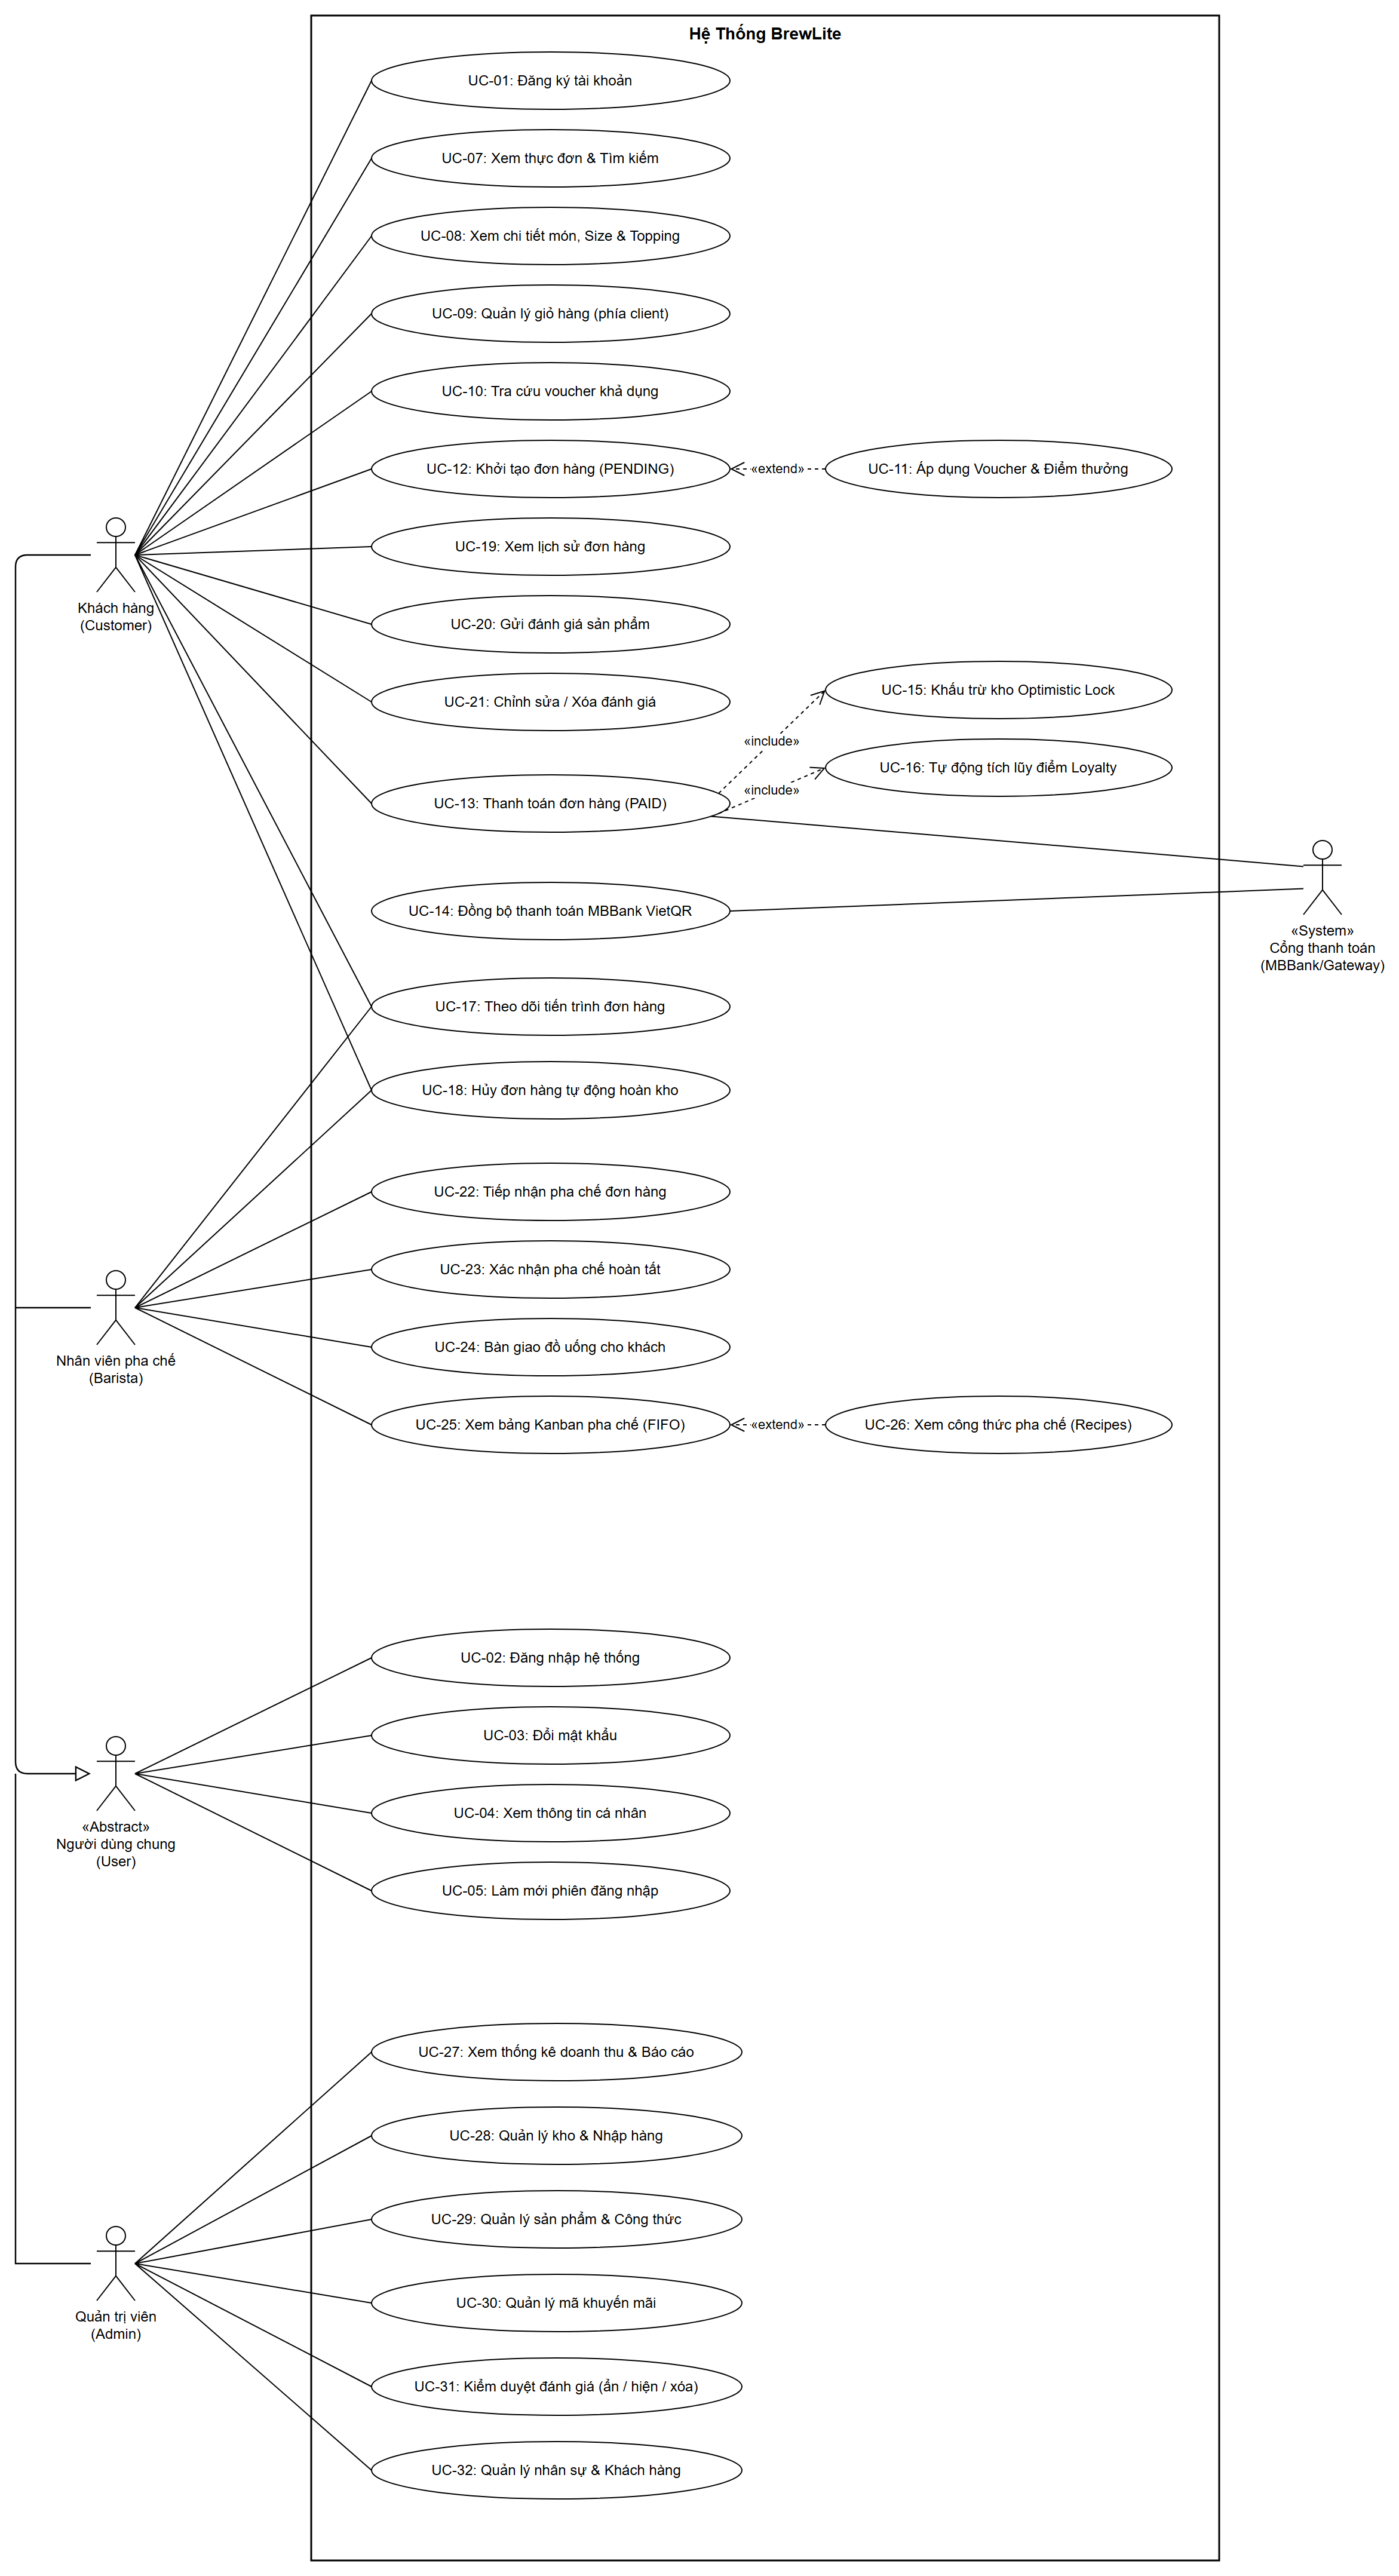
\includegraphics[width=1.08\textwidth,height=0.92\textheight,keepaspectratio]{img/Usecase_cnpm_01.drawio.png}%
}
\caption{Sơ đồ Use-case toàn hệ thống BrewLite}
\label{fig:uc-overall}
\end{figure}

Qua sơ đồ Hình 1.1 có thể thấy sự phân công chức năng giữa các tác nhân là rõ ràng và không chồng chéo. Khách hàng thực hiện toàn bộ quy trình tự phục vụ: đăng ký tài khoản (UC-01), xem thực đơn và tìm kiếm (UC-07), xem chi tiết món (UC-08), quản lý giỏ hàng (UC-09), tra cứu voucher khả dụng (UC-10), khởi tạo đơn hàng (UC-12, mở rộng bởi UC-11 Áp dụng Voucher \& Điểm thưởng), thanh toán đơn hàng (UC-13), theo dõi tiến trình đơn hàng (UC-17), hủy đơn hàng (UC-18), xem lịch sử đơn hàng (UC-19), gửi đánh giá sản phẩm đã mua (UC-20) và chỉnh sửa/xóa đánh giá (UC-21). Nhân viên pha chế tập trung vào nghiệp vụ tại quầy: tiếp nhận pha chế (UC-22), xác nhận pha chế hoàn tất (UC-23), bàn giao đồ uống cho khách (UC-24), xem bảng Kanban pha chế (UC-25, mở rộng bởi UC-26 Xem công thức pha chế). Cổng thanh toán tham gia vào Use-case Thanh toán đơn hàng (UC-13) và Đồng bộ thanh toán MBBank VietQR (UC-14). Quản trị viên thực hiện 6 nhóm chức năng quản trị (UC-27 đến UC-32): xem thống kê doanh thu \& báo cáo, quản lý kho \& nhập hàng, quản lý sản phẩm \& công thức, quản lý mã khuyến mãi, kiểm duyệt đánh giá khách hàng và quản lý nhân sự \& khách hàng. Các Use-case Đăng nhập (UC-02), Đổi mật khẩu (UC-03), Xem thông tin cá nhân (UC-04), Làm mới phiên đăng nhập (UC-05) và Đăng xuất (UC-06) thuộc về tác nhân trừu tượng Người dùng chung (User); cả Khách hàng, Nhân viên pha chế và Quản trị viên đều kế thừa các Use-case này từ User. Phân công tác nhân -- Use-case được tổng hợp trong Bảng 1.6.

\begin{longtable}{>{\raggedright\arraybackslash}p{3.4cm}>{\raggedright\arraybackslash}p{11.8cm}}
\caption{Phân công Use-case theo tác nhân}\\
\hline
\rowcolor{gray!20} \textbf{Tác nhân} & \textbf{Các Use-case đảm nhiệm} \\
\hline
\endfirsthead
\hline
\rowcolor{gray!20} \textbf{Tác nhân} & \textbf{Các Use-case đảm nhiệm} \\
\hline
\endhead
Khách hàng (Customer) & UC-01 Đăng ký tài khoản; UC-07 Xem thực đơn \& Tìm kiếm; UC-08 Xem chi tiết món, Size \& Topping; UC-09 Quản lý giỏ hàng; UC-10 Tra cứu voucher khả dụng; UC-11 Áp dụng Voucher \& Điểm thưởng; UC-12 Khởi tạo đơn hàng (PENDING); UC-13 Thanh toán đơn hàng (PAID); UC-17 Theo dõi tiến trình đơn hàng; UC-18 Hủy đơn hàng tự động hoàn kho; UC-19 Xem lịch sử đơn hàng; UC-20 Gửi đánh giá sản phẩm đã mua; UC-21 Chỉnh sửa / Xóa đánh giá; kế thừa từ User: UC-02 Đăng nhập, UC-03 Đổi mật khẩu, UC-04 Xem thông tin cá nhân, UC-05 Làm mới phiên đăng nhập, UC-06 Đăng xuất. \\
\hline
Nhân viên pha chế (Barista) & UC-22 Tiếp nhận pha chế đơn hàng (PAID $\rightarrow$ PREPARING); UC-23 Xác nhận pha chế hoàn tất (PREPARING $\rightarrow$ READY); UC-24 Bàn giao đồ uống cho khách (READY $\rightarrow$ COMPLETED); UC-25 Xem bảng Kanban pha chế (FIFO); UC-26 Xem công thức pha chế (Recipes); kế thừa từ User: UC-02 đến UC-06. \\
\hline
Quản trị viên (Admin) & UC-27 Xem thống kê doanh thu \& Báo cáo; UC-28 Quản lý kho \& Nhập hàng; UC-29 Quản lý sản phẩm \& Công thức; UC-30 Quản lý mã khuyến mãi; UC-31 Kiểm duyệt đánh giá khách hàng; UC-32 Quản lý nhân sự \& Khách hàng; kế thừa từ User: UC-02 đến UC-06. \\
\hline
Cổng thanh toán (Payment Gateway) & UC-13 Thanh toán đơn hàng (PAID): tiếp nhận và xử lý giao dịch thanh toán; UC-14 Đồng bộ thanh toán MBBank VietQR. \\
\hline
Người dùng chung (User, \guillemotleft{}Abstract\guillemotright{}) & UC-02 Đăng nhập hệ thống; UC-03 Đổi mật khẩu; UC-04 Xem thông tin cá nhân; UC-05 Làm mới phiên đăng nhập; UC-06 Đăng xuất. Tác nhân trừu tượng: Khách hàng, Nhân viên pha chế và Quản trị viên kế thừa các Use-case này. \\
\hline
Hệ thống (nội bộ Hình 1.2--1.5) & UC-15 Khấu trừ kho Optimistic Lock (trừ nguyên liệu với cột \texttt{version} chống bán âm); UC-16 Tự động tích lũy điểm Loyalty (+1đ / 10.000đ khi PAID); cùng các bước nội bộ \guillemotleft{}include\guillemotright{}: Ghi nhận lịch sử OrderStatusHistory, Kiểm tra điều kiện đã mua món (KiemTraDaMua), Tự động hoàn kho \& Điểm thưởng. \\
\hline
\end{longtable}

Về quan hệ giữa các Use-case, sơ đồ sử dụng hai quan hệ chuẩn của UML. Quan hệ \guillemotleft{}extend\guillemotright{} thể hiện chức năng mở rộng có điều kiện: Áp dụng Voucher \& Điểm thưởng (UC-11) mở rộng cho Khởi tạo đơn hàng (UC-12), và Xem công thức pha chế (UC-26) mở rộng cho Xem bảng Kanban pha chế (UC-25). Quan hệ \guillemotleft{}include\guillemotright{} thể hiện các bước bắt buộc được kích hoạt tự động: Thanh toán đơn hàng (UC-13) \guillemotleft{}include\guillemotright{} Khấu trừ kho Optimistic Lock (UC-15) và Tự động tích lũy điểm Loyalty (UC-16) ngay trên Hình 1.1; đồng thời các sơ đồ phân hệ chi tiết (Hình 1.2--1.5) làm rõ thêm việc ghi nhận lịch sử OrderStatusHistory và kiểm tra điều kiện đã mua món (KiemTraDaMua).

\subsection{Danh sách các Use-case của hệ thống}

Để thuận tiện cho việc đặc tả chi tiết, kiểm thử và truy vết yêu cầu ở các giai đoạn sau, toàn bộ 32 Use-case của hệ thống BrewLite trên Hình 1.1 được đánh mã thống nhất từ UC-01 đến UC-32 và tổng hợp trong Bảng 1.7.

\begin{longtable}{>{\raggedright\arraybackslash}p{1.6cm}>{\raggedright\arraybackslash}p{3.9cm}>{\raggedright\arraybackslash}p{2.7cm}>{\raggedright\arraybackslash}p{6.8cm}}
\caption{Danh sách các Use-case của hệ thống BrewLite}\\
\hline
\rowcolor{gray!20} \textbf{Mã UC} & \textbf{Tên Use-case} & \textbf{Tác nhân chính} & \textbf{Mô tả tóm tắt} \\
\hline
\endfirsthead
\hline
\rowcolor{gray!20} \textbf{Mã UC} & \textbf{Tên Use-case} & \textbf{Tác nhân chính} & \textbf{Mô tả tóm tắt} \\
\hline
\endhead
UC-01 & Đăng ký tài khoản & Customer & Khách hàng tạo tài khoản mới bằng tên đăng nhập (username), họ tên, email và mật khẩu để đặt hàng, theo dõi đơn và tích điểm. \\
\hline
UC-02 & Đăng nhập hệ thống & User (Customer, Barista, Admin) & Xác thực tài khoản và cấp phát JWT Token kèm quyền truy cập theo vai trò (Customer, Barista hoặc Admin). \\
\hline
UC-03 & Đổi mật khẩu & User (Customer, Barista, Admin) & Người dùng đã đăng nhập thay đổi mật khẩu của mình sau khi xác thực đúng mật khẩu hiện tại. \\
\hline
UC-04 & Xem thông tin cá nhân & User (Customer, Barista, Admin) & Người dùng xem thông tin hồ sơ tài khoản (username, họ tên, email, vai trò; riêng Customer xem thêm điểm tích lũy). \\
\hline
UC-05 & Làm mới phiên đăng nhập & User (Customer, Barista, Admin) & Hệ thống tự động cấp lại Access Token bằng Refresh Token khi phiên hết hạn mà không yêu cầu đăng nhập lại. \\
\hline
UC-06 & Đăng xuất & User (Customer, Barista, Admin) & Người dùng kết thúc phiên đăng nhập hiện tại và xóa thông tin xác thực trên trình duyệt. \\
\hline
UC-07 & Xem thực đơn \& Tìm kiếm & Customer & Khách hàng xem danh sách đồ uống theo danh mục, tìm kiếm theo tên, xem giá cơ bản và trạng thái còn/hết hàng. \\
\hline
UC-08 & Xem chi tiết món, Size \& Topping & Customer & Khách hàng xem mô tả, đánh giá món và tùy chọn kích cỡ (S/M/L), topping, mức đường, mức đá trước khi thêm vào giỏ. \\
\hline
UC-09 & Quản lý giỏ hàng & Customer & Khách hàng thêm món vào giỏ kèm tùy chọn, tăng/giảm số lượng, xóa món; hỗ trợ mua $N$ ly với các topping khác nhau vào cùng một giỏ hàng. \\
\hline
UC-10 & Tra cứu voucher khả dụng & Customer & Khách hàng xem danh sách các mã giảm giá tại quán (không có freeship), kèm điều kiện đơn tối thiểu, mức giảm tối đa và tiến độ đạt điều kiện. \\
\hline
UC-11 & Áp dụng Voucher \& Điểm thưởng & Customer & Khách hàng chọn/nhập mã Voucher theo quy tắc đa tầng (tối đa 1 mã đơn hàng + 1 mã giờ vàng + điểm thưởng); hệ thống khóa chọn khi đơn về 0đ. \\
\hline
UC-12 & Khởi tạo đơn hàng (PENDING) & Customer & Khách hàng xác nhận giỏ hàng để tạo duy nhất một đơn hàng ở trạng thái PENDING (POST /orders) tổng hợp toàn bộ các dòng chi tiết món (OrderItems). \\
\hline
UC-13 & Thanh toán đơn hàng (PAID) & Customer, Gateway & Khách hàng thanh toán đơn PENDING qua cổng thanh toán với Idempotency-Key (POST /payments), chuyển đơn sang PAID và đảm bảo chỉ trừ tiền một lần. \\
\hline
UC-14 & Đồng bộ thanh toán MBBank VietQR & Gateway & Cổng thanh toán đồng bộ trạng thái giao dịch chuyển khoản VietQR từ MBBank về hệ thống BrewLite. \\
\hline
UC-15 & Khấu trừ kho Optimistic Lock & Hệ thống (nội bộ Hình 1.3) & Hệ thống tự động trừ nguyên liệu theo công thức khi thanh toán thành công (PAID), dùng Optimistic Locking (cột version) để chống bán âm khi đặt đồng thời. \\
\hline
UC-16 & Tự động tích lũy điểm Loyalty & Hệ thống (nội bộ Hình 1.3) & Hệ thống tự động cộng điểm thưởng (+1 điểm / 10.000đ thanh toán thực tế) cho khách hàng khi đơn chuyển sang PAID. \\
\hline
UC-17 & Theo dõi tiến trình đơn hàng & Customer & Khách hàng theo dõi tiến độ đơn hàng theo thời gian thực qua máy trạng thái (GET /orders/:id) từ PENDING đến COMPLETED. \\
\hline
UC-18 & Hủy đơn hàng tự động hoàn kho & Customer & Khách hàng hủy đơn khi ở trạng thái PENDING hoặc PAID (chặn từ PREPARING trở đi); nếu đơn đã PAID sẽ tự động hoàn kho nguyên liệu theo định lượng công thức, hoàn tiền và thu hồi điểm loyalty. \\
\hline
UC-19 & Xem lịch sử đơn hàng & Customer & Khách hàng xem danh sách các hóa đơn đã đặt (GET /orders/me), hiển thị tổng số ly, tóm tắt các món và xem chi tiết hóa đơn dòng món (OrderItems). \\
\hline
UC-20 & Gửi đánh giá sản phẩm đã mua & Customer & Khách hàng đánh giá 1--5 sao kèm nhận xét cho món thuộc đơn đã hoàn thành (COMPLETED) qua POST /reviews. \\
\hline
UC-21 & Chỉnh sửa / Xóa đánh giá & Customer & Khách hàng chỉnh sửa nội dung, số sao hoặc xóa đánh giá của chính mình (PATCH / DELETE /reviews/:id). \\
\hline
UC-22 & Tiếp nhận pha chế đơn hàng & Barista & Nhân viên pha chế tiếp nhận đơn đã thanh toán, chuyển trạng thái PAID $\rightarrow$ PREPARING (POST /staff/orders/:id/accept) kèm ghi vết OrderStatusHistory. \\
\hline
UC-23 & Xác nhận pha chế hoàn tất & Barista & Nhân viên pha chế xác nhận hoàn tất pha chế, chuyển trạng thái PREPARING $\rightarrow$ READY (POST /staff/orders/:id/ready). \\
\hline
UC-24 & Bàn giao đồ uống cho khách & Barista & Nhân viên pha chế xác nhận đã giao món cho khách, chuyển trạng thái READY $\rightarrow$ COMPLETED (POST /staff/orders/:id/complete). \\
\hline
UC-25 & Xem bảng Kanban pha chế (FIFO) & Barista & Nhân viên pha chế xem danh sách đơn cần xử lý sắp xếp theo thứ tự thời gian đặt (createdAt tăng dần) trên bảng Kanban. \\
\hline
UC-26 & Xem công thức pha chế (Recipes) & Barista & Nhân viên pha chế xem định lượng nguyên liệu chi tiết cho từng ly của đơn hàng (GET /staff/orders/:id/recipes). \\
\hline
UC-27 & Xem thống kê doanh thu \& Báo cáo & Admin & Quản trị viên xem tổng quan doanh thu, biểu đồ theo thời gian, top sản phẩm bán chạy và thống kê trạng thái đơn hàng. \\
\hline
UC-28 & Quản lý kho \& Nhập hàng & Admin & Quản trị viên quản lý tồn kho nguyên liệu, cảnh báo sắp hết hàng, quản lý nhà cung cấp và lập phiếu nhập kho. \\
\hline
UC-29 & Quản lý sản phẩm \& Công thức & Admin & Quản trị viên thêm/sửa/xóa món đồ uống, biến thể kích cỡ (S/M/L) và thiết lập công thức định lượng nguyên liệu. \\
\hline
UC-30 & Quản lý mã khuyến mãi & Admin & Quản trị viên tạo mới, chỉnh sửa, xóa và quản lý điều kiện áp dụng các mã Voucher giảm giá. \\
\hline
UC-31 & Kiểm duyệt đánh giá khách hàng & Admin & Quản trị viên xem danh sách toàn bộ đánh giá và thực hiện ẩn hoặc hiện lại các đánh giá của khách hàng. \\
\hline
UC-32 & Quản lý nhân sự \& Khách hàng & Admin & Quản trị viên tạo/sửa/xóa tài khoản Barista, quản lý khách hàng và thực hiện khóa hoặc mở khóa tài khoản. \\
\hline
\end{longtable}

\subsection{Sơ đồ Use-case riêng và đặc tả Use-case}

Trên cơ sở sơ đồ Use-case toàn hệ thống, nhóm thực hiện tiếp tục phân rã các luồng nghiệp vụ trọng tâm thành bốn sơ đồ Use-case riêng (Hình 1.2 đến Hình 1.5) cho các phân hệ khách hàng và quầy pha chế, còn các Use-case quản trị (UC-27 đến UC-32) được thể hiện trực tiếp trên Hình 1.1 và Bảng 1.7. Mỗi bảng đặc tả dưới đây gồm các thành phần: mã Use-case (Use Case ID), tên Use-case, tác nhân, liên kết yêu cầu, tóm tắt, tiền điều kiện, hậu điều kiện, dòng sự kiện chính và dòng sự kiện phụ.

\subsubsection*{a. Phân hệ Tài khoản, thực đơn \& giỏ hàng}

Phân hệ Tài khoản, thực đơn \& giỏ hàng bao gồm các Use-case trải nghiệm mua hàng ban đầu của Khách hàng trên sơ đồ toàn hệ thống: Đăng ký tài khoản (UC-01), Xem thực đơn \& Tìm kiếm (UC-07), Xem chi tiết món, Size \& Topping (UC-08) và Quản lý giỏ hàng (UC-09). Các Use-case Đăng nhập hệ thống (UC-02), Đổi mật khẩu (UC-03), Xem thông tin cá nhân (UC-04), Làm mới phiên đăng nhập (UC-05) và Đăng xuất (UC-06) thuộc về tác nhân trừu tượng Người dùng chung (User) mà Khách hàng, Nhân viên pha chế và Quản trị viên đều kế thừa.

\begin{figure}[!htbp]
\centering
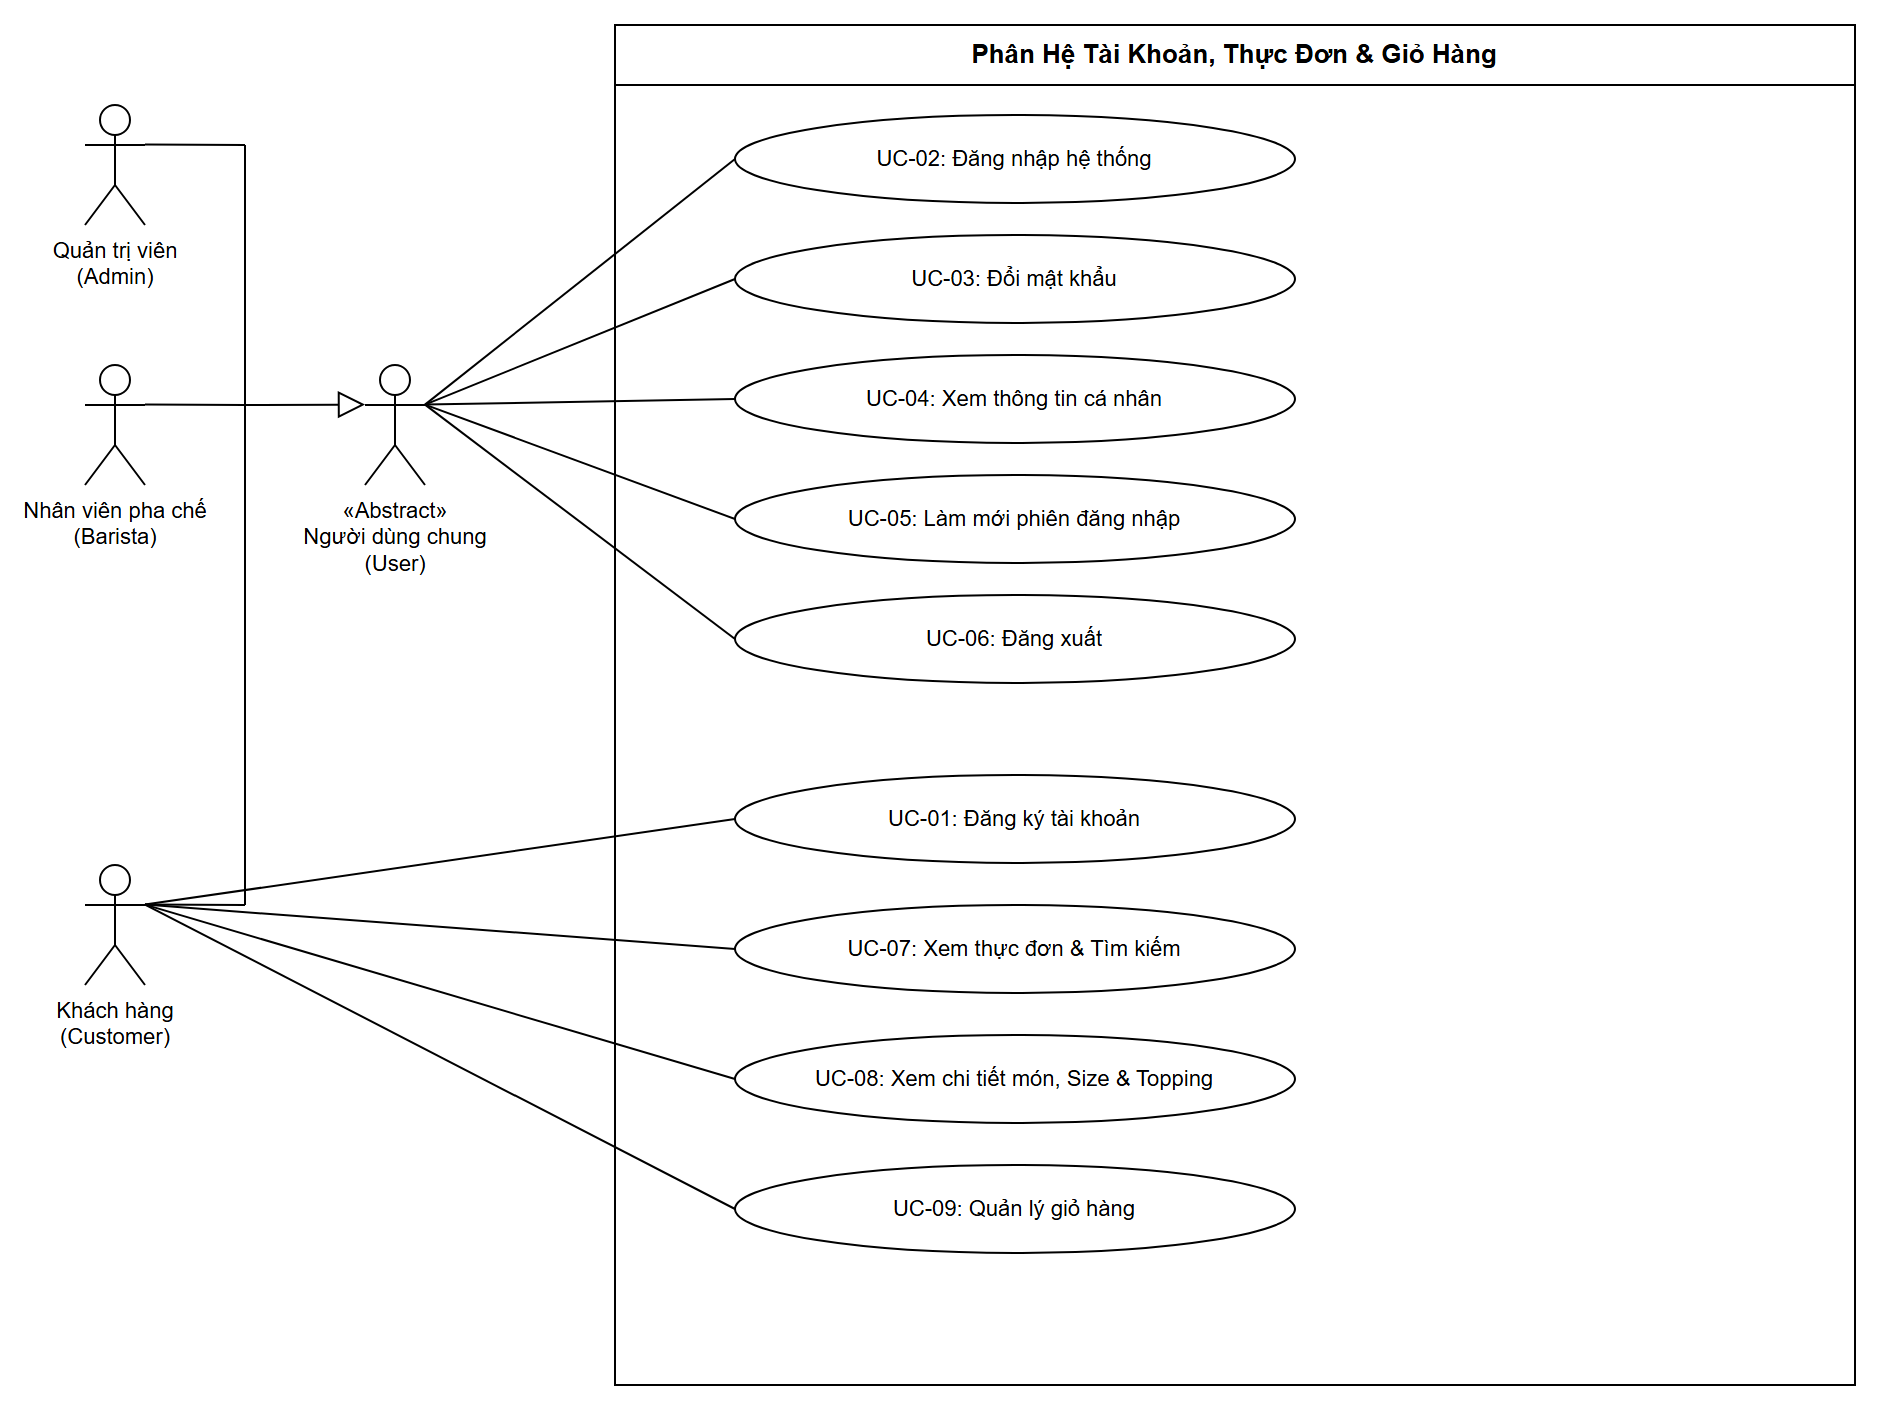
\includegraphics[width=\textwidth]{img/Usecase_cnpm_02.drawio.png}
\caption{Sơ đồ Use-case Phân hệ Tài khoản, thực đơn \& giỏ hàng}
\label{fig:uc-account-menu-cart}
\end{figure}

\subsubsection*{b. Phân hệ Đặt hàng \& Thanh toán đồng thời}

Phân hệ Đặt hàng \& Thanh toán đồng thời có hai tác nhân là Khách hàng (Customer) và Cổng thanh toán (Payment Gateway). Khách hàng tra cứu voucher khả dụng (UC-10) và thực hiện Khởi tạo đơn hàng PENDING (UC-12, POST /orders); Use-case này được mở rộng (\guillemotleft{}extend\guillemotright{}) bởi Áp dụng Voucher \& Điểm thưởng (UC-11, POST /promotions/validate) và \guillemotleft{}include\guillemotright{} Ghi nhận lịch sử OrderStatusHistory. Khách hàng và Cổng thanh toán cùng thực hiện Thanh toán đơn hàng (UC-13, POST /payments + Idempotency-Key); Use-case này \guillemotleft{}include\guillemotright{} Khấu trừ kho Optimistic Lock (UC-15), Tự động tích lũy điểm Loyalty (UC-16, +1đ / 10.000đ khi PAID) và Ghi nhận lịch sử OrderStatusHistory (PENDING $\rightarrow$ PAID). Đồng thời, Khách hàng có quyền thực hiện Hủy đơn hàng tự động hoàn kho (UC-18, POST /orders/:id/cancel) khi đơn còn ở trạng thái PENDING hoặc PAID (hệ thống chặn hủy từ PREPARING trở đi để bảo vệ chi phí pha chế); Use-case hủy đơn \guillemotleft{}include\guillemotright{} Tự động hoàn kho \& Điểm thưởng và Ghi vết lịch sử hủy đơn (OrderStatusHistory). Cổng thanh toán thực hiện Đồng bộ thanh toán MBBank VietQR (UC-14).

\begin{figure}[!htbp]
\centering
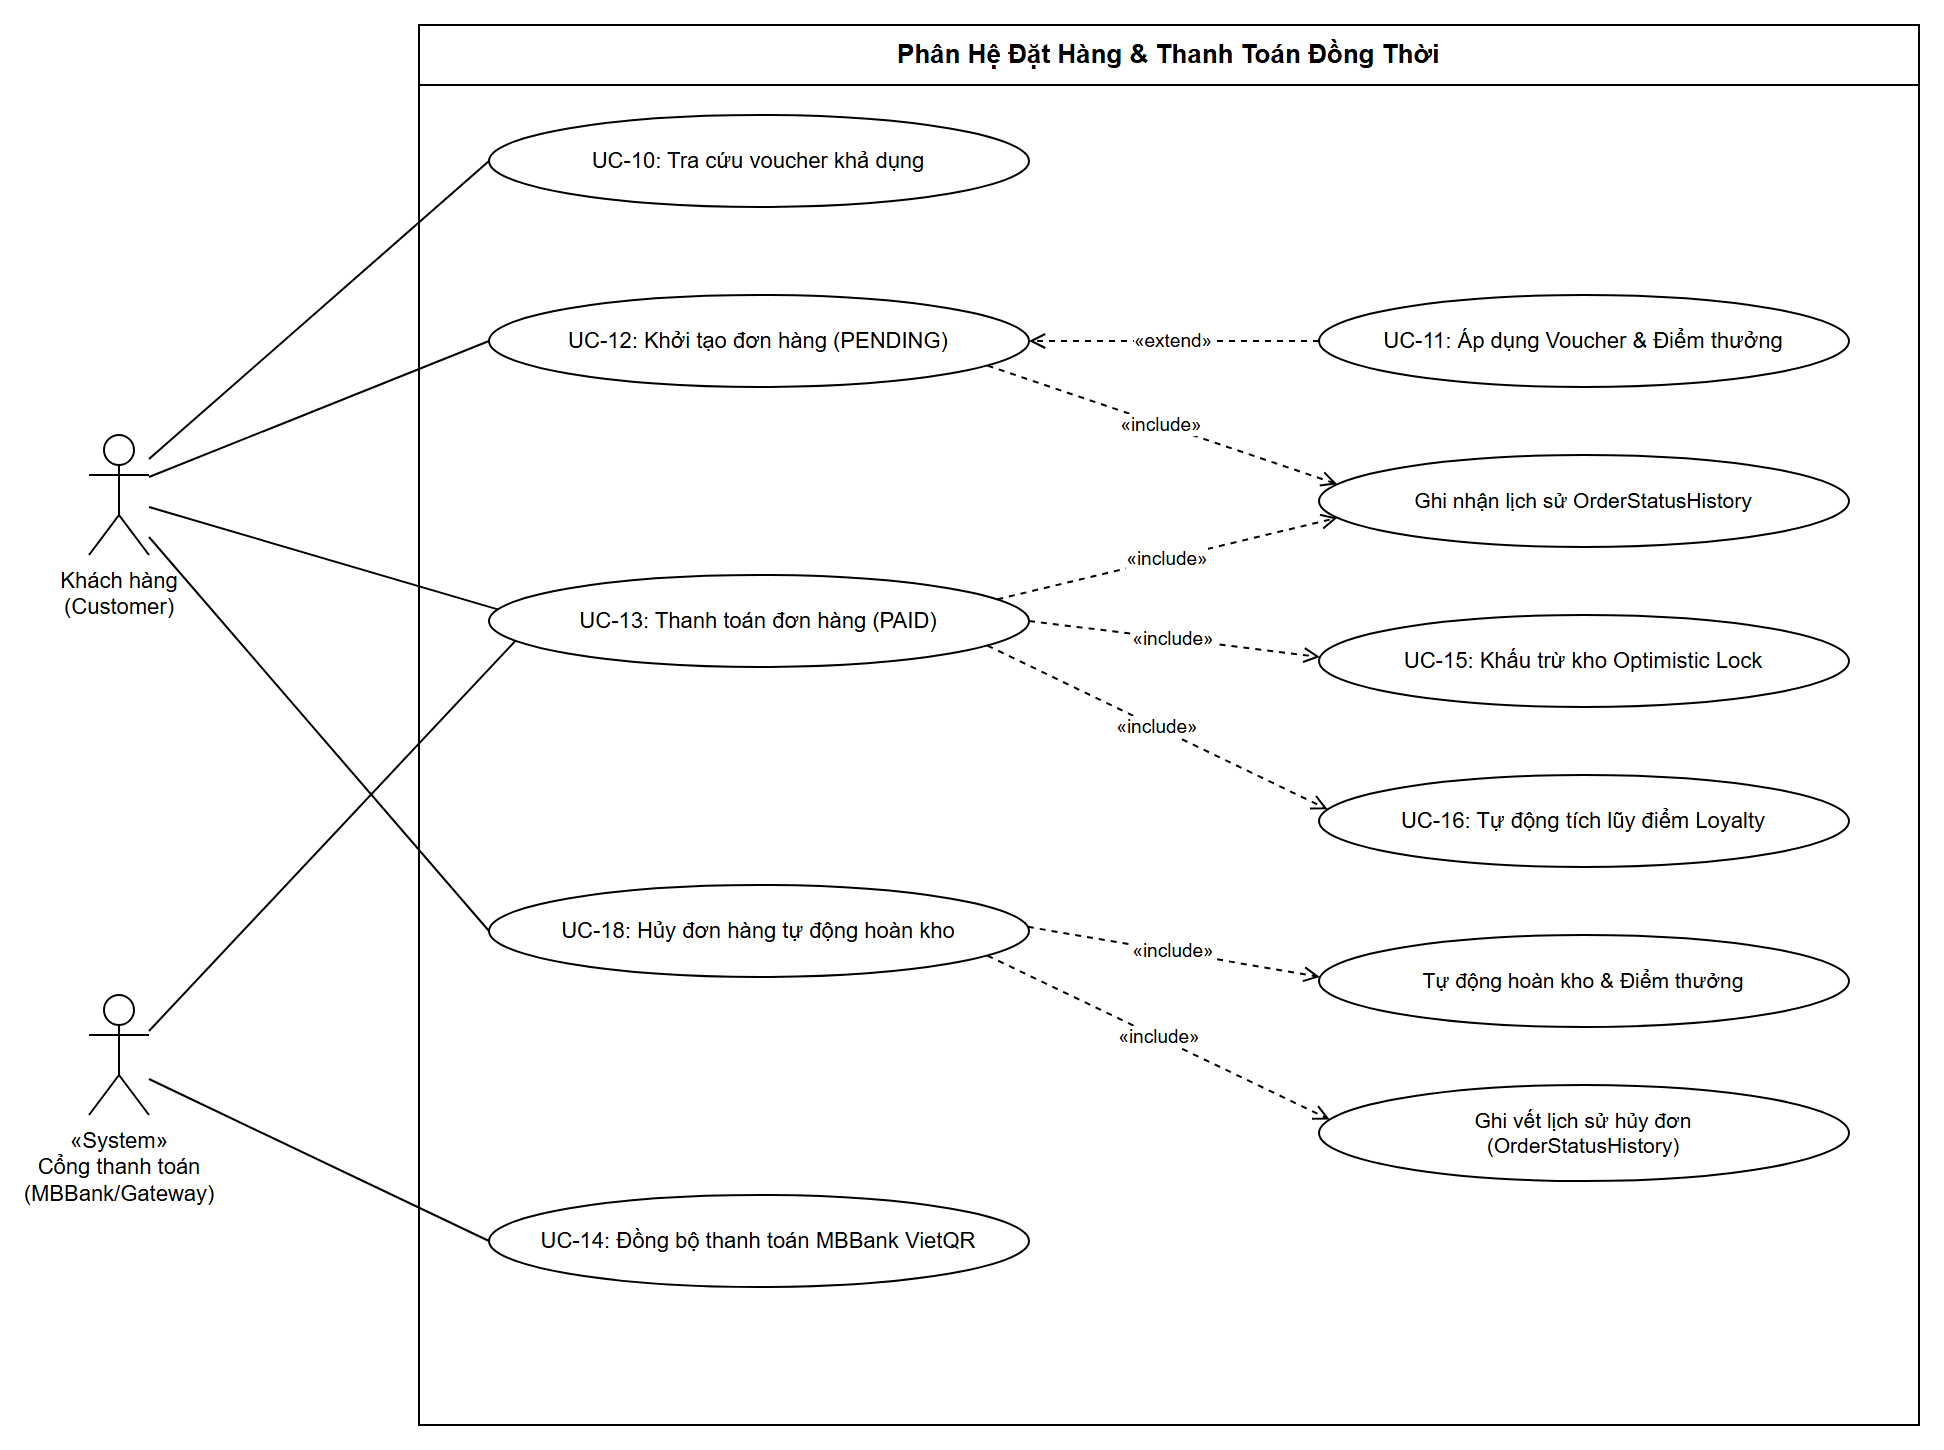
\includegraphics[width=\textwidth]{img/Usecase_cnpm_03.drawio.png}
\caption{Sơ đồ Use-case Phân hệ Đặt hàng \& Thanh toán đồng thời}
\label{fig:uc-order-payment}
\end{figure}

\subsubsection*{c. Phân hệ Quầy pha chế \& Máy trạng thái}

Phân hệ Quầy pha chế \& Máy trạng thái có tác nhân chính là Nhân viên pha chế (Barista). Nhân viên pha chế xem bảng Kanban pha chế theo FIFO (UC-25, GET /staff/orders); Use-case này được mở rộng (\guillemotleft{}extend\guillemotright{}) bởi Xem công thức pha chế chi tiết từng ly (UC-26, GET /staff/orders/:id/recipes). Tiếp nhận pha chế đơn hàng (UC-22, PAID $\rightarrow$ PREPARING, POST /staff/orders/:id/accept), Xác nhận pha chế hoàn tất (UC-23, PREPARING $\rightarrow$ READY, POST /staff/orders/:id/ready) và Bàn giao đồ uống cho khách (UC-24, READY $\rightarrow$ COMPLETED, POST /staff/orders/:id/complete) đều \guillemotleft{}include\guillemotright{} Ghi vết kiểm toán trạng thái (OrderStatusHistory).

\begin{figure}[!htbp]
\centering
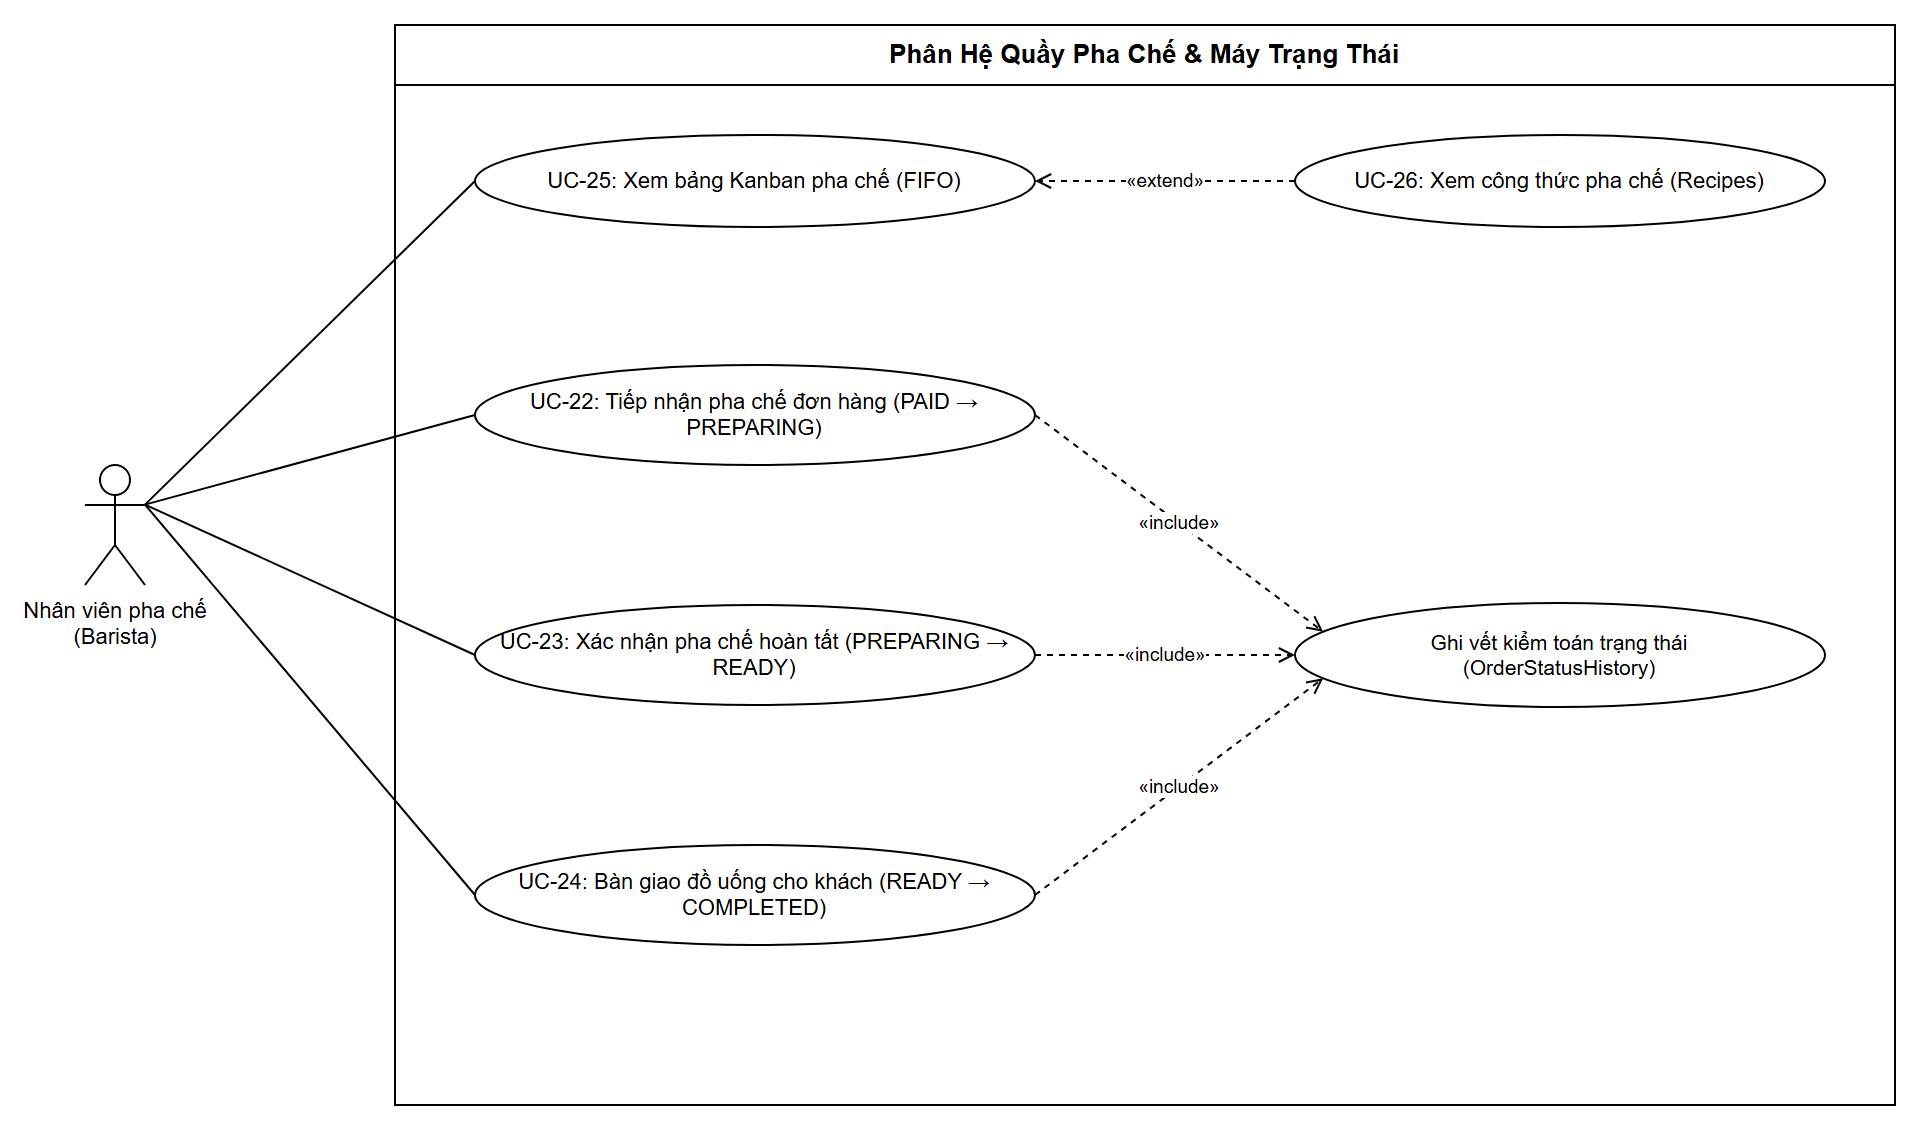
\includegraphics[width=\textwidth]{img/Usecase_cnpm_04.drawio.png}
\caption{Sơ đồ Use-case Phân hệ Quầy pha chế \& Máy trạng thái}
\label{fig:uc-barista}
\end{figure}

\subsubsection*{d. Phân hệ Đánh giá sản phẩm \& Lịch sử}

Phân hệ Đánh giá sản phẩm \& Lịch sử có tác nhân là Khách hàng (Customer). Khách hàng Theo dõi tiến trình đơn hàng (UC-17, GET /orders/:id) và Hủy đơn hàng tự động hoàn kho (UC-18, POST /orders/:id/cancel, chặn khi PREPARING); Use-case hủy đơn \guillemotleft{}include\guillemotright{} Tự động hoàn kho \& Điểm thưởng và Ghi vết lịch sử hủy đơn (OrderStatusHistory). Khách hàng Xem lịch sử đơn hàng (UC-19, GET /orders/me), Gửi đánh giá sản phẩm đã mua (UC-20, 1--5 sao \& Nhận xét, POST /reviews) và Chỉnh sửa / Xóa đánh giá (UC-21, PATCH / DELETE /reviews/:id). Use-case Gửi đánh giá \guillemotleft{}include\guillemotright{} Kiểm tra điều kiện đã mua món (KiemTraDaMua), bảo đảm chỉ món thuộc đơn đã COMPLETED mới được đánh giá.

\begin{figure}[!htbp]
\centering
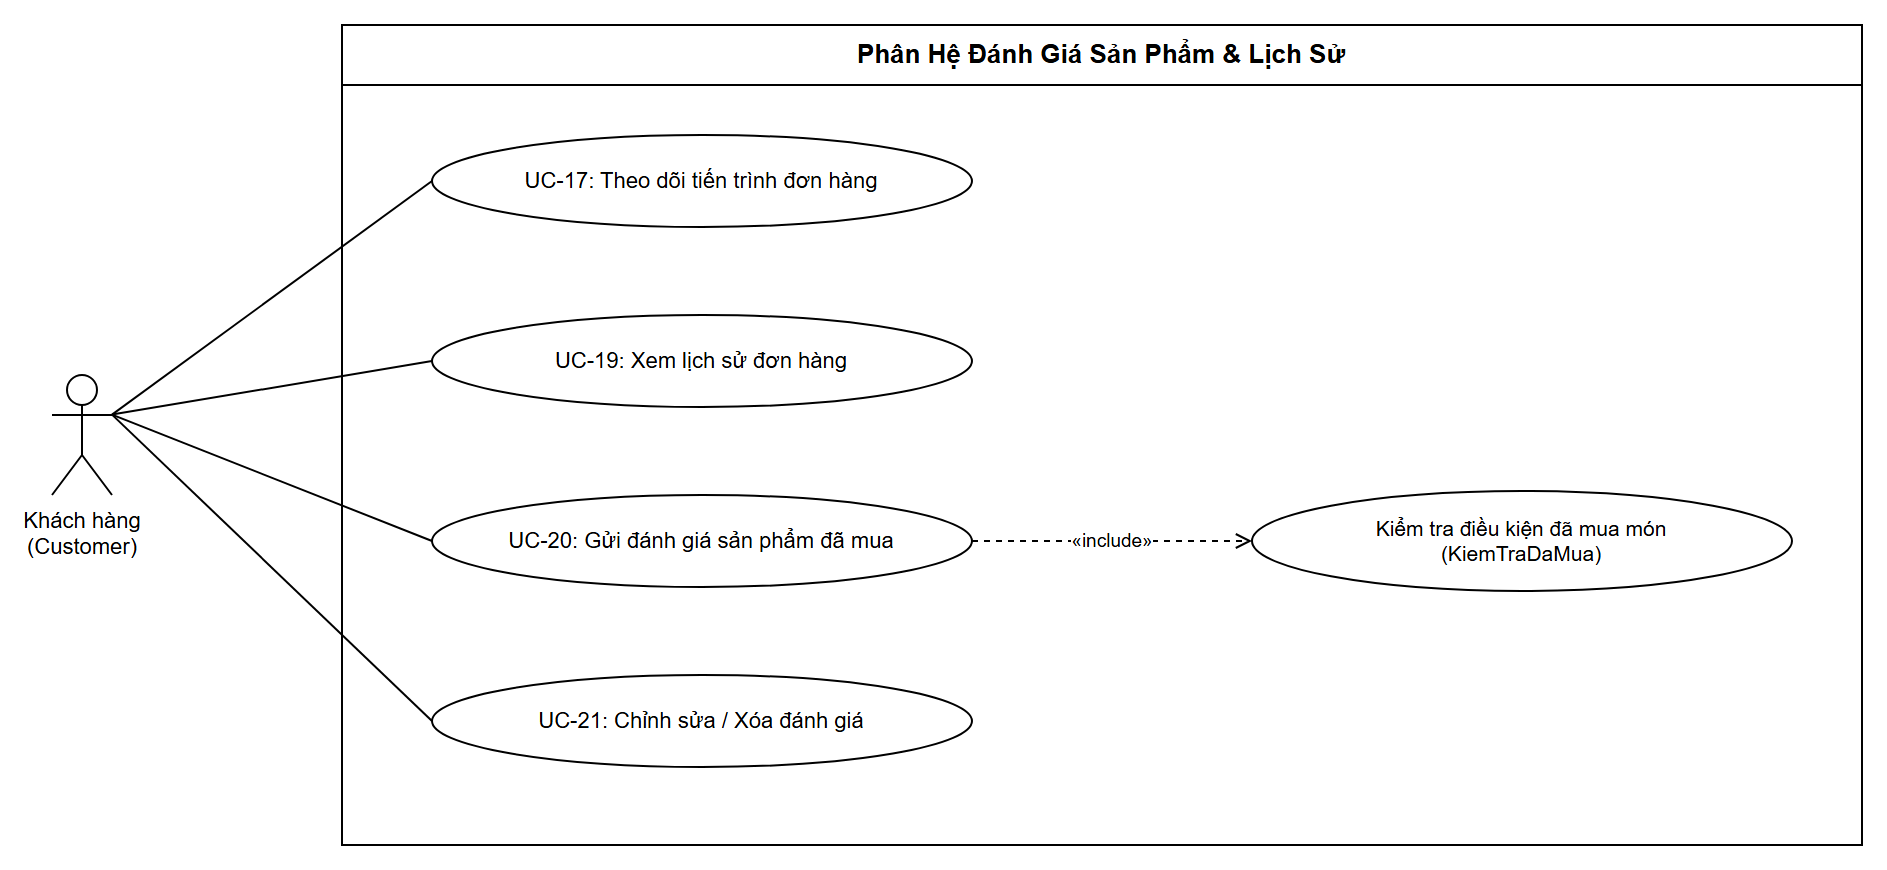
\includegraphics[width=\textwidth]{img/Usecase_cnpm_05.drawio.png}
\caption{Sơ đồ Use-case Phân hệ Đánh giá sản phẩm \& Lịch sử}
\label{fig:uc-review-history}
\end{figure}

\subsubsection*{e. Đặc tả chi tiết Use-case}

Dưới đây là đặc tả chi tiết của các Use-case cốt lõi theo mã Use-case mới trong Bảng 1.7: Thanh toán đơn hàng Idempotent (UC-13), Gửi đánh giá sản phẩm đã mua (UC-20), Xem bảng Kanban pha chế (UC-25), Xem chi tiết đơn hàng (luồng chi tiết của UC-25), Xem công thức pha chế chi tiết (UC-26) và Cập nhật trạng thái pha chế (UC-22 / UC-23 / UC-24).

\subsubsection*{Thanh toán đơn hàng chống trùng lặp (Idempotent Payment)}

\begin{longtable}{>{\raggedright\arraybackslash}p{3.8cm}>{\raggedright\arraybackslash}p{11.4cm}}
\hline
\cellcolor{blue!10}\textbf{Use Case ID} & UC-13 \\
\hline
\cellcolor{blue!10}\textbf{Tên Use Case} & Thanh toán đơn hàng (PAID) -- Idempotent Payment \\
\hline
\cellcolor{blue!10}\textbf{Tác nhân} & Khách hàng (Customer) \& Cổng thanh toán (Payment Gateway) \\
\hline
\cellcolor{blue!10}\textbf{Liên kết yêu cầu} & FR-07 (Thanh toán Idempotent), FR-09 (Kiểm soát tồn kho OCC), NFR-01 (Hiệu năng), NFR-04 (Toàn vẹn ACID) \\
\hline
\cellcolor{blue!10}\textbf{Tóm tắt} & Cho phép khách hàng thanh toán đơn hàng ở trạng thái PENDING hoặc PAYMENT\_FAILED qua cổng thanh toán (Ví/Thẻ/VietQR MBBank). Mỗi yêu cầu thanh toán mang một Idempotency-Key duy nhất, bảo đảm hệ thống chỉ trừ tiền và chuyển đơn sang PAID một lần duy nhất dù khách gửi lại yêu cầu hoặc bấm đúp. \\
\hline
\cellcolor{blue!10}\textbf{Tiền điều kiện} & -- Khách hàng đã đăng nhập (UC-02). \newline
-- Đơn hàng thuộc về khách hàng và đang ở trạng thái PENDING hoặc PAYMENT\_FAILED. \newline
-- Đơn hàng đã được tính tổng cuối cùng sau khi áp dụng Voucher và điểm thưởng (UC-11). \newline
-- Cổng thanh toán sẵn sàng xử lý giao dịch. \\
\hline
\cellcolor{blue!10}\textbf{Hậu điều kiện} & -- Giao dịch thanh toán được ghi nhận duy nhất cho đơn hàng. \newline
-- Đơn hàng chuyển sang PAID và được ghi vết vào lịch sử OrderStatusHistory. \newline
-- Tồn kho nguyên liệu được khấu trừ an toàn (UC-15) và điểm thưởng được tự động cộng (+1đ / 10.000đ) cho khách hàng (UC-16). \newline
-- Khách hàng nhận được xác nhận thanh toán thành công. \\
\hline
\cellcolor{blue!10}\textbf{Dòng sự kiện chính} & 1. Khách hàng xác nhận thanh toán cho đơn hàng PENDING. \newline
2. Giao diện (UI) tự động tạo Idempotency-Key (UUIDv4) gắn vào Header và gửi yêu cầu thanh toán đến backend (POST /api/payments), backend chuyển tiếp sang Payment Service. \newline
3. Cổng thanh toán xử lý giao dịch và trả kết quả về hệ thống. \newline
4. Payment Service tra cứu giao dịch theo Idempotency-Key: nếu key đã tồn tại thì trả ngay kết quả cũ (Idempotency Replay), không trừ tiền lần hai; nếu chưa tồn tại thì kiểm tra máy trạng thái (assertTransition: chỉ cho phép PENDING hoặc PAYMENT\_FAILED sang PAID). \newline
5. Nếu thanh toán thành công: trong một ACID Transaction, hệ thống gọi cổng thanh toán mô phỏng (mockGateway.processCharge), ghi nhận giao dịch, chuyển đơn sang PAID, khấu trừ tồn kho bằng OCC (UC-15), cộng điểm thưởng (UC-16) và ghi vết OrderStatusHistory. \newline
6. Hệ thống hiển thị xác nhận thanh toán thành công cho khách hàng. \\
\hline
\cellcolor{blue!10}\textbf{Dòng sự kiện phụ} & -- Gửi lại yêu cầu với cùng Idempotency-Key (khách bấm đúp): hệ thống trả về kết quả của giao dịch gốc (HTTP 200 OK, cached: true, replayed: true), không trừ tiền và không trừ kho lần thứ hai. \newline
-- Thanh toán bị từ chối hoặc thất bại: đơn hàng chuyển sang trạng thái PAYMENT\_FAILED, hệ thống thông báo lý do và khách hàng có thể thử thanh toán lại. \newline
-- Hết nguyên liệu hoặc xung đột phiên bản (OCC retry thất bại): hệ thống rollback giao dịch và trả về HTTP 409 Conflict. \\
\hline
\end{longtable}

\subsubsection*{Đánh giá chất lượng đồ uống đã mua}

\begin{longtable}{>{\raggedright\arraybackslash}p{3.8cm}>{\raggedright\arraybackslash}p{11.4cm}}
\hline
\cellcolor{blue!10}\textbf{Use Case ID} & UC-20 \\
\hline
\cellcolor{blue!10}\textbf{Tên Use Case} & Gửi đánh giá sản phẩm đã mua \\
\hline
\cellcolor{blue!10}\textbf{Tác nhân} & Khách hàng (Customer) \\
\hline
\cellcolor{blue!10}\textbf{Liên kết yêu cầu} & FR-12 (Đánh giá đồ uống đã mua) \\
\hline
\cellcolor{blue!10}\textbf{Tóm tắt} & Cho phép khách hàng đánh giá chất lượng đồ uống đã mua bằng mức 1--5 sao kèm nhận xét (POST /reviews). Điều kiện bắt buộc: chỉ món thuộc đơn hàng mà khách hàng đã mua (đơn đã ở trạng thái COMPLETED) mới được đánh giá; điều kiện này được hệ thống kiểm tra tự động thông qua Use-case Kiểm tra điều kiện đã mua món (KiemTraDaMua). \\
\hline
\cellcolor{blue!10}\textbf{Tiền điều kiện} & -- Khách hàng đã đăng nhập (UC-02) và là chủ sở hữu của đơn hàng. \newline
-- Đơn hàng chứa món cần đánh giá đã ở trạng thái COMPLETED (khách hàng đã mua và đã nhận đồ uống). \newline
-- Món cần đánh giá thuộc đơn hàng đó. \\
\hline
\cellcolor{blue!10}\textbf{Hậu điều kiện} & -- Đánh giá được lưu và gắn với món, đơn hàng và khách hàng; điểm trung bình của món được cập nhật. \newline
-- Khách hàng có thể xem, sửa hoặc xóa đánh giá của mình. \\
\hline
\cellcolor{blue!10}\textbf{Dòng sự kiện chính} & 1. Khách hàng mở trang chi tiết sản phẩm (UC-08) hoặc lịch sử đơn đã mua (UC-19) và chọn món cần đánh giá. \newline
2. Hệ thống kiểm tra điều kiện đã mua món (KiemTraDaMua) và hiển thị biểu mẫu đánh giá. \newline
3. Khách hàng chọn mức 1--5 sao, nhập nhận xét và nhấn ``Gửi đánh giá''. \newline
4. Hệ thống kiểm tra tính hợp lệ (mức sao trong khoảng 1--5, nội dung nhận xét không rỗng) và lưu đánh giá. \newline
5. Hệ thống hiển thị xác nhận; đánh giá được gắn cùng món để các khách hàng khác tham khảo. \\
\hline
\cellcolor{blue!10}\textbf{Dòng sự kiện phụ} & -- Món chưa được mua (đơn chưa COMPLETED hoặc món không thuộc đơn hàng của khách): hệ thống từ chối đánh giá và thông báo rõ điều kiện đã mua. \newline
-- Khách hàng đã đánh giá món này rồi: hệ thống báo lỗi xung đột (HTTP 409) và hướng dẫn dùng chức năng chỉnh sửa hoặc xóa đánh giá đã có (UC-21, PATCH / DELETE /reviews/:id). \newline
-- Mức sao ngoài khoảng 1--5: hệ thống báo lỗi và không lưu đánh giá. \newline
-- Phiên đăng nhập hết hạn: hệ thống chuyển về màn hình Đăng nhập. \\
\hline
\end{longtable}

\subsubsection*{Xem bảng Kanban đơn hàng}

\begin{longtable}{>{\raggedright\arraybackslash}p{3.8cm}>{\raggedright\arraybackslash}p{11.4cm}}
\hline
\cellcolor{blue!10}\textbf{Use Case ID} & UC-25 \\
\hline
\cellcolor{blue!10}\textbf{Tên Use Case} & Xem bảng Kanban pha chế (FIFO) \\
\hline
\cellcolor{blue!10}\textbf{Tác nhân} & Nhân viên pha chế (Barista) \\
\hline
\cellcolor{blue!10}\textbf{Liên kết yêu cầu} & FR-08 (Máy trạng thái đơn hàng) \\
\hline
\cellcolor{blue!10}\textbf{Tóm tắt} & Cho phép Nhân viên pha chế xem bảng Kanban các đơn hàng ở 3 cột trạng thái (PAID, PREPARING, READY), sắp xếp theo thứ tự FIFO (\texttt{createdAt} tăng dần) qua API GET /staff/orders, kèm mã đơn, số lượng món và thời gian đặt. Đây là điểm bắt đầu cho các thao tác tiếp nhận đơn, xem công thức pha chế và cập nhật trạng thái. \\
\hline
\cellcolor{blue!10}\textbf{Tiền điều kiện} & -- Nhân viên pha chế đã đăng nhập (UC-02) với quyền truy cập màn hình quầy pha chế (STAFF hoặc ADMIN). \newline
-- Hệ thống đang hoạt động và có kết nối đến cơ sở dữ liệu. \\
\hline
\cellcolor{blue!10}\textbf{Hậu điều kiện} & -- Bảng Kanban được hiển thị đúng thứ tự FIFO và tự động làm mới định kỳ khi có đơn mới; dữ liệu đơn hàng không bị thay đổi. \\
\hline
\cellcolor{blue!10}\textbf{Dòng sự kiện chính} & 1. Nhân viên pha chế đăng nhập và truy cập màn hình Kanban (\texttt{/staff}). \newline
2. Hệ thống tải và hiển thị danh sách đơn hàng theo 3 cột PAID, PREPARING, READY đúng thứ tự FIFO. \newline
3. Nhân viên pha chế theo dõi bảng Kanban. \newline
4. Từ bảng Kanban, Nhân viên pha chế chọn đơn để xem chi tiết thẻ đơn (UC-25), xem công thức pha chế (UC-26) hoặc cập nhật trạng thái đơn (UC-22 / UC-23 / UC-24). \\
\hline
\cellcolor{blue!10}\textbf{Dòng sự kiện phụ} & -- Không có đơn hàng nào đang chờ: cột tương ứng hiển thị trạng thái trống kèm thông báo. \newline
-- Mất kết nối mạng: hệ thống ghi nhận lỗi tải dữ liệu và thử tải lại ở chu kỳ làm mới kế tiếp. \\
\hline
\end{longtable}

\subsubsection*{Xem chi tiết đơn hàng (tại quầy pha chế)}

\begin{longtable}{>{\raggedright\arraybackslash}p{3.8cm}>{\raggedright\arraybackslash}p{11.4cm}}
\hline
\cellcolor{blue!10}\textbf{Use Case ID} & UC-25 (Luồng chi tiết đơn) \\
\hline
\cellcolor{blue!10}\textbf{Tên Use Case} & Xem chi tiết thẻ đơn hàng (thuộc UC-25) \\
\hline
\cellcolor{blue!10}\textbf{Tác nhân} & Nhân viên pha chế (Barista) \\
\hline
\cellcolor{blue!10}\textbf{Tóm tắt} & Cho phép Nhân viên pha chế xem chi tiết các món trên thẻ đơn trong bảng Kanban, gồm danh sách món, số lượng, size, topping, mã đơn, thời gian đặt và trạng thái hiện tại, phục vụ việc pha chế chính xác. Từ thẻ đơn trên bảng Kanban, Nhân viên pha chế có thể mở tiếp công thức pha chế (UC-26). \\
\hline
\cellcolor{blue!10}\textbf{Tiền điều kiện} & -- Nhân viên pha chế đã đăng nhập (UC-02). \newline
-- Đơn hàng tồn tại trong bảng Kanban. \\
\hline
\cellcolor{blue!10}\textbf{Hậu điều kiện} & -- Chi tiết đơn hàng được hiển thị đầy đủ; dữ liệu đơn hàng không bị thay đổi. \\
\hline
\cellcolor{blue!10}\textbf{Dòng sự kiện chính} & 1. Từ màn hình bảng Kanban (UC-25), Nhân viên pha chế quan sát thẻ đơn hàng cần xử lý. \newline
2. Hệ thống hiển thị chi tiết món, size, topping và số lượng. \newline
3. Nhân viên pha chế đối chiếu chi tiết món trước khi tiến hành pha chế. \newline
4. Khi cần, Nhân viên pha chế mở công thức pha chế chi tiết của đơn (UC-26). \\
\hline
\cellcolor{blue!10}\textbf{Dòng sự kiện phụ} & -- Đơn hàng vừa được Nhân viên khác cập nhật trạng thái: hệ thống làm mới dữ liệu và hiển thị trạng thái mới nhất. \newline
-- Đơn hàng không còn tồn tại: thẻ đơn biến mất khỏi bảng Kanban sau khi làm mới. \\
\hline
\end{longtable}

\subsubsection*{Xem công thức pha chế (Recipes)}

\begin{longtable}{>{\raggedright\arraybackslash}p{3.8cm}>{\raggedright\arraybackslash}p{11.4cm}}
\hline
\cellcolor{blue!10}\textbf{Use Case ID} & UC-26 \\
\hline
\cellcolor{blue!10}\textbf{Tên Use Case} & Xem công thức pha chế (Recipes) \\
\hline
\cellcolor{blue!10}\textbf{Tác nhân} & Nhân viên pha chế (Barista) \\
\hline
\cellcolor{blue!10}\textbf{Tóm tắt} & Cho phép Nhân viên pha chế xem công thức pha chế chi tiết từng ly của một đơn hàng (GET /staff/orders/:id/recipes), gồm tên nguyên liệu, định lượng và đơn vị tính, để pha chế đúng công thức chuẩn. \\
\hline
\cellcolor{blue!10}\textbf{Tiền điều kiện} & -- Nhân viên pha chế đã đăng nhập (UC-02) với quyền STAFF hoặc ADMIN. \newline
-- Đơn hàng tồn tại và đang hiển thị trên quầy pha chế. \\
\hline
\cellcolor{blue!10}\textbf{Hậu điều kiện} & -- Công thức pha chế của từng ly trong đơn được hiển thị đầy đủ; dữ liệu đơn hàng và công thức không bị thay đổi. \\
\hline
\cellcolor{blue!10}\textbf{Dòng sự kiện chính} & 1. Nhân viên pha chế đăng nhập và mở bảng Kanban (UC-25). \newline
2. Nhân viên pha chế chọn đơn hàng cần pha chế. \newline
3. Nhân viên pha chế chọn ``Xem công thức''. \newline
4. Hệ thống gọi API và hiển thị định lượng nguyên liệu cùng đơn vị tính cho từng món trong đơn. \newline
5. Nhân viên pha chế pha chế theo công thức, sau đó cập nhật trạng thái đơn (UC-22 / UC-23 / UC-24). \\
\hline
\cellcolor{blue!10}\textbf{Dòng sự kiện phụ} & -- Đơn hàng không tồn tại: hệ thống trả lỗi 404 và thông báo trên giao diện. \newline
-- Món chưa được thiết lập công thức trong hệ thống: hệ thống thông báo chưa có định lượng để báo quản lý bổ sung. \newline
-- Phiên đăng nhập hết hạn: hệ thống chuyển về màn hình Đăng nhập. \\
\hline
\end{longtable}

\subsubsection*{Cập nhật trạng thái pha chế}

\begin{longtable}{>{\raggedright\arraybackslash}p{3.8cm}>{\raggedright\arraybackslash}p{11.4cm}}
\hline
\cellcolor{blue!10}\textbf{Use Case ID} & UC-22 / UC-23 / UC-24 \\
\hline
\cellcolor{blue!10}\textbf{Tên Use Case} & Cập nhật trạng thái pha chế \\
\hline
\cellcolor{blue!10}\textbf{Tác nhân} & Nhân viên pha chế (Barista) \\
\hline
\cellcolor{blue!10}\textbf{Liên kết yêu cầu} & FR-08 (Máy trạng thái đơn hàng) \\
\hline
\cellcolor{blue!10}\textbf{Tóm tắt} & Cho phép Nhân viên pha chế cập nhật trạng thái đơn hàng theo đúng máy trạng thái của hệ thống: Tiếp nhận đơn (UC-22, PAID $\rightarrow$ PREPARING, POST /staff/orders/:id/accept), Pha chế hoàn tất (UC-23, PREPARING $\rightarrow$ READY, POST /staff/orders/:id/ready) và Bàn giao cho khách (UC-24, READY $\rightarrow$ COMPLETED, POST /staff/orders/:id/complete). Mỗi lần chuyển đổi trạng thái đều được ghi vết vào lịch sử OrderStatusHistory. \\
\hline
\cellcolor{blue!10}\textbf{Tiền điều kiện} & -- Nhân viên pha chế đã đăng nhập (UC-02) với quyền STAFF hoặc ADMIN. \newline
-- Đơn hàng đang ở trạng thái hợp lệ để chuyển sang trạng thái tiếp theo. \\
\hline
\cellcolor{blue!10}\textbf{Hậu điều kiện} & -- Trạng thái mới được lưu kèm thời điểm chuyển đổi, được ghi vết vào OrderStatusHistory và đồng bộ đến màn hình theo dõi của khách hàng (UC-17); đơn hàng đạt COMPLETED được ghi nhận hoàn thành. \\
\hline
\cellcolor{blue!10}\textbf{Dòng sự kiện chính} & 1. Nhân viên pha chế mở bảng Kanban (UC-25) hoặc thẻ chi tiết đơn hàng (UC-25). \newline
2. Nhân viên pha chế nhấn thao tác tương ứng với tiến độ pha chế: ``Nhận pha đơn này'', ``Pha xong'' hoặc ``Giao khách''. \newline
3. Hệ thống kiểm tra tính hợp lệ của chuyển đổi theo máy trạng thái (\texttt{assertTransition}, không nhảy cóc, không quay ngược). \newline
4. Hệ thống cập nhật trạng thái, ghi vết OrderStatusHistory và cập nhật lại bảng Kanban. \\
\hline
\cellcolor{blue!10}\textbf{Dòng sự kiện phụ} & -- Chuyển đổi trạng thái không hợp lệ: hệ thống từ chối (HTTP 409) và hiển thị thông báo lỗi. \newline
-- Trạng thái đơn vừa bị thay đổi bởi nhân viên khác: hệ thống báo xung đột trạng thái và làm mới bảng Kanban. \\
\hline
\end{longtable}

Các đặc tả trên đây tập trung vào các Use-case cốt lõi của luồng đặt hàng -- thanh toán -- pha chế và đánh giá. Đặc tả của các Use-case còn lại trong Bảng 1.7 (UC-01 đến UC-12, UC-14 đến UC-19, UC-21, UC-27 đến UC-32) tuân theo cùng cấu trúc bảng đặc tả chuẩn trên.

\chapter{MÔ HÌNH HOÁ HỆ THỐNG}

Chương này mô hình hóa hệ thống BrewLite theo Task 2 của Assignment 2, gồm ba loại sơ đồ: sơ đồ hoạt động (Activity Diagram), biểu đồ tuần tự (Sequence Diagram) và sơ đồ lớp (Class Diagram). Các sơ đồ được xây dựng nhất quán với tài liệu SRS (FR-01 đến FR-13, NFR-01 đến NFR-06) và sơ đồ use-case tổng quát (Hình 1.1): mọi luồng nghiệp vụ trong sơ đồ đều có use-case và yêu cầu tương ứng, không phát sinh chức năng ngoài phạm vi MVP.

\section{Sơ đồ hoạt động (Activity Diagram)}

Sơ đồ hoạt động mô tả luồng nghiệp vụ end-to-end của BrewLite, từ khi khách hàng mở ứng dụng đến khi nhận đồ uống (Hình 2.1).

\begin{figure}[p]
\centering
\makebox[\textwidth][c]{%
  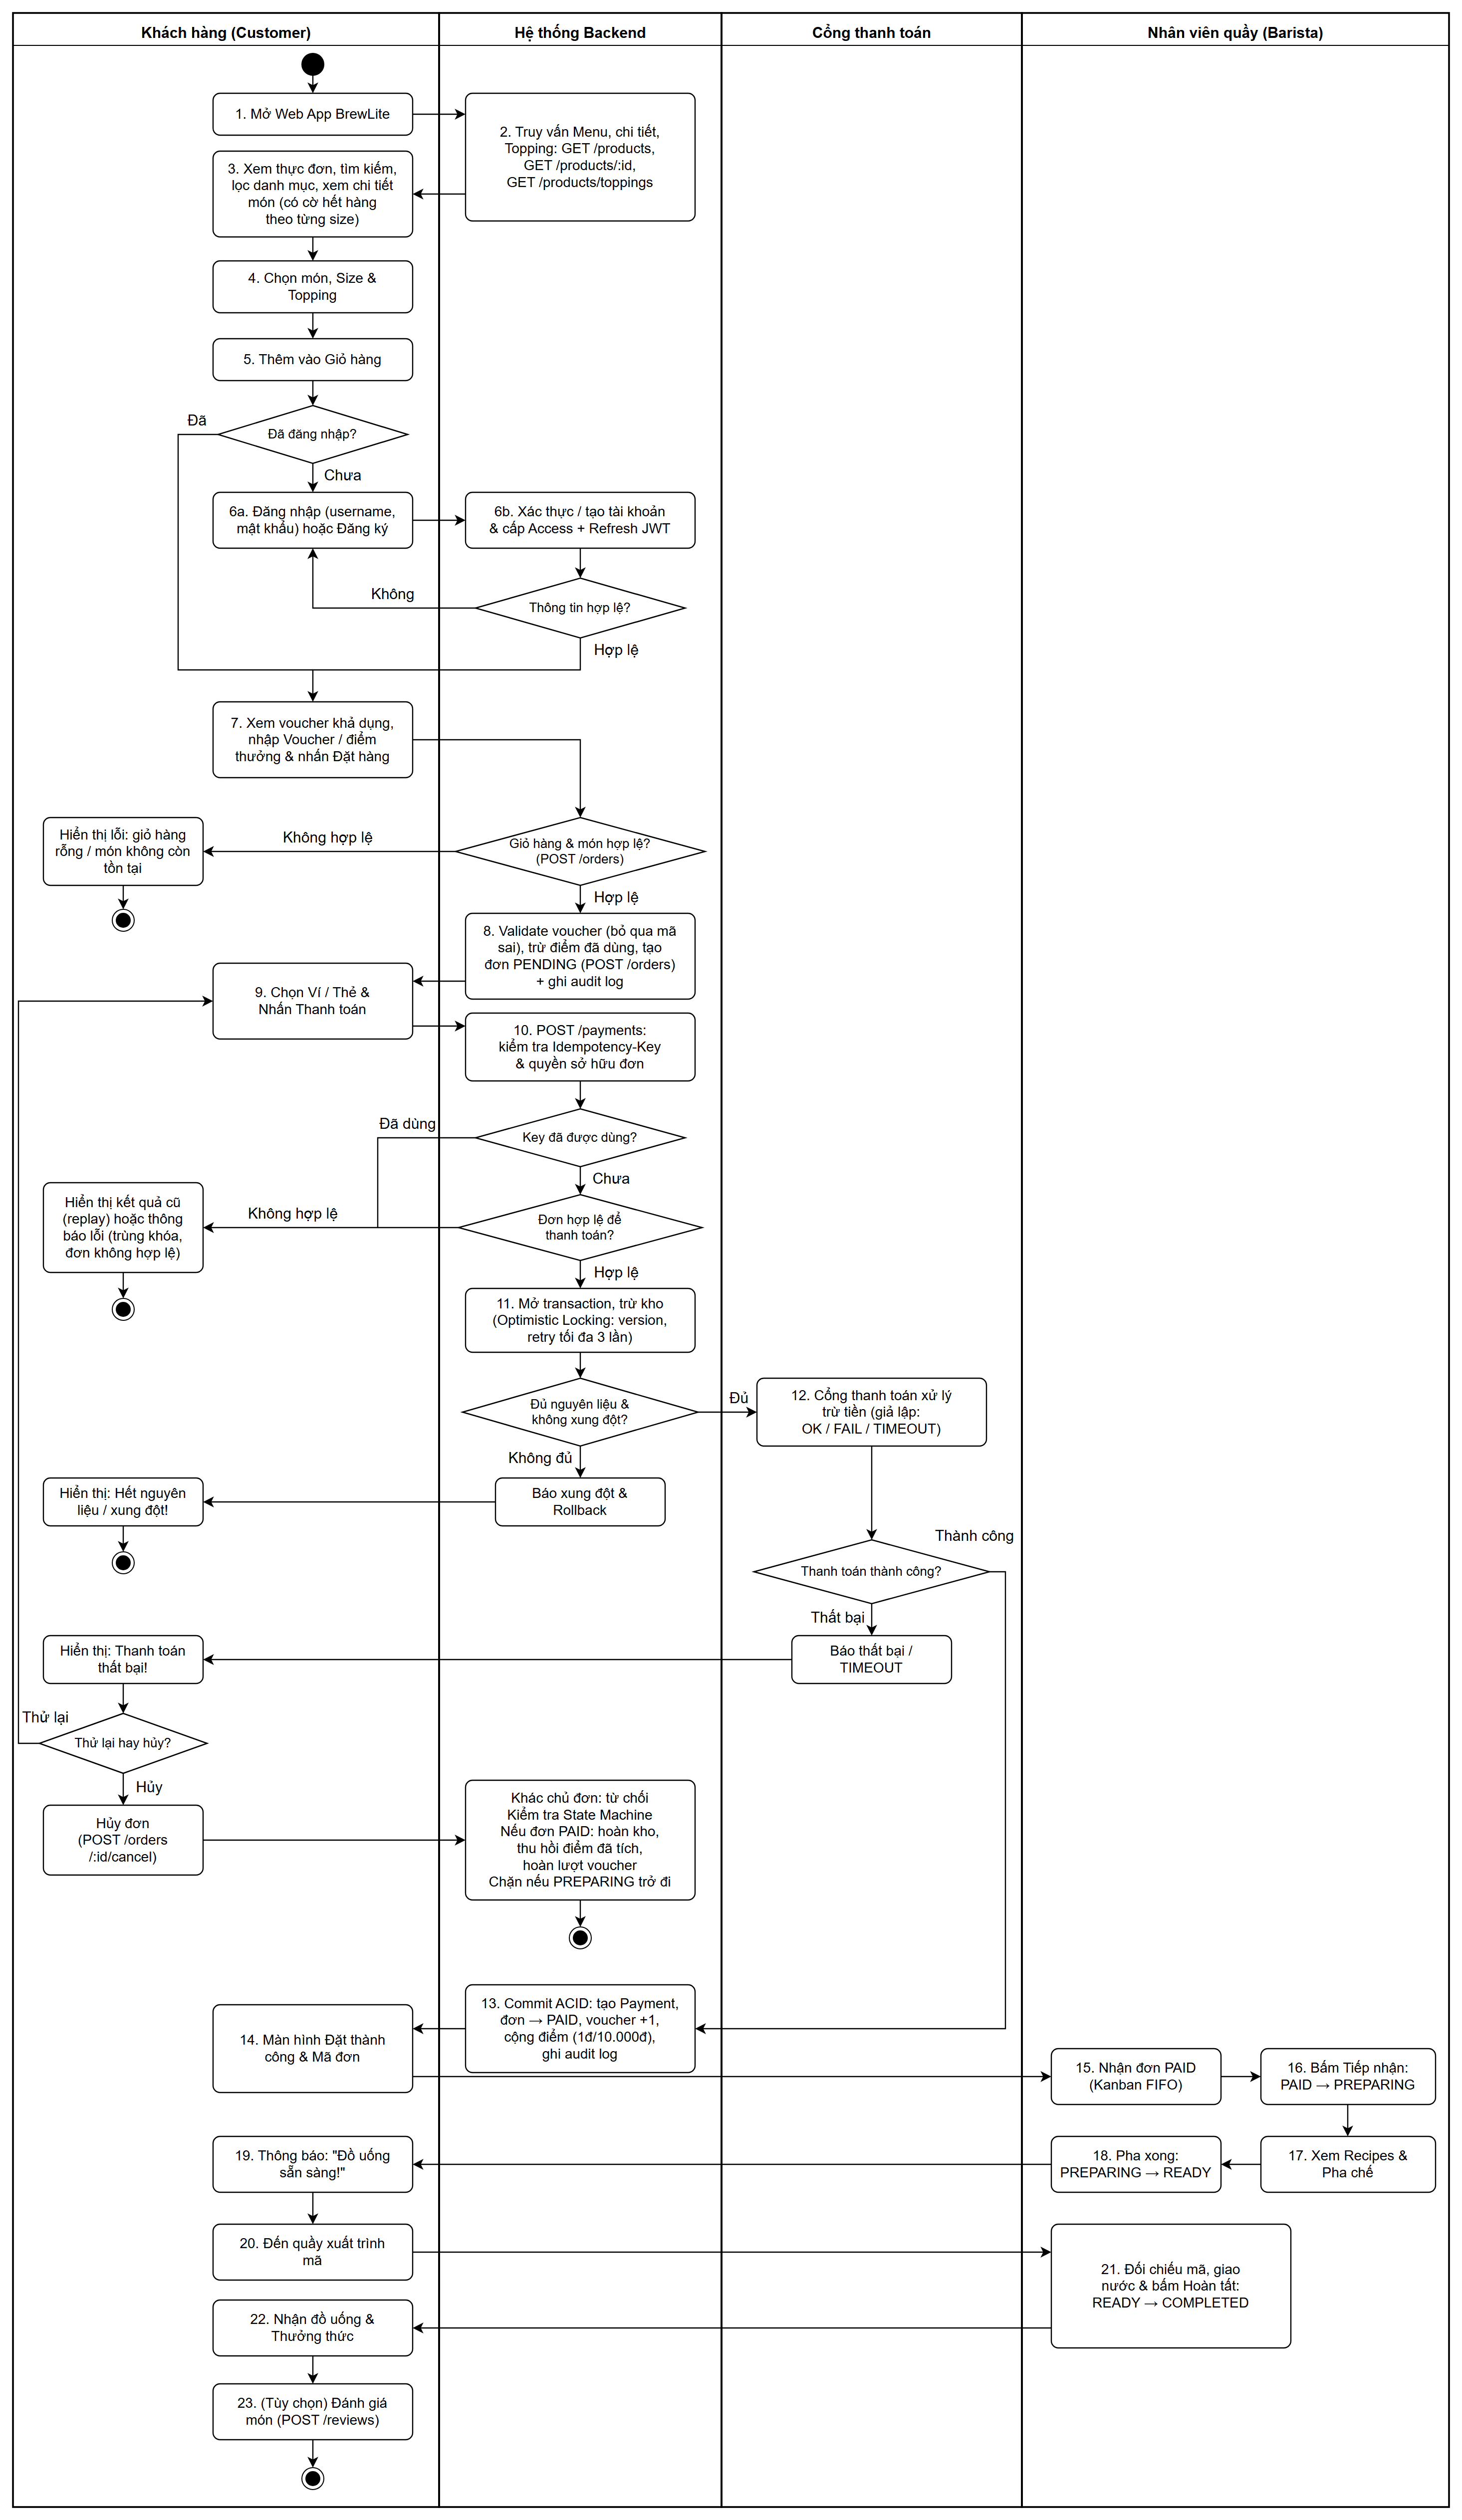
\includegraphics[width=1.08\textwidth,height=0.92\textheight,keepaspectratio]{img/activity-diagram.png}%
}
\caption{Sơ đồ hoạt động luồng đặt và thanh toán đơn hàng BrewLite}
\end{figure}

Sơ đồ sử dụng 4 swimlane --- Khách hàng (Customer), Hệ thống Backend, Cổng thanh toán và Nhân viên quầy (Barista) --- với điểm bắt đầu và điểm kết thúc rõ ràng. Luồng chính gồm 22 bước, được tóm tắt theo ba giai đoạn trong Bảng 2.1; các điểm rẽ nhánh xử lý trường hợp đặc biệt được liệt kê trong Bảng 2.2.

\begin{longtable}{>{\raggedright\arraybackslash}p{3.2cm}>{\raggedright\arraybackslash}p{2.2cm}>{\raggedright\arraybackslash}p{9.6cm}}
\caption{Các giai đoạn chính của luồng đặt và thanh toán}\\
\hline
\rowcolor{gray!20} \textbf{Giai đoạn} & \textbf{Bước} & \textbf{Nội dung} \\
\hline
\endfirsthead
\hline
\rowcolor{gray!20} \textbf{Giai đoạn} & \textbf{Bước} & \textbf{Nội dung} \\
\hline
\endhead
Xem menu và chuẩn bị đặt hàng & 1--6 & Khách hàng mở Web App, hệ thống truy vấn menu (GET /products); khách hàng xem thực đơn, chọn món kèm Size \& Topping và thêm vào giỏ hàng; nhánh chưa đăng nhập thực hiện xác thực và cấp JWT (6a, 6b) rồi hợp nhất vào luồng chính. \\
\hline
Đặt đơn và thanh toán & 7--14 & Khách hàng nhập voucher và đặt hàng, backend tạo đơn PENDING (POST /orders); khách hàng thanh toán, backend nhận POST /payments (Idempotency) và kiểm tra kho bằng Optimistic Locking (bước 11); khi thanh toán thành công, hệ thống thực hiện ACID Transaction chuyển đơn PENDING $\rightarrow$ PAID đồng thời trừ kho (bước 13) rồi hiển thị mã đơn (bước 14). \\
\hline
Pha chế và nhận món & 15--22 & Nhân viên quầy nhận đơn PAID trên bảng Kanban FIFO (bước 15), tiếp nhận (PAID $\rightarrow$ PREPARING), xem công thức và pha chế (bước 17), hoàn tất (PREPARING $\rightarrow$ READY); khách hàng nhận thông báo, đến quầy xuất trình mã và nhận đồ uống (bước 19--22). \\
\hline
\end{longtable}

\begin{longtable}{>{\raggedright\arraybackslash}p{3.4cm}>{\raggedright\arraybackslash}p{4.2cm}>{\raggedright\arraybackslash}p{7.4cm}}
\caption{Các điểm rẽ nhánh xử lý trường hợp đặc biệt}\\
\hline
\rowcolor{gray!20} \textbf{Điểm rẽ} & \textbf{Điều kiện} & \textbf{Xử lý} \\
\hline
\endfirsthead
\hline
\rowcolor{gray!20} \textbf{Điểm rẽ} & \textbf{Điều kiện} & \textbf{Xử lý} \\
\hline
\endhead
Đã đăng nhập? & Khách hàng chưa đăng nhập & Thực hiện 6a.~Nhập Email \& Mật khẩu và 6b.~Xác thực \& Cấp JWT, sau đó hợp nhất vào luồng chính. \\
\hline
Đủ nguyên liệu? & Tồn kho không đủ (bước 11) & Ném HTTP 409 và rollback; khách hàng nhận thông báo ``Hết nguyên liệu'', luồng kết thúc. \\
\hline
Thanh toán thành công? & Giao dịch thất bại (bước 12) & Thông báo thất bại cho khách hàng, luồng kết thúc; đơn hàng giữ trạng thái PENDING và có thể thanh toán lại. \\
\hline
\end{longtable}

Sơ đồ đáp ứng các yêu cầu của Task 2.1: có điểm bắt đầu/kết thúc, decision/merge cho các nhánh thành công và thất bại, swimlane cho cả bốn bên tham gia, và bao phủ đầy đủ ba trường hợp bắt buộc (hết hàng, chưa đăng nhập, thanh toán thất bại).

\section{Biểu đồ tuần tự (Sequence Diagram)}

Biểu đồ tuần tự mô tả chi tiết use-case trọng tâm ``Đặt và thanh toán đơn hàng'' (UC-12 + UC-13, tương ứng FR-06, FR-07, FR-09) ở mức gọi API (Hình 2.2).

\begin{figure}[p]
\centering
\makebox[\textwidth][c]{%
  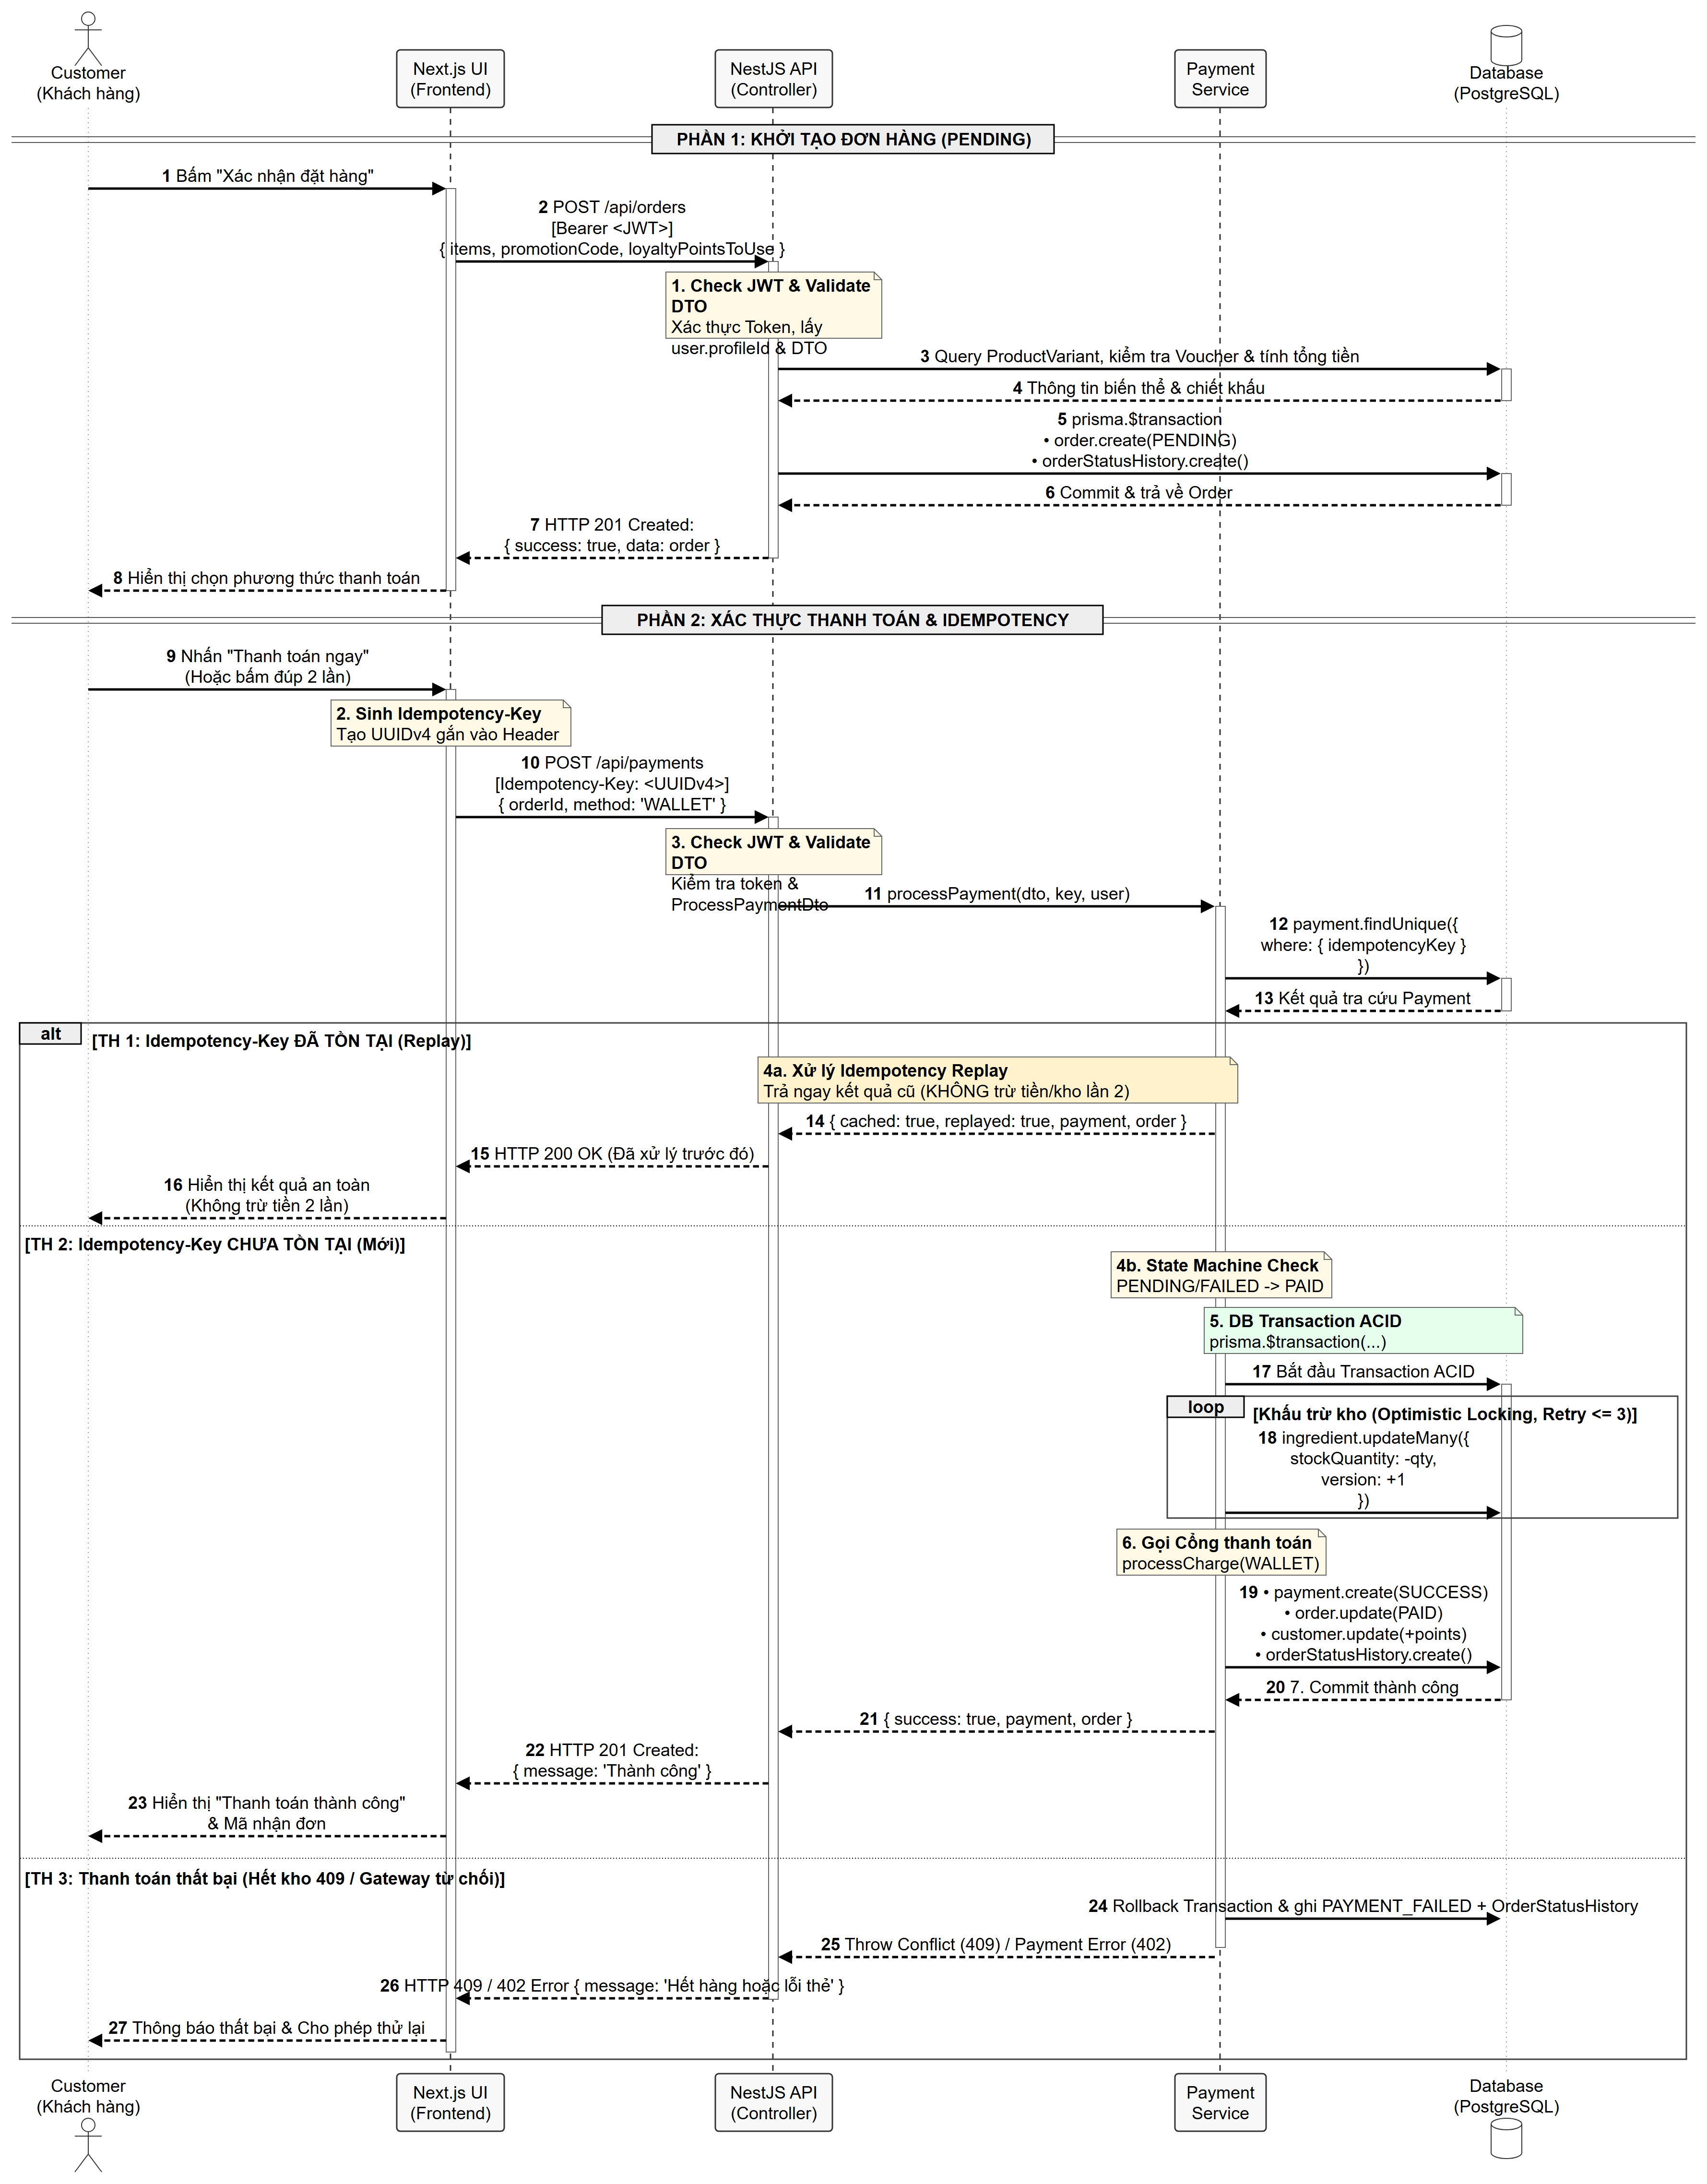
\includegraphics[width=1.08\textwidth,height=0.92\textheight,keepaspectratio]{img/Sequence_Diagram.png}%
}
\caption{Biểu đồ tuần tự Đặt và thanh toán đơn hàng}
\end{figure}

Sơ đồ gồm 5 lifeline --- Khách hàng (actor), Next.js UI (Frontend App), NestJS API (Controller \& Guard), Payment Service (Business Logic) và Database --- được chia làm hai phân đoạn chính (Bảng 2.3). Các cơ chế kỹ thuật then chốt trong luồng được tóm tắt trong Bảng 2.4.

\begin{longtable}{>{\raggedright\arraybackslash}p{4.0cm}>{\raggedright\arraybackslash}p{11.2cm}}
\caption{Hai phân đoạn chính của biểu đồ tuần tự}\\
\hline
\rowcolor{gray!20} \textbf{Phân đoạn} & \textbf{Luồng chính} \\
\hline
\endfirsthead
\hline
\rowcolor{gray!20} \textbf{Phân đoạn} & \textbf{Luồng chính} \\
\hline
\endhead
1. Khởi tạo đơn hàng (PENDING) & Khách hàng bấm ``Xác nhận đặt hàng'' trên UI; UI gọi POST /api/orders (Header: Authorization: Bearer \texttt{<JWT>}, Body: \texttt{\{ items, promotionCode \}}) tới NestJS API. API kiểm tra JWT (JwtAuthGuard giải mã Bearer Token, lấy user.profileId), truy vấn ProductVariant, kiểm tra Voucher và tính tổng tiền, rồi tạo đơn trong \textit{prisma.\$transaction} (tx.order.create với status PENDING và tx.orderStatusHistory.create) và trả về HTTP 201 Created với đơn hàng PENDING. \\
\hline
2. Xác thực thanh toán \& chống click đúp & UI sinh Idempotency-Key (UUIDv4) gắn vào Header rồi gọi POST /api/payments (Body: \texttt{\{ orderId, method: 'WALLET' \}}). API kiểm tra lại JWT và chuyển sang Payment Service (processPayment); Payment Service tra cứu Payment theo Idempotency-Key. Khối \textit{alt} có hai trường hợp: key đã tồn tại thì trả ngay kết quả cũ (HTTP 200 OK, cached: true, replayed: true), không trừ tiền lần hai; key chưa tồn tại thì kiểm tra máy trạng thái (assertTransition, chỉ PENDING / PAYMENT\_FAILED sang PAID) rồi thực hiện Database Transaction ACID qua \textit{prisma.\$transaction}: trừ kho bằng Optimistic Locking (khối \textit{loop}, retry tối đa 3 lần), gọi cổng thanh toán mô phỏng (mockGateway.processCharge), tạo giao dịch, chuyển đơn sang PAID, cộng điểm Loyalty và ghi OrderStatusHistory; kết quả trả về UI (HTTP 201 Created) và hiển thị cho khách hàng. \\
\hline
\end{longtable}

\begin{longtable}{>{\raggedright\arraybackslash}p{3.8cm}>{\raggedright\arraybackslash}p{11.4cm}}
\caption{Các cơ chế kỹ thuật trong luồng thanh toán}\\
\hline
\rowcolor{gray!20} \textbf{Cơ chế} & \textbf{Mô tả} \\
\hline
\endfirsthead
\hline
\rowcolor{gray!20} \textbf{Cơ chế} & \textbf{Mô tả} \\
\hline
\endhead
Xác thực JWT & JwtAuthGuard kiểm tra Bearer Token ở cả hai API, xác thực tính hợp lệ và lấy định danh người dùng. \\
\hline
Idempotency-Key & UI tự động sinh UUIDv4 duy nhất cho mỗi lần thanh toán, gắn vào Header của POST /payments. \\
\hline
Idempotency Replay & Phát hiện Idempotency-Key đã tồn tại thì trả ngay kết quả cũ (HTTP 200 OK, cached: true, replayed: true), KHÔNG gọi trừ tiền và KHÔNG trừ kho lần hai. \\
\hline
Kiểm tra máy trạng thái & \textit{assertTransition(order.status, 'PAID')}: chỉ cho phép chuyển từ PENDING hoặc PAYMENT\_FAILED sang PAID. \\
\hline
Database Transaction & Mọi thao tác ghi (tạo giao dịch, trừ kho, chuyển trạng thái, cộng điểm Loyalty, ghi OrderStatusHistory) thực hiện trong ACID Transaction qua \textit{prisma.\$transaction}. \\
\hline
Khấu trừ kho (Optimistic Locking) & Khối \textit{loop} trừ kho nguyên liệu bằng tx.ingredient.updateMany với điều kiện version và stockQuantity, retry tối đa 3 lần. \\
\hline
Cổng thanh toán mô phỏng & Gọi \textit{mockGateway.processCharge(\{ amount, method: 'WALLET' \})} để xử lý trừ tiền trong phạm vi MVP. \\
\hline
\end{longtable}

\section{Sơ đồ lớp (Class Diagram)}

Sơ đồ lớp mô hình hóa cấu trúc dữ liệu mức domain của BrewLite gồm 16 lớp và 1 enumeration (Hình 2.3).

\begin{figure}[p]
\centering
\makebox[\textwidth][c]{%
  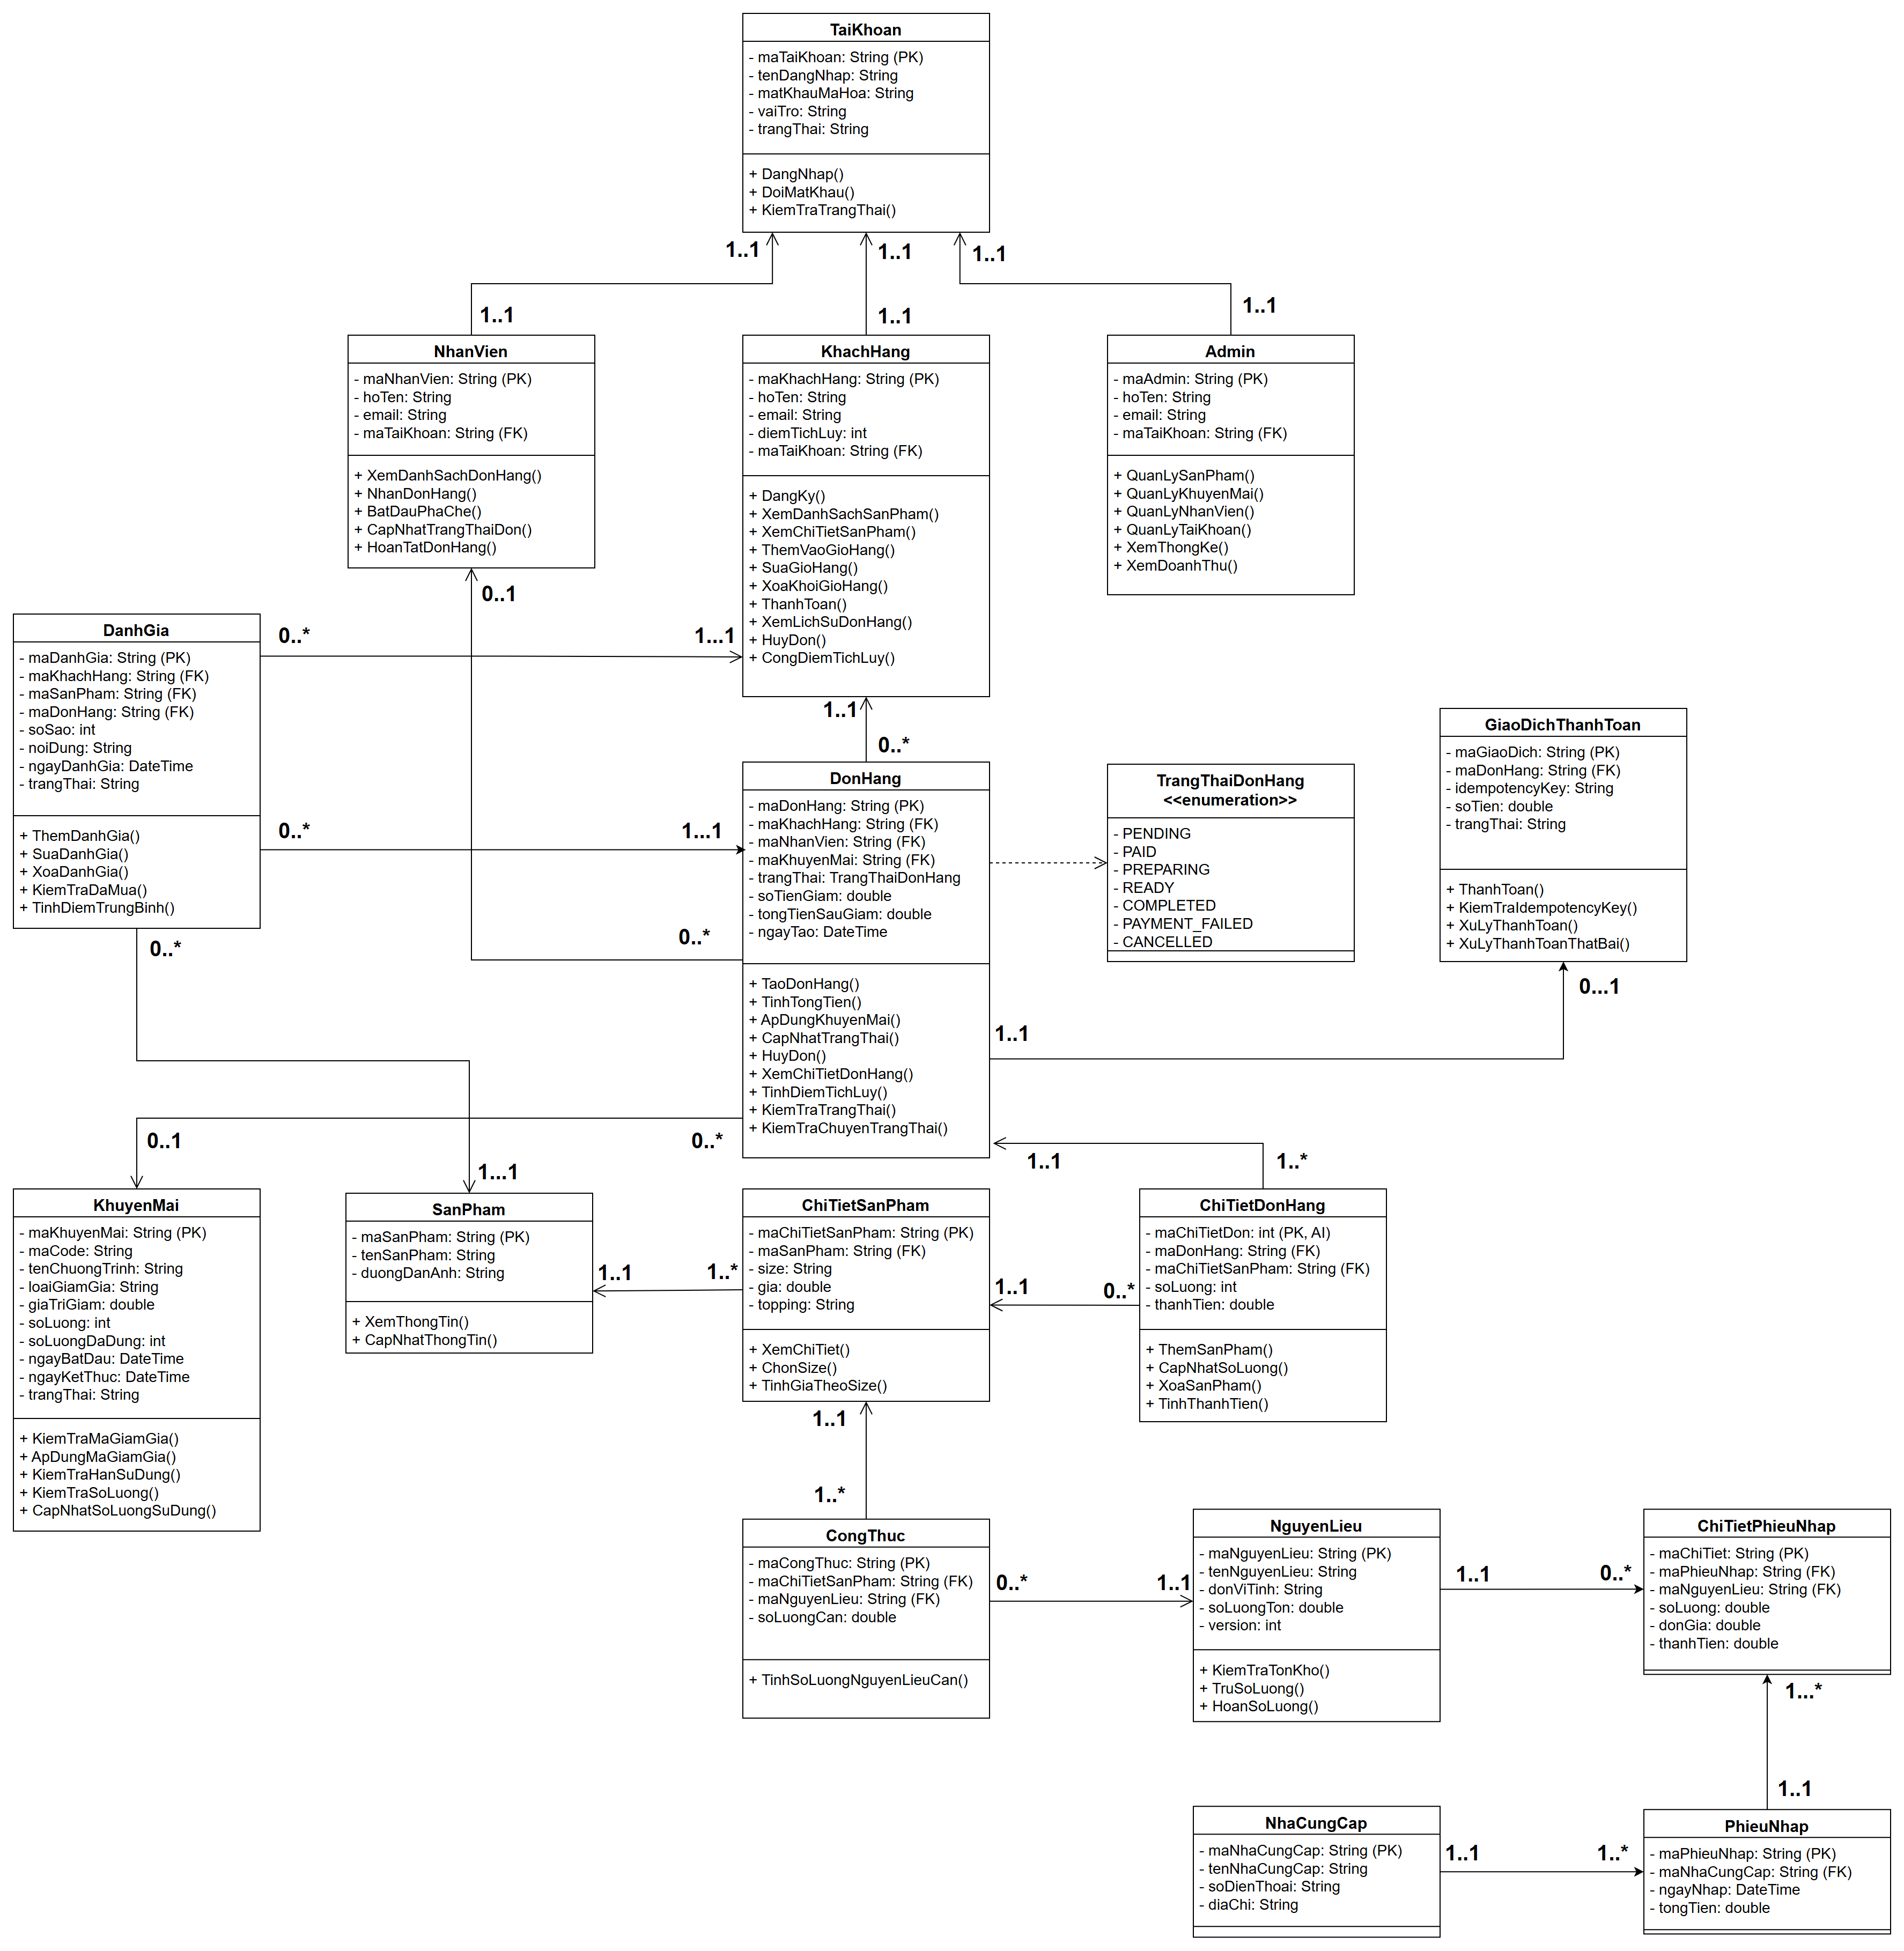
\includegraphics[width=1.08\textwidth,height=0.92\textheight,keepaspectratio]{img/class-diagram.png}%
}
\caption{Sơ đồ lớp hệ thống BrewLite}
\end{figure}

Các lớp được nhóm theo nghiệp vụ như trong Bảng 2.5. \textit{TrangThaiDonHang} là enumeration gồm 7 giá trị (PENDING, PAID, PREPARING, READY, COMPLETED, PAYMENT\_FAILED, CANCELLED), dùng làm kiểu dữ liệu cho thuộc tính trangThai của DonHang.

\begin{longtable}{>{\raggedright\arraybackslash}p{3.8cm}>{\raggedright\arraybackslash}p{11.4cm}}
\caption{Các nhóm lớp trong sơ đồ lớp}\\
\hline
\rowcolor{gray!20} \textbf{Nhóm} & \textbf{Các lớp} \\
\hline
\endfirsthead
\hline
\rowcolor{gray!20} \textbf{Nhóm} & \textbf{Các lớp} \\
\hline
\endhead
Người dùng và phân quyền & \textit{TaiKhoan} (tài khoản dùng chung: DangNhap(), DoiMatKhau(), KiemTraTrangThai()); \textit{KhachHang} (DangKy(), XemDanhSachSanPham(), XemChiTietSanPham(), ThemVaoGioHang(), SuaGioHang(), XoaKhoiGioHang(), ThanhToan(), XemLichSuDonHang(), HuyDon(), CongDiemTichLuy()); \textit{NhanVien} (nghiệp vụ quầy: XemDanhSachDonHang(), NhanDonHang(), BatDauPhaChe(), CapNhatTrangThaiDon(), HoanTatDonHang()); \textit{Admin} (QuanLySanPham(), QuanLyKhuyenMai(), QuanLyNhanVien(), QuanLyTaiKhoan(), XemThongKe(), XemDoanhThu()). \\
\hline
Bán hàng & \textit{SanPham} (XemThongTin(), CapNhatThongTin()); \textit{ChiTietSanPham} (size, giá, topping; XemChiTiet(), ChonSize(), TinhGiaTheoSize()); \textit{DonHang} (trạng thái kiểu TrangThaiDonHang; TaoDonHang(), TinhTongTien(), ApDungKhuyenMai(), CapNhatTrangThai(), HuyDon(), XemChiTietDonHang(), TinhDiemTichLuy(), KiemTraTrangThai(), KiemTraChuyenTrangThai()); \textit{ChiTietDonHang} (ThemSanPham(), CapNhatSoLuong(), XoaSanPham(), TinhThanhTien()); \textit{KhuyenMai} (KiemTraMaGiamGia(), ApDungMaGiamGia(), KiemTraHanSuDung(), KiemTraSoLuong(), CapNhatSoLuongSuDung()). \\
\hline
Thanh toán & \textit{GiaoDichThanhToan} (maGiaoDich, maDonHang, idempotencyKey, soTien, trangThai; ThanhToan(), KiemTraIdempotencyKey(), XuLyThanhToan(), XuLyThanhToanThatBai()), quan hệ 0..1 với DonHang (một DonHang có tối đa một giao dịch). \\
\hline
Kho và nguyên liệu & \textit{NguyenLieu} (\textit{version: int} phục vụ Optimistic Locking; KiemTraTonKho(), TruSoLuong(), HoanSoLuong()); \textit{CongThuc} (nối ChiTietSanPham với NguyenLieu; TinhSoLuongNguyenLieuCan()); \textit{NhaCungCap}, \textit{PhieuNhap}, \textit{ChiTietPhieuNhap} (nghiệp vụ nhập hàng). \\
\hline
Đánh giá & \textit{DanhGia} (soSao, noiDung; ThemDanhGia(), SuaDanhGia(), XoaDanhGia(), KiemTraDaMua(), TinhDiemTrungBinh()), gắn với KhachHang, SanPham và DonHang. \\
\hline
\end{longtable}

Các quan hệ chính (multiplicity ghi trên sơ đồ): một KhachHang có nhiều DonHang (0..*); một DonHang gồm nhiều ChiTietDonHang (1..*); ChiTietDonHang tham chiếu đúng một ChiTietSanPham (1..1); DonHang áp dụng tối đa một KhuyenMai (0..1) và do tối đa một NhanVien phụ trách (0..1); KhachHang, NhanVien và Admin mỗi người sở hữu một TaiKhoan. Đối chiếu với Task 2.3 được tóm tắt trong Bảng 2.6.

\begin{longtable}{>{\raggedright\arraybackslash}p{4.5cm}>{\raggedright\arraybackslash}p{10.7cm}}
\caption{Đối chiếu yêu cầu Task 2.3 với sơ đồ lớp}\\
\hline
\rowcolor{gray!20} \textbf{Yêu cầu} & \textbf{Lớp tương ứng} \\
\hline
\endfirsthead
\hline
\rowcolor{gray!20} \textbf{Yêu cầu} & \textbf{Lớp tương ứng} \\
\hline
\endhead
User & TaiKhoan, KhachHang, NhanVien, Admin \\
\hline
Product & SanPham, ChiTietSanPham \\
\hline
Order & DonHang \\
\hline
OrderItem & ChiTietDonHang \\
\hline
Payment & GiaoDichThanhToan \\
\hline
Promotion & KhuyenMai \\
\hline
LoyaltyTransaction & Thể hiện qua thuộc tính diemTichLuy và các phương thức CongDiemTichLuy()/TinhDiemTichLuy() (không tách thành lớp riêng) \\
\hline
\end{longtable}

\chapter{THIẾT KẾ KIẾN TRÚC HỆ THỐNG}

Chương này trình bày thiết kế kiến trúc hệ thống BrewLite theo Task 3 của Assignment 2: phương pháp kiến trúc và sơ đồ triển khai trên môi trường production thực tế.

\section{Phương pháp kiến trúc}

\subsection{Kiến trúc tổng thể hệ thống}

Hệ thống BrewLite được xây dựng theo kiến trúc phân lớp (layered architecture) gồm ba tầng chính. Tầng trình diễn (Presentation) là ứng dụng web Next.js 14 (App Router), hoạt động như Progressive Web App trên trình duyệt của khách hàng và nhân viên quầy. Tầng ứng dụng (Application) là backend NestJS 10 được tổ chức theo module, tiếp nhận REST API qua HTTPS, thực thi nghiệp vụ (máy trạng thái đơn hàng, idempotency thanh toán, optimistic locking tồn kho) và truy xuất dữ liệu qua Prisma ORM. Tầng dữ liệu (Data) là PostgreSQL 16, quản lý schema bằng migration.

Các tầng giao tiếp qua giao thức chuẩn mở: frontend gọi REST API tới backend; backend kết nối PostgreSQL qua TCP/IP; tích hợp cổng thanh toán bên thứ ba qua REST/Webhook. Mọi secret và cấu hình môi trường được quản lý tách biệt, không đưa vào mã nguồn. Các quyết định kiến trúc quan trọng (lựa chọn monorepo, PostgreSQL + Prisma, cổng thanh toán mô phỏng ở MVP) được ghi nhận dưới dạng ADR trong docs/architecture/adr.

\subsection{Danh sách các module}

Backend được tổ chức thành các module NestJS theo nghiệp vụ, liệt kê trong Bảng 3.1.

\begin{longtable}{>{\raggedright\arraybackslash}p{3.8cm}>{\raggedright\arraybackslash}p{11.4cm}}
\caption{Các module chính của backend}\\
\hline
\rowcolor{gray!20} \textbf{Module} & \textbf{Trách nhiệm} \\
\hline
\endfirsthead
\hline
\rowcolor{gray!20} \textbf{Module} & \textbf{Trách nhiệm} \\
\hline
\endhead
AuthModule & Đăng ký, đăng nhập, làm mới token, đổi mật khẩu và phân quyền theo vai trò (Customer, Staff, Admin). \\
\hline
ProductsModule & Quản lý thực đơn: danh sách món, chi tiết size/topping, kiểm tra cờ hết nguyên liệu (\texttt{GET /products}, \texttt{/products/:id}, \texttt{/products/toppings}). \\
\hline
OrdersModule & Khởi tạo đơn PENDING, máy trạng thái đơn hàng (\texttt{assertTransition}), theo dõi lịch sử và hủy đơn hoàn kho/điểm/voucher. \\
\hline
PaymentModule & Xử lý thanh toán idempotent (\texttt{idempotency-key}), tích hợp cổng thanh toán mô phỏng, trừ kho bằng Optimistic Locking (cột \texttt{version}), cộng điểm Loyalty và đồng bộ MBBank VietQR. \\
\hline
PromotionsModule & Tra cứu voucher khả dụng (\texttt{GET /promotions/available}) và kiểm tra, tính toán giảm giá (\texttt{POST /promotions/validate}). \\
\hline
StaffModule & API cho nhân viên pha chế: bảng Kanban FIFO (\texttt{GET /staff/orders}), công thức pha chế (\texttt{/recipes}), cập nhật trạng thái (\texttt{/accept}, \texttt{/ready}, \texttt{/complete}). \\
\hline
ReviewsModule & Đánh giá món thuộc đơn đã \texttt{COMPLETED}, chỉnh sửa và xóa đánh giá chính chủ. \\
\hline
AdminModule & Thống kê doanh thu, quản lý kho nguyên liệu, nhà cung cấp, phiếu nhập kho, sản phẩm/công thức, khuyến mãi, kiểm duyệt đánh giá và tài khoản. \\
\hline
\end{longtable}

\subsection{Các bản ghi quyết định kiến trúc (Architecture Decision Records -- ADR)}

Theo đúng quy định của Task 3.1, các quyết định kiến trúc quan trọng của dự án được lưu thành 5 bản ghi ADR ngắn trong thư mục \texttt{docs/architecture/adr/} (Bảng 3.2).

\begin{longtable}{>{\centering\arraybackslash}p{1.8cm}>{\raggedright\arraybackslash}p{3.8cm}>{\raggedright\arraybackslash}p{9.6cm}}
\caption{Danh mục các bản ghi quyết định kiến trúc (ADR)}\\
\hline
\rowcolor{gray!20} \textbf{Mã ADR} & \textbf{Quyết định} & \textbf{Lý do lựa chọn và đánh đổi (Trade-off)} \\
\hline
\endfirsthead
\hline
\rowcolor{gray!20} \textbf{Mã ADR} & \textbf{Quyết định} & \textbf{Lý do lựa chọn và đánh đổi (Trade-off)} \\
\hline
\endhead
ADR-001 & Cấu trúc Monorepo & Quản lý cả Frontend (\texttt{frontend/}) và Backend (\texttt{backend/}) trong cùng một repository giúp đồng bộ tài liệu, Docker Compose và quy trình CI/CD. \\
\hline
ADR-002 & Backend NestJS Modular & Tổ chức NestJS theo từng domain module (\texttt{auth}, \texttt{products}, \texttt{orders}, \texttt{payment}, \texttt{staff}, \texttt{admin}...) giúp tách biệt trách nhiệm rõ ràng và dễ viết unit test với Jest. \\
\hline
ADR-003 & Next.js Mobile-First PWA & Sử dụng Next.js 14 App Router, Tailwind CSS và cấu hình PWA (\texttt{manifest.json}) để tối ưu trải nghiệm đặt món trên di động lẫn desktop. \\
\hline
ADR-004 & PostgreSQL \& Prisma ORM & Dùng PostgreSQL 16 kết hợp Prisma ORM nhằm bảo đảm an toàn kiểu dữ liệu (type-safety), quản lý migration và hỗ trợ transaction ACID chặt chẽ. \\
\hline
ADR-005 & Idempotency \& State Machine & Kết hợp \texttt{idempotency-key} trên thanh toán, máy trạng thái đơn hàng (\texttt{assertTransition}) và Optimistic Locking (\texttt{version}) để chống trừ tiền trùng và chống bán âm kho. \\
\hline
\end{longtable}

\subsection{Các tiêu chí phi chức năng}

Kiến trúc trên được thiết kế nhằm đáp ứng các tiêu chí phi chức năng sau (trích từ NFR-01 đến NFR-06):

\begin{enumerate}[leftmargin=*]
\item \textbf{Hiệu năng:} thời gian phản hồi API cốt lõi dưới 500ms với dữ liệu mẫu; hỗ trợ phân trang danh sách sản phẩm.
\item \textbf{Nền tảng và giao diện:} Responsive Web + PWA, giao diện tiếng Việt; màn hình quầy tối ưu thao tác nhanh.
\item \textbf{Đồng thời và toàn vẹn dữ liệu:} Optimistic Locking chống bán âm; mọi thao tác ghi quan trọng thực hiện trong \texttt{prisma.\$transaction}.
\item \textbf{Bảo mật:} mật khẩu băm bcrypt (10 rounds), JWT + phân quyền RBAC (\texttt{CUSTOMER}, \texttt{STAFF}, \texttt{ADMIN}), HTTPS ở môi trường production, validate đầu vào qua \texttt{class-validator}.
\item \textbf{Triển khai và vận hành:} đóng gói Docker/Docker Compose; CI/CD tự động kiểm tra mã nguồn; health check endpoint (\texttt{/health}, \texttt{/api/health}) và hướng dẫn rollback.
\end{enumerate}

\section{Sơ đồ triển khai hệ thống}

Sơ đồ triển khai (Deployment Diagram) mô tả cách các thành phần của BrewLite được phân bố trên môi trường production thực tế (Hình 3.1).

\begin{figure}[!htbp]
\centering
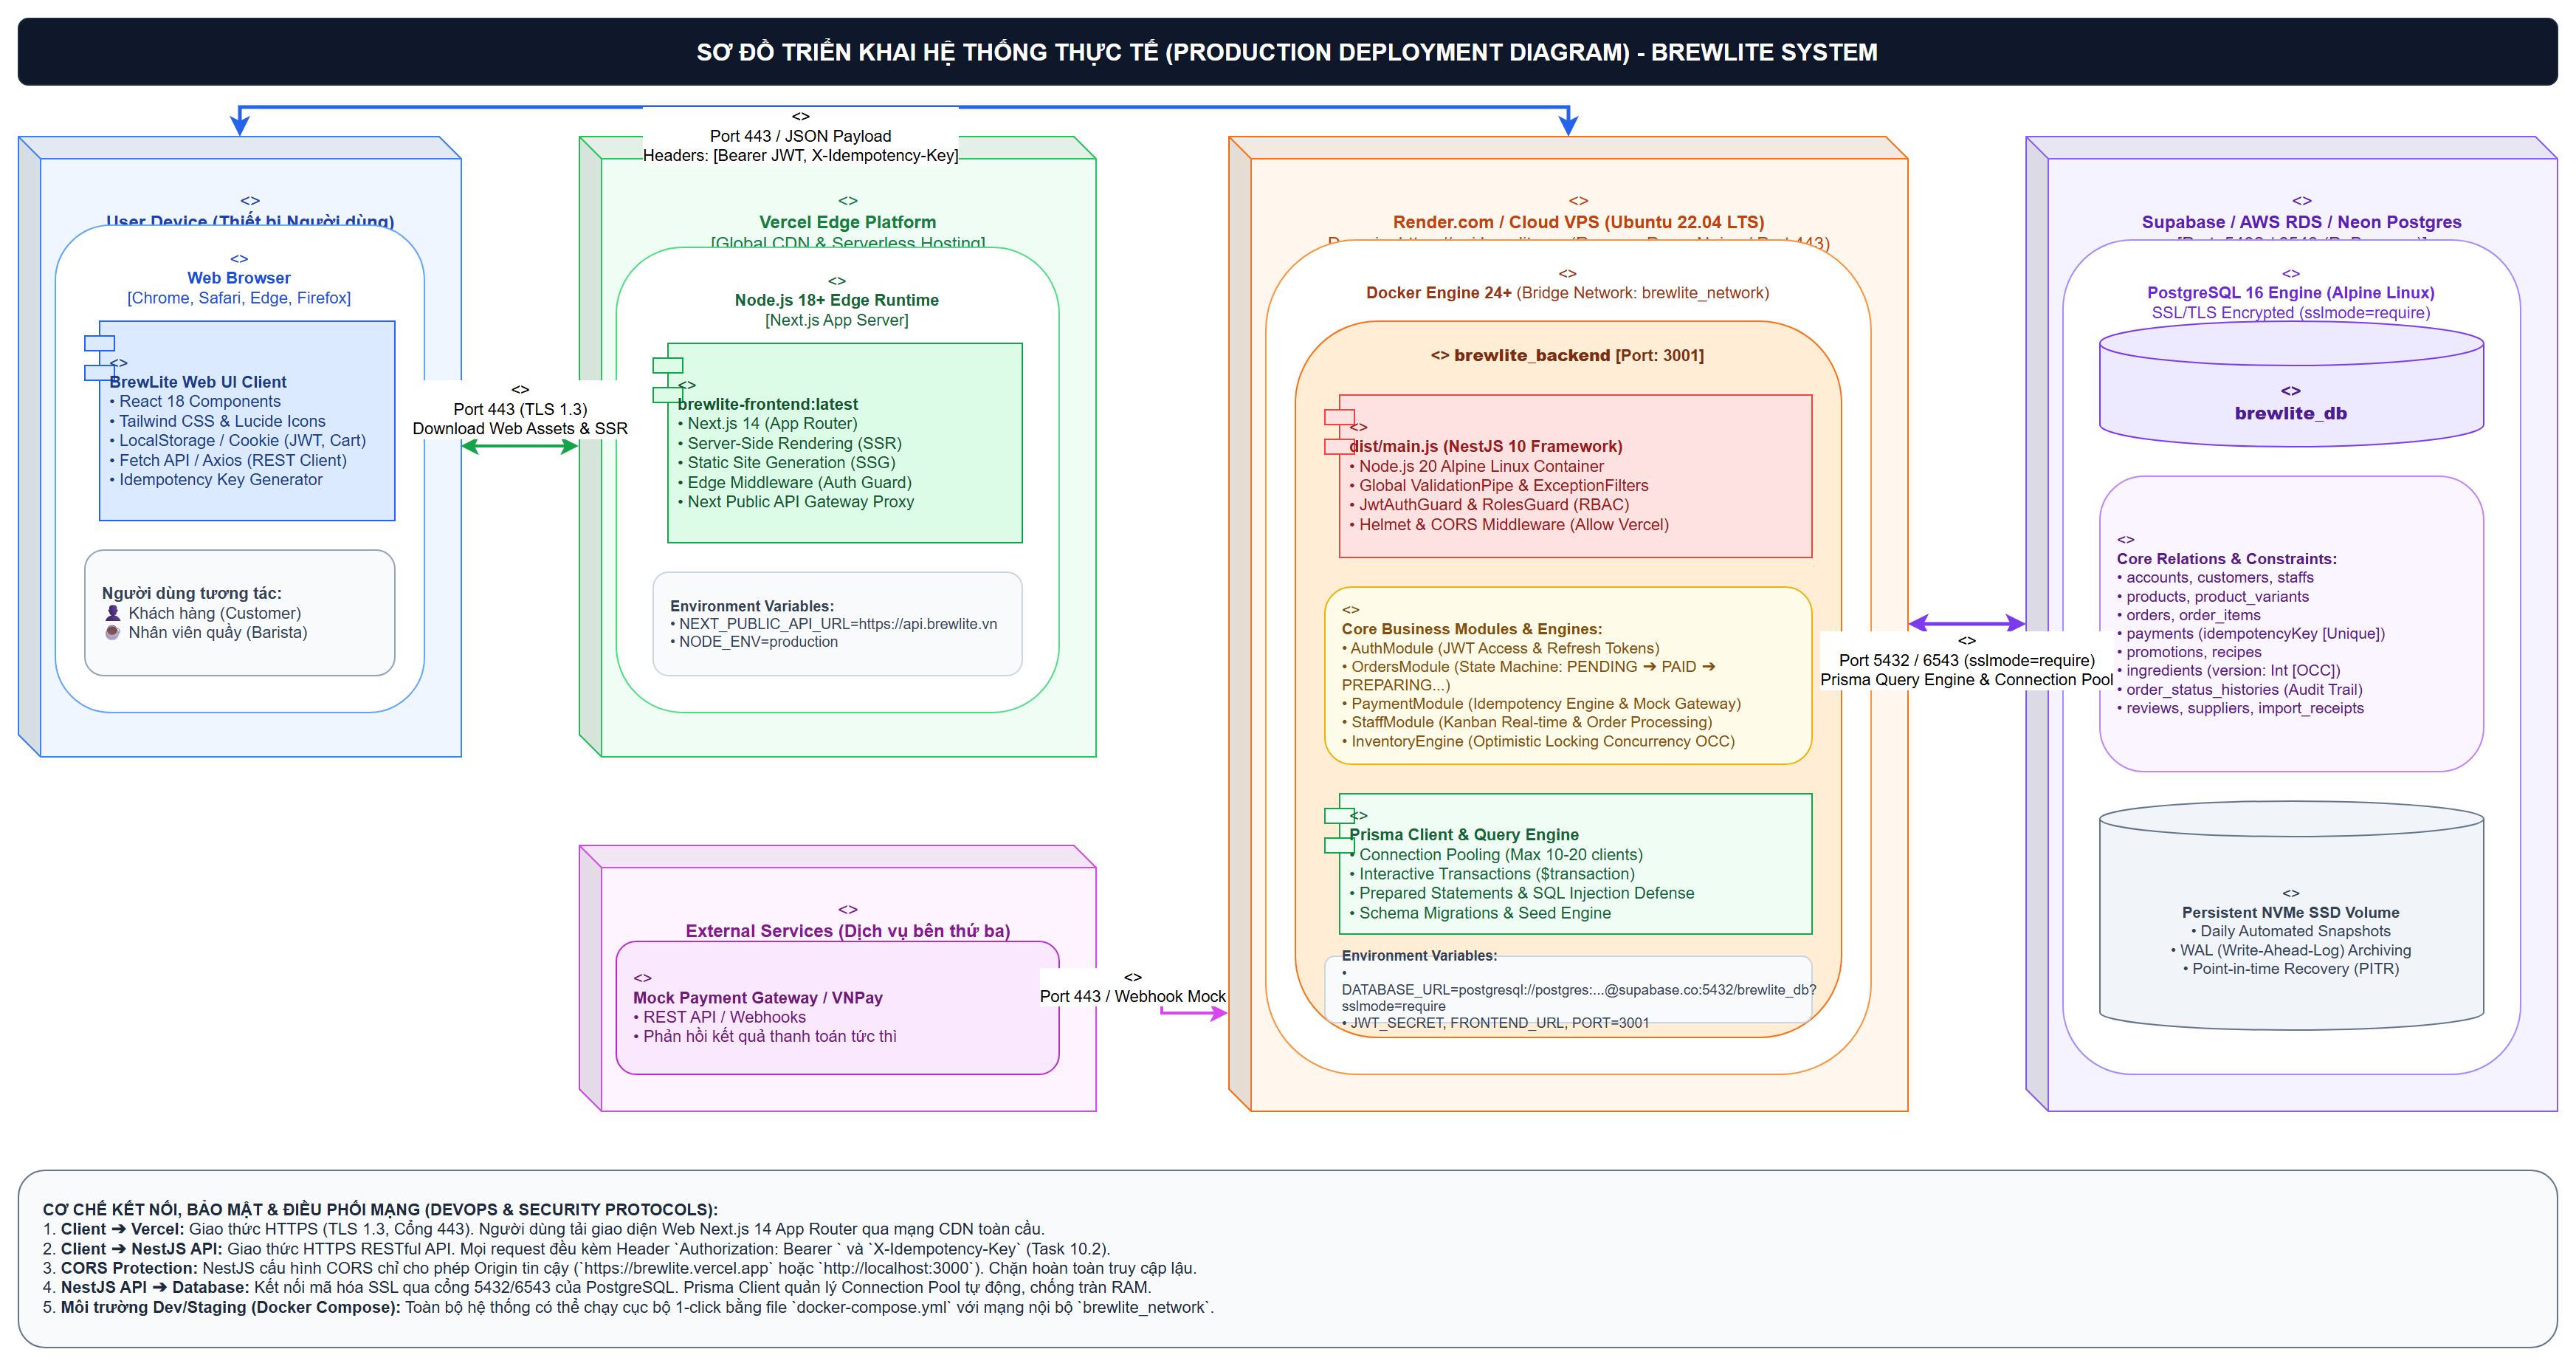
\includegraphics[width=\textwidth]{img/deployment-brewlite.png}
\caption{Sơ đồ triển khai hệ thống BrewLite}
\end{figure}

Các thành phần chính được mô tả trong Bảng 3.3.

\begin{longtable}{>{\raggedright\arraybackslash}p{3.8cm}>{\raggedright\arraybackslash}p{11.4cm}}
\caption{Các thành phần triển khai hệ thống}\\
\hline
\rowcolor{gray!20} \textbf{Thành phần} & \textbf{Mô tả} \\
\hline
\endfirsthead
\hline
\rowcolor{gray!20} \textbf{Thành phần} & \textbf{Mô tả} \\
\hline
\endhead
Thiết bị người dùng & Laptop/PC/Mobile chạy trình duyệt web; BrewLite Web UI Client (React 18, Tailwind) gắn Idempotency-Key vào mỗi yêu cầu thanh toán, gọi REST API qua HTTPS (port 443). \\
\hline
Vercel Serverless Edge Platform & Nền tảng \guillemotleft{}cloud/PaaS\guillemotright{} triển khai frontend \textit{brewlite-frontend} (Next.js 14, App Router); gọi API sang backend. \\
\hline
Application Server & Render.com / Cloud VPS (Ubuntu 22.04) chạy Docker Engine 24+ (mạng brewlite\_network); container \textit{brewlite\_backend} (port 3001) gồm NestJS 10 + Prisma ORM và bốn core engine: AuthModule, Orders State Machine, Payment Idempotency, Inventory Optimistic Locking (OCC). \\
\hline
Database Server & Supabase / AWS RDS Postgres chạy PostgreSQL 16 (port 5432/6543); cơ sở dữ liệu \textit{brewlite\_db} (17 bảng), giao tiếp với backend qua TCP/IP port 5432. \\
\hline
Dịch vụ bên thứ ba & Mock Payment Gateway / VNPay (\guillemotleft{}thirdPartyCloud\guillemotright{}), tích hợp với backend qua REST/Webhook để xử lý và nhận kết quả thanh toán. \\
\hline
\end{longtable}

Sơ đồ phản ánh đúng nền tảng production thực tế mà nhóm sử dụng, đáp ứng yêu cầu Task 3.2 của Assignment 2.

\chapter{TRIỂN KHAI SPRINT 1 (TASK 4)}

Sprint 1 thực hiện mục tiêu tạo nền tảng kỹ thuật chuẩn hóa cho kho mã nguồn, quản lý tài liệu theo phiên bản, xây dựng MVP đầu tiên cho luồng xem thực đơn và thiết lập pipeline Continuous Integration (CI).

\section{Thiết lập Repository và Quản lý tài liệu (Task 4.1 \& 4.2)}

\subsection{Cấu trúc kho mã nguồn Monorepo}
Kho mã nguồn được lưu trữ công khai trên GitHub tại \url{https://github.com/hanhdevsgu/BrewLite-Assignment2}, tổ chức theo cấu trúc:
\begin{itemize}[leftmargin=*]
\item \texttt{frontend/}: Ứng dụng web Next.js 14 App Router (TypeScript, Tailwind CSS, Zustand, PWA).
\item \texttt{backend/}: Dịch vụ REST API NestJS 10 (TypeScript, Prisma ORM, PostgreSQL 16).
\item \texttt{docs/}: Toàn bộ tài liệu yêu cầu (\texttt{requirements/}), sơ đồ UML nguồn \& xuất ảnh (\texttt{diagrams/}), thiết kế kiến trúc \& 5 ADR (\texttt{architecture/}), ma trận truy vết (\texttt{traceability-matrix.md}), hướng dẫn triển khai (\texttt{deployment.md}), rollback (\texttt{rollback-guide.md}) và Sprint Retrospective (\texttt{sprints/}).
\item \texttt{tests/}: Kịch bản kiểm thử đầu-cuối (\texttt{tests/e2e/order-checkout.e2e-spec.ts}).
\item \texttt{.github/workflows/}: Cấu hình GitHub Actions cho CI (\texttt{ci.yml}) và CD (\texttt{cd.yml}).
\item \texttt{docker-compose.yml}, \texttt{.env.example}, \texttt{README.md}: Đóng gói chạy đồng bộ 3 dịch vụ và hướng dẫn cài đặt chi tiết.
\end{itemize}

\subsection{Chiến lược phân nhánh, Quy ước Commit và Definition of Done}
\begin{itemize}[leftmargin=*]
\item \textbf{Chiến lược nhánh}: Nhánh \texttt{main} (sản phẩm ổn định), \texttt{develop} (tích hợp chính) và 7 nhánh tính năng cho 7 thành viên: \texttt{feat/p1-menu-page}, \texttt{feat/p2-product-details}, \texttt{feat/p3-cart-store}, \texttt{feat/p4-checkout-history}, \texttt{feat/p5-api-products}, \texttt{feat/p6-payment-ingredients-orders}, \texttt{feature/p7-backend}.
\item \textbf{Quy ước Commit}: Áp dụng Conventional Commits (\texttt{feat:}, \texttt{fix:}, \texttt{docs:}, \texttt{perf:}, \texttt{chore:}).
\item \textbf{Definition of Done (DoD)}: Mã nguồn biên dịch không lỗi, qua kiểm thử tự động, API có kiểm tra đầu vào qua \texttt{class-validator}, UI có trạng thái loading/empty/error và cập nhật hướng dẫn trong \texttt{README.md}.
\end{itemize}

\section{Hiện thực MVP Sprint 1 -- Luồng xem thực đơn (Task 4.3)}

\begin{enumerate}[leftmargin=*]
\item \textbf{Backend API Thực đơn}: Hiện thực \texttt{GET /api/products} (hỗ trợ tìm kiếm, lọc danh mục, phân trang) và \texttt{GET /api/products/:id} trong \texttt{ProductsModule}. API tự động đối chiếu định lượng nguyên liệu trong bảng \texttt{Recipe} và \texttt{Ingredient} để trả về cờ \texttt{isOutOfStock}.
\item \textbf{Frontend Menu Mobile-First}: Trang chủ \texttt{frontend/src/app/page.tsx} gọi API thực đơn, hiển thị danh sách món responsive, hỗ trợ tìm kiếm debounce, lọc theo danh mục (Cà phê, Trà, Đá xay), xử lý đầy đủ trạng thái loading (skeleton), danh sách rỗng (empty state) và thông báo lỗi (error state).
\item \textbf{Database Seed}: File \texttt{backend/prisma/seed.ts} khởi tạo tài khoản mẫu cho 3 vai trò (\texttt{customer1}, \texttt{barista1}, \texttt{admin}), thực đơn đồ uống, các biến thể size S/M/L, 11 nguyên liệu và các mã khuyến mãi.
\end{enumerate}

\section{Pipeline Continuous Integration (Task 4.4)}

Nhóm cấu hình workflow \texttt{.github/workflows/ci.yml} tự động kích hoạt khi mở Pull Request hoặc push lên nhánh \texttt{develop}/\texttt{main}, gồm các bước tuần tự:
\begin{center}
\textbf{Checkout} $\rightarrow$ \textbf{Install Dependencies} $\rightarrow$ \textbf{Lint} $\rightarrow$ \textbf{Prisma Push \& Seed} $\rightarrow$ \textbf{Unit Test} $\rightarrow$ \textbf{Build}
\end{center}
Mọi Pull Request phải vượt qua bước kiểm tra xây dựng và kiểm thử trước khi hợp nhất vào nhánh tích hợp chính.

\chapter{HOÀN THIỆN MVP, KIỂM THỬ VÀ CI/CD DELIVERY (TASK 5)}

Sprint 2 hoàn thành toàn bộ luồng nghiệp vụ từ chọn món đến thanh toán và pha chế, thực hiện kiểm thử đa tầng và thiết lập quy trình đóng gói, triển khai tự động.

\section{Hoàn thiện MVP toàn trình End-to-End (Task 5.1)}

\begin{itemize}[leftmargin=*]
\item \textbf{Chi tiết sản phẩm, Size \& Topping}: Hỗ trợ cả hộp thoại chọn nhanh (\texttt{ProductQuickSelectModal.tsx}) và trang chi tiết (\texttt{products/[id]/page.tsx}) để chọn Size (S/M/L), Topping (12 loại đồng bộ từ \texttt{GET /api/products/toppings}), mức đường, mức đá và xem/gửi đánh giá.
\item \textbf{Giỏ hàng \& Tính tổng tiền}: Store \texttt{useCartStore.ts} (Zustand + persist) tự động gộp món trùng tùy chọn, tách dòng khi khác tùy chọn, áp dụng mã Voucher (\texttt{POST /api/promotions/validate}) và điểm thưởng.
\item \textbf{Xác thực JWT \& Tạo đơn hàng}: \texttt{AuthModule} cung cấp đăng ký/đăng nhập/làm mới phiên/đổi mật khẩu với bcrypt (10 rounds) và JWT; \texttt{OrdersModule} nhận giỏ hàng tại \texttt{POST /api/orders} và tạo đơn \texttt{PENDING}.
\item \textbf{Thanh toán không tiền mặt \& Đồng bộ VietQR}: \texttt{PaymentModule} nhận header \texttt{idempotency-key} để chống trừ tiền hai lần, thực hiện \texttt{prisma.\$transaction} trừ kho theo khóa lạc quan (OCC, retry tối đa 3 lần), cộng điểm thưởng và hỗ trợ quét mã VietQR chuẩn EMVCo kết hợp ứng dụng giả lập MBBank (\texttt{frontend/public/mbbank/index.html}).
\item \textbf{Theo dõi, Lịch sử \& Quầy pha chế}: Khách hàng theo dõi tiến độ tại \texttt{/orders/[id]} và lịch sử tại \texttt{/orders/me}; nhân viên Barista xử lý đơn theo FIFO trên bảng Kanban \texttt{/staff} qua các API \texttt{/accept}, \texttt{/ready}, \texttt{/complete} được kiểm soát bởi \texttt{assertTransition}.
\end{itemize}

\section{Tích hợp và Kiểm thử (Task 5.2)}

\begin{itemize}[leftmargin=*]
\item \textbf{Unit Tests Backend (Jest)}: Chạy lệnh \texttt{npm --prefix backend test} đạt kết quả \textbf{6/6 test suites và 50/50 test cases pass 100\%}, bao phủ: \texttt{auth.service.spec.ts}, \texttt{orders.service.spec.ts}, \texttt{order-state-machine.spec.ts}, \texttt{payment.service.spec.ts}, \texttt{promotions.service.spec.ts} và \texttt{staff.service.spec.ts}.
\item \textbf{Build Verification}: Lệnh \texttt{npm run build:backend} (\texttt{nest build}) và \texttt{npm run build:frontend} (\texttt{next build}, 16 routes) đều biên dịch thành công với mã thoát 0.
\item \textbf{Kiểm thử đồng thời (Race Condition OCC)}: Kịch bản \texttt{scripts/test-race-condition.js} mô phỏng nhiều yêu cầu thanh toán gửi đồng thời tranh mua phần nguyên liệu cuối cùng nhằm kiểm chứng cơ chế Optimistic Locking chặn bán âm bằng HTTP 409.
\item \textbf{Kiểm thử đầu-cuối (E2E) \& API Collection}: Có kịch bản \texttt{tests/e2e/order-checkout.e2e-spec.ts} cho luồng đặt đơn -- thanh toán idempotent -- pha chế, cùng bộ kiểm thử Postman tại \texttt{docs/BrewLite\_Full\_API\_Collection.postman\_collection.json}.
\item \textbf{Docker Compose \& Health Check}: File \texttt{docker-compose.yml} điều phối đồng bộ 3 container (\texttt{postgres}, \texttt{backend}, \texttt{frontend}); backend cung cấp endpoint \texttt{GET /health} và \texttt{GET /api/health} trong \texttt{app.controller.ts} kiểm tra kết nối PostgreSQL qua \texttt{SELECT 1}.
\end{itemize}

\section{Continuous Delivery và Bàn giao (Task 5.3 \& 5.4)}

\begin{itemize}[leftmargin=*]
\item \textbf{CD Workflow}: File \texttt{.github/workflows/cd.yml} định nghĩa quy trình đóng gói Docker Image gắn tag theo Commit SHA, chạy migration và kiểm tra health endpoint \texttt{/api/health} sau triển khai.
\item \textbf{Hướng dẫn triển khai \& Rollback}: Chi tiết các bước cấu hình chạy local, đóng gói Docker, công bố HTTPS qua Cloudflare Tunnel và quy trình hoàn nguyên phiên bản khi lỗi được ghi nhận tại \texttt{docs/deployment.md} và \texttt{docs/rollback-guide.md}.
\item \textbf{Sprint Review \& Retrospective}: Biên bản đánh giá những điểm đạt được, tồn tại và kế hoạch cải tiến sau hai Sprint được lưu tại \texttt{docs/sprints/sprint-retrospective.md}.
\item \textbf{Thông tin truy cập bàn giao}: Kho mã nguồn GitHub (\url{https://github.com/hanhdevsgu/BrewLite-Assignment2}); địa chỉ chạy cục bộ mặc định \texttt{http://localhost:3000} (Frontend), \texttt{http://localhost:3001/api/docs} (Swagger), \texttt{http://localhost:3001/api/health} (Health Check); toàn bộ kịch bản triển khai và tài liệu đã được kiểm thử đồng bộ.
\end{itemize}

\chapter{MA TRẬN TRUY VẾT YÊU CẦU (TRACEABILITY MATRIX)}

Theo quy định tại Mục 8 của đề bài Assignment 2, Bảng 6.1 và Bảng 6.2 thiết lập liên kết truy vết từ mã yêu cầu (FR/NFR) sang Use-case, sơ đồ thiết kế, mã nguồn hiện thực thực tế trong repository và thành phần kiểm thử tương ứng.

\begin{longtable}{>{\centering\arraybackslash}p{1.2cm}>{\raggedright\arraybackslash}p{3.2cm}>{\raggedright\arraybackslash}p{3.1cm}>{\raggedright\arraybackslash}p{4.3cm}>{\raggedright\arraybackslash}p{3.4cm}}
\caption{Ma trận truy vết yêu cầu chức năng (FR Traceability Matrix)}\\
\hline
\rowcolor{gray!20} \textbf{Mã YC} & \textbf{Use-case} & \textbf{Thiết kế / Sơ đồ} & \textbf{Mã nguồn / API} & \textbf{Kiểm thử (Test)} \\
\hline
\endfirsthead
\hline
\rowcolor{gray!20} \textbf{Mã YC} & \textbf{Use-case} & \textbf{Thiết kế / Sơ đồ} & \textbf{Mã nguồn / API} & \textbf{Kiểm thử (Test)} \\
\hline
\endhead
FR-01 & UC-07 Xem thực đơn & Activity Diagram, Class Diagram (\texttt{SanPham}) & \texttt{GET /api/products}, \texttt{products.controller.ts}, \texttt{frontend/src/app/page.tsx} & Postman API Collection, \texttt{next build} \\
\hline
FR-02 & UC-08 Chi tiết món, Size \& Topping & Class Diagram (\texttt{ChiTietSanPham}) & \texttt{GET /api/products/:id}, \texttt{/toppings}, \texttt{ProductQuickSelectModal.tsx}, \texttt{products/[id]/page.tsx} & Postman API Collection \\
\hline
FR-03 & UC-09 Quản lý giỏ hàng & Activity Diagram, Class Diagram (\texttt{ChiTietDonHang}) & \texttt{frontend/src/store/useCartStore.ts}, \texttt{frontend/src/app/cart/page.tsx} & \texttt{tests/e2e/order-checkout.e2e-spec.ts} \\
\hline
FR-04 & UC-01..06 Tài khoản \& JWT & Sequence Diagram (JWT check), Class (\texttt{TaiKhoan}) & \texttt{POST /api/auth/*}, \texttt{GET /api/auth/me}, \texttt{auth.controller.ts} & Jest: \texttt{auth.service.spec.ts} \\
\hline
FR-05 & UC-10, UC-11 Voucher \& Điểm thưởng & Class Diagram (\texttt{KhuyenMai}) & \texttt{GET /promotions/available}, \texttt{POST /promotions/validate}, \texttt{promotions.service.ts} & Jest: \texttt{promotions.service.spec.ts} \\
\hline
FR-06 & UC-12 Khởi tạo đơn hàng & Sequence Diagram (Phân đoạn 1), Class (\texttt{DonHang}) & \texttt{POST /api/orders}, \texttt{orders.controller.ts}, \texttt{orders.service.ts} & Jest: \texttt{orders.service.spec.ts} \\
\hline
FR-07 & UC-13, UC-14 Thanh toán Idempotent & Sequence Diagram (Phân đoạn 2), Class (\texttt{GiaoDichThanhToan}) & \texttt{POST /api/payments}, \texttt{mbbank-sync}, \texttt{payment.service.ts} & Jest: \texttt{payment.service.spec.ts} \\
\hline
FR-08 & UC-22..26 Máy trạng thái & Activity Diagram, Enum \texttt{TrangThaiDonHang} & \texttt{staff.controller.ts}, \texttt{order-state-machine.ts}, \texttt{staff/page.tsx} & Jest: \texttt{order-state-machine.spec.ts}, \texttt{staff.service.spec.ts} \\
\hline
FR-09 & UC-15 Khấu trừ kho (OCC) & Sequence Diagram (khối \textit{loop}), Class (\texttt{NguyenLieu.version}) & \texttt{payment.service.ts} (\texttt{prisma.\$transaction} + \texttt{version}) & Jest: \texttt{payment.service.spec.ts}, \texttt{scripts/test-race-condition.js} \\
\hline
FR-10 & UC-17, UC-19 Theo dõi \& Lịch sử đơn & Class Diagram (\texttt{DonHang}) & \texttt{GET /api/orders/me}, \texttt{GET /api/orders/:id}, \texttt{orders/me/page.tsx} & Jest: \texttt{orders.service.spec.ts} \\
\hline
FR-11 & UC-18 Hủy đơn hoàn kho & Class Diagram (\texttt{DonHang.HuyDon}) & \texttt{POST /api/orders/:id/cancel}, \texttt{orders.service.ts} & Jest: \texttt{orders.service.spec.ts} \\
\hline
FR-12 & UC-20, UC-21 Đánh giá món & Class Diagram (\texttt{DanhGia}) & \texttt{POST /api/reviews}, \texttt{PATCH/DELETE /reviews/:id} & Postman API Collection \\
\hline
FR-13 & UC-27..32 Quản trị Admin & Deployment Diagram, Class (\texttt{PhieuNhap}, \texttt{NhaCungCap}) & \texttt{admin.controller.ts}, \texttt{frontend/src/app/admin/page.tsx} & Postman API Collection \\
\hline
\end{longtable}

\begin{longtable}{>{\centering\arraybackslash}p{1.4cm}>{\raggedright\arraybackslash}p{3.2cm}>{\raggedright\arraybackslash}p{5.3cm}>{\raggedright\arraybackslash}p{5.3cm}}
\caption{Ma trận truy vết yêu cầu phi chức năng (NFR Traceability Matrix)}\\
\hline
\rowcolor{gray!20} \textbf{Mã YC} & \textbf{Thuộc tính} & \textbf{Hiện thực Kiến trúc / Mã nguồn} & \textbf{Bằng chứng kiểm chứng} \\
\hline
\endfirsthead
\hline
\rowcolor{gray!20} \textbf{Mã YC} & \textbf{Thuộc tính} & \textbf{Hiện thực Kiến trúc / Mã nguồn} & \textbf{Bằng chứng kiểm chứng} \\
\hline
\endhead
NFR-01 & Hiệu năng & Phân trang \texttt{GET /api/products}, kiến trúc NestJS + Prisma Client & Kiểm thử phản hồi API qua Postman / Newman \\
\hline
NFR-02 & Bảo mật & Bcrypt 10 rounds (\texttt{auth.service.ts}), \texttt{JwtAuthGuard}, \texttt{RolesGuard}, \texttt{ValidationPipe} & Jest: \texttt{auth.service.spec.ts} \\
\hline
NFR-03 & Khả dụng (PWA) & Next.js 14 App Router, Tailwind CSS, thiết kế mobile-first & \texttt{npm run build:frontend} (16 routes pass) \\
\hline
NFR-04 & Toàn vẹn ACID & \texttt{prisma.\$transaction} kết hợp khóa lạc quan cột \texttt{version} & Jest: \texttt{payment.service.spec.ts}, \texttt{test-race-condition.js} \\
\hline
NFR-05 & Triển khai \& CI/CD & \texttt{docker-compose.yml}, \texttt{.github/workflows/ci.yml}, \texttt{cd.yml} & Cấu hình đồng bộ 3 dịch vụ, \texttt{rollback-guide.md} \\
\hline
NFR-06 & Giám sát & Endpoint \texttt{GET /health} và \texttt{GET /api/health} trong \texttt{app.controller.ts} & Trả về HTTP 200 kèm trạng thái kết nối DB và uptime \\
\hline
\end{longtable}

\chapter{KẾT LUẬN VÀ HƯỚNG PHÁT TRIỂN}

\section{Kết quả đạt được}
Đồ án BrewLite đã bám sát quy trình từ khai thác yêu cầu, mô hình hóa UML, thiết kế kiến trúc đến hiện thực và đóng gói theo yêu cầu Assignment 2:
\begin{enumerate}[leftmargin=*]
\item Hoàn thiện hồ sơ phân tích yêu cầu (SRS, Use-case), ba nhóm sơ đồ mô hình hóa (Activity, Sequence, Class) và thiết kế kiến trúc kèm 5 bản ghi ADR và Deployment Diagram.
\item Hiện thực đầy đủ luồng nghiệp vụ end-to-end trên bộ công nghệ bắt buộc Next.js, NestJS, PostgreSQL và Docker: từ duyệt thực đơn, chọn size/topping, giỏ hàng, đặt đơn, thanh toán chống trùng lặp (Idempotency-Key), trừ kho khóa lạc quan (OCC) đến bảng Kanban pha chế của Barista và trang quản trị Admin.
\item Thiết lập kiểm thử tự động (50/50 unit tests Jest vượt qua hoàn toàn), kịch bản race condition, cấu hình E2E và workflow CI/CD kèm tài liệu truy vết và rollback.
\end{enumerate}

\section{Hướng phát triển trong tương lai}
\begin{itemize}[leftmargin=*]
\item Kết nối cổng thanh toán thương mại thực tế (VNPay/MoMo) có xác thực chữ ký webhook HMAC-SHA256 trên môi trường sandbox/production.
\item Tích hợp WebSocket (Socket.io) để đẩy trạng thái đơn hàng tức thời giữa quầy pha chế và khách hàng thay cho polling định kỳ.
\item Bổ sung unit test cho các component frontend và hoàn thiện kiểm thử E2E tự động chạy trực tiếp trong pipeline CI.
\end{itemize}

\end{document} 